\documentclass{report}
\usepackage[utf8]{inputenc}
\usepackage{graphicx}
\usepackage{longtable}
\usepackage{geometry}
\usepackage{float}
\usepackage[table,xcdraw]{xcolor}
\usepackage{pythonhighlight}

\geometry{margin=1.5in}
\usepackage{titlesec}
\titleformat{\chapter}{\Huge}{\thechapter.}{12pt}{\Huge}
\usepackage[normalem]{ulem}
\useunder{\uline}{\ul}{}

\graphicspath{{Diagrams/}}
\title{A-Level Coursework: Using Neural Networks for Optical Character Recognition and Translation of Handwriting}
\author{Jacob Inwald}

\begin{document}

\maketitle

\pagebreak

\tableofcontents

\newpage

\chapter{Analysis}

\section{Project Identification}
\subsection{Overview}
Currently the problem of reading text from images is a considerable one in computer science. As there is a lot of variation in different peoples' handwriting, it is impossible to create an algorithm that can correctly identify letters in an image for every case. The ability to turn photos of handwriting into digital writing would be very useful for many different users. Students could use this to convert hand-written essays into digital copies, and businesses could save time turning scanned documents into more manageable digital documents.
\newline
The computational requirements of this solution would be a computer with the hardware capabilities of running a neural network and an operating system that the software could run on. A computational solution would be required as the program will involve repetitive complicated maths and, since the goal is to computerize handwriting, the computer will be required for the output. 
\newline
In conclusion, the program will take in an image of handwriting, identify the string of characters in the image, and then output its decision to a text file on the user's system.

\subsection{Stakeholders}
The clients for this software will be users of computers who write in daily life. Due to the time-saving capabilities of this project, there will be a wide range of stakeholders, from businesses, to writers and also students. 
\newline
Teachers can use this software when marking handwritten work. This software will be useful for them as it will be accurate when reading hand-writing and will convert the written work into a digital format, making it a useful asset when editing or marking written documents.
\newline
Students can use this software to convert a hand-written essay to a more permanent and readable digital form. This would make it easier for the student to edit their work or make changes to the content. The software will also be useful as it could train itself on the student's handwriting and tailor its translation to the user.

\subsection{Reasons for a Computational Solution}

There are a variety of reasons why this problem requires a computational solution. The software will recognise handwriting from images, which requires a computer as the output and input are both digital. Moreover, the process will involve running possibly hundreds of thousands of complicated instructions, which will require a computer to perform as otherwise the time taken to run the program would render the software useless. Furthermore, the computer will have to control almost all aspects of the software: manipulating the image to make it a valid input, or processing the input to translate it into a text document.
\newline
The computational methods that the solution lends itself to are as follows:

\subsubsection{Problem Decomposition}
This solution can broken down into series of smaller steps, that are all more achievable. The steps are as follows:
\begin{enumerate}
    \item Take input from the user.
    \item Perform image contouring to separate the characters from each other, this enables multiple digit support.
    \item Feed the separate inputs to the trained neural network to get the answer as to which characters it has been given.
    \item Output that answer to a text file and save it to the user's system.
\end{enumerate}
These steps are carried out quickly and efficiently in order to provide quick and efficient feedback to the user.

\subsubsection{Divide and Conquer}
Even though the problem has been decomposed into some smaller steps, these step will have to be further divided, to enable an efficient and effective workflow while creating the solution. For example, the image contouring step will have to be divided into multiple smaller problems, which will then be conquered separately. This will make the process more effective and efficient, as well as limiting bugs.

\subsubsection{Heuristics}
As no two characters look exactly the same, it is impossible to create a perfect algorithm that can correctly identify a character every time. Instead the solution will use a well-known type of heuristic known as a neural network. A neural network is a program that can learn through past mistakes. It will be given a huge set of data to train on and through multiple repetitions of trial and error, will refine its estimates until it can accurately identify a image of a character.

\subsubsection{Abstraction}
While taking the input of handwriting from the user abstraction will be necessary. It will enable the program simplify a complex input into a grey-scale drawing, giving a simpler input to the neural network, which will make the estimates more accurate.
\newpage

\section{Interviews}
In this section, I will outline and explain the interview questions for the stakeholders and then show their responses. These will then be analysed to pinpoint the stakeholder requirements for this project and then can be used to create a project that is suitable for the stakeholders.
\newline
The stakeholders have been split into two categories, students and teacher, to enable more tailored questions to be used, which will provide more effective feedback.
\subsection{Interview Questions}

\subsubsection{Student Questions}
\begin{enumerate}
    \item How often do you hand-write essay?
    \item Do you need to submit them in a digital form?
    \item If yes, how long do you spend a week converting them into digital form?
    \item Have you ever attempted to use software to convert essays to digital documents?
    \item What would you look for in software that did this?
\end{enumerate}
\textbf{Questions 1-3} will give background on the person and establishes how useful my software would be to them. This is important as it is useful to know whether the have much use for this solution.
\newline
\textbf{Question 4} tells me whether they have had experience with similar software before, and if so what they thought of it, to enable me to provide a better and well-adapted solution.
\newline
\textbf{Question 5} allows me to know whether they have specific needs that could be accommodated in this software and helps provide a direction on this kind of software.

\subsubsection{Teachers}
\begin{enumerate}
    \item How often do you find it difficult to read students handwriting?
    \item How often do you need to edit documents directly?
    \item How long do you spend a week marking or editing students work/hand-written work?
    \item Have you ever tried using software to convert essays to digital documents?
    \item What would you look for in software that did this
\end{enumerate}
\textbf{Questions 1-3} will give background on the person and establishes how useful my software would be to them. This is important as it is useful to know whether the have much use for this solution.
\newline
\textbf{Question 4} tells me whether they have had experience with similar software before, and if so what they thought of it, to enable me to provide a better and well-adapted solution.
\newline
\textbf{Question 5} allows me to know whether they have specific needs that could be accommodated in this software and helps provide a direction on this kind of software.

\subsection{Interviews}


\subsubsection{Students}
\textbf{Isaac}
\newline
\textbf{1. How often do you hand-write essays?}
\newline
I don't do many essays as I don't do humanity subjects, but I get a lot of maths home-work that I do by hand.
\newline
\textbf{2. Do you need to submit them in digital form?}
\newline
I don't need to, but because I have dyspraxia, my handwriting is often hard to read so I often convert them into a digital format to make them easier to read.
\newline
\textbf{3. If yes, how long do you spend a week converting them into digital form?}
\newline
Probably an hour or so.
\newline
\textbf{4. Have you ever tried using software to convert essays to digital documents?}
\newline
Not really.
\newline
\textbf{5. What would you look for in software that did this?}
\newline
I'm not really sure, probably something with a easy to use interface or something similar.
\newline

\noindent\textbf{Ethan}
\newline
\textbf{1. How often do you hand-write essays?}
\newline
Quite often, I get a lot of homework each week so I probably write about 2 every week.
\newline
\textbf{2. Do you need to submit them in digital form?}
\newline
Not really, I do find it useful sometimes to have a digital copy of an essay for editing sometimes though.
\newline
\textbf{3. If yes, how long do you spend a week converting them into digital form?}
\newline
Not very long really, mainly because it takes a while to convert the essays and since it's not necessary I don't often do it.
\newline
\textbf{4. Have you ever tried using software to convert essays to digital documents?}
\newline
No.
\newline
\textbf{5. What would you look for in software that did this?}
\newline
Probably accuracy most of all, if the software made loads of mistakes then I would still have to go through and correct the mistakes that it made, which would most likely take just as long.
\newline

\noindent\textbf{Analysis}
\newline
Both of the students write on a regular basis. Isaac mentioned that his hand-writing was practically illegible due to his dyspraxia and Ethan mentioned that accuracy was important. This means that a key part of the program should be its accuracy. It should be able to read hard to read handwriting and get the correct output the majority of the time.
\newline
Isaac also mentioned that the program should be easy to use. This means that the user interface should easily accessible and self-explanatory. It should also be easy to specify which file to convert to a digital format.
\newpage


\subsubsection{Teachers}

\textbf{Michael}
\newline
\textbf{1. How often do you find it difficult to read students handwriting?}
\newline
Quite a lot. A lot of times the handwriting is so illegible that I can't even mark their work.
\newline
\textbf{2. Do you edit the work directly often?}
\newline
Not very often. I normally leave comments in the margins or underline grammatical mistakes.
\newline
\textbf{3. How long a week do you spend marking/editing students work?}
\newline
Quite a while. It is my job after all.
\newline
\textbf{4. Have you ever tried using software to convert essays to digital documents?}
\newline
Once, but the file I got back was not close at all so I didn't use it again.
\newline
\textbf{5. What would you look for in software that did this?}
\newline
It should be able to accurately convert the document. I'm not very good with computers so it would be good for it to be easy to use. It should also give me some sort of file back that I can make the necessary changes to.
\newline

\noindent\textbf{Analysis}
\newline
This interview was quite informative. For a optical character recognition program  for a teacher it would need to be accurate and easy to use, similar to what the students said. Moreover, for it to be useful to Michael, it would need to be able to output the document to a file on the computer for later editing.

\newpage

\section{Research}

\subsection{Existing Solutions}

There are a few existing solutions to this problem that make use of neural networks to perform character recognition. However, most of these solutions do not offer the image translation software solely, instead using this functionality to aid a different objective. In this section, I will look at two of these solutions: Google Translate and Photomath App.

\subsubsection{Google Translate}
\begin{figure}[H]
\centering

\includegraphics[width=2.1in]{Images/Google Translate/Character Recognition.png}
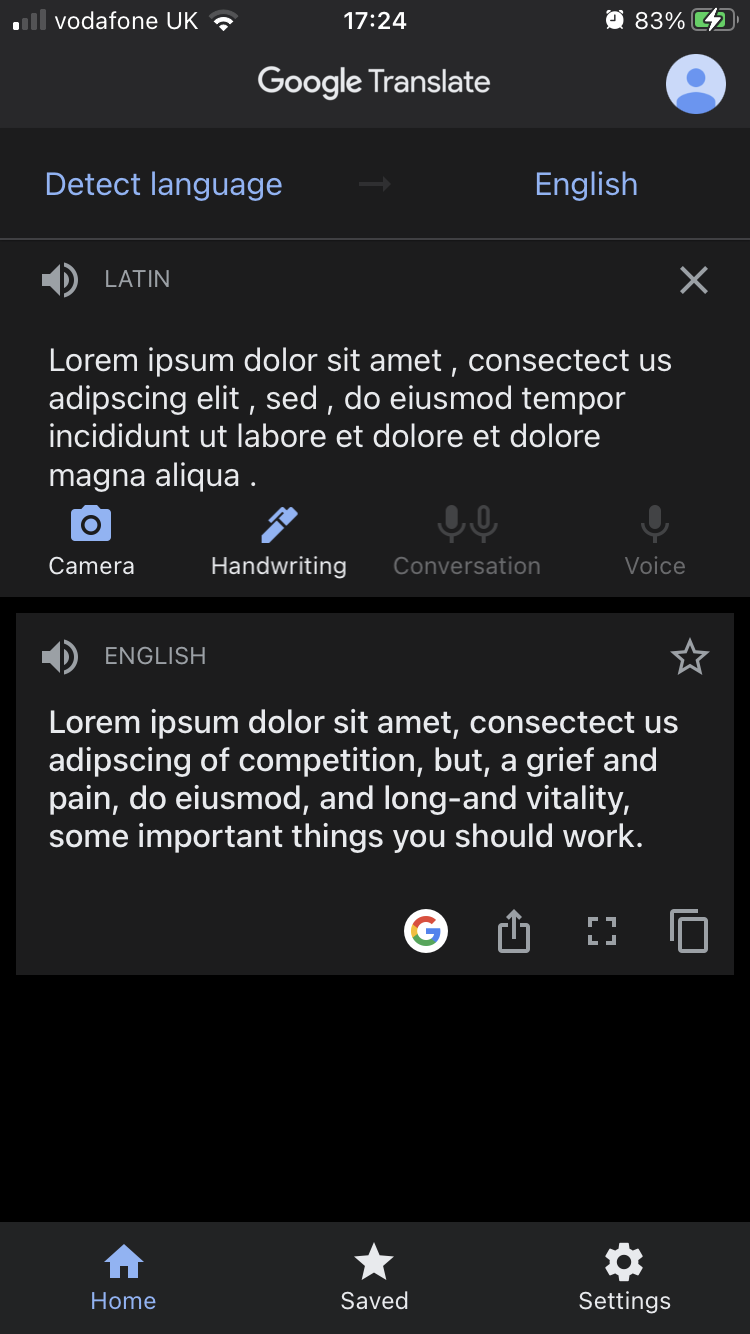
\includegraphics[width=2.1in]{Images/Google Translate/Main Tab.png}
\end{figure}
Above are screenshots of the main interface of the app. On the left is the input method and on the left is the output the app gives. 
\newline
Google Translate is a free smartphone app for Android or iPhone. The user takes a photo of a piece of text, which is passed through a pre-trained neural network, which translates it to a string. Then, the string is immediately translated to the target language. 
\newline
The app has a user-friendly interface that is simple to navigate and gives clear instructions at each stage. The layout is also easy to use as it uses a touch-screen display, making it intuitive for the user to use. The app also grants control to the user by allowing them to select the exact words they wish to translate.
\newline
However, the app does not allow the user to just convert a document into a text document, instead translating the text immediately upon viewing. Moreover, it is only available on mobile devices, making it useless for people like teachers, who will need the output given on a computer as this is the most common environment for working on documents or for writing. Furthermore, the app doesn't allow the user to train a personalised network, to make the program more accurate while translating. This would be useful when translating hard to read hand-writing.
\newline
\newline
\textbf{Applicable Features:}
\newline
I will try to emulate the lightweight design of this application, as well as the accessibility of it. Moreover, I think that the feature of being able to take photographic input is very useful as it provides an effective method of inputting data to translate. I will therefore add the ability enable the user to input a .png file saved on their computer to my solution, where it will attempt to convert that to a text document. This would provide more functionality to my solution. 

\subsubsection{Photomath App}
\begin{figure}[H]
\centering
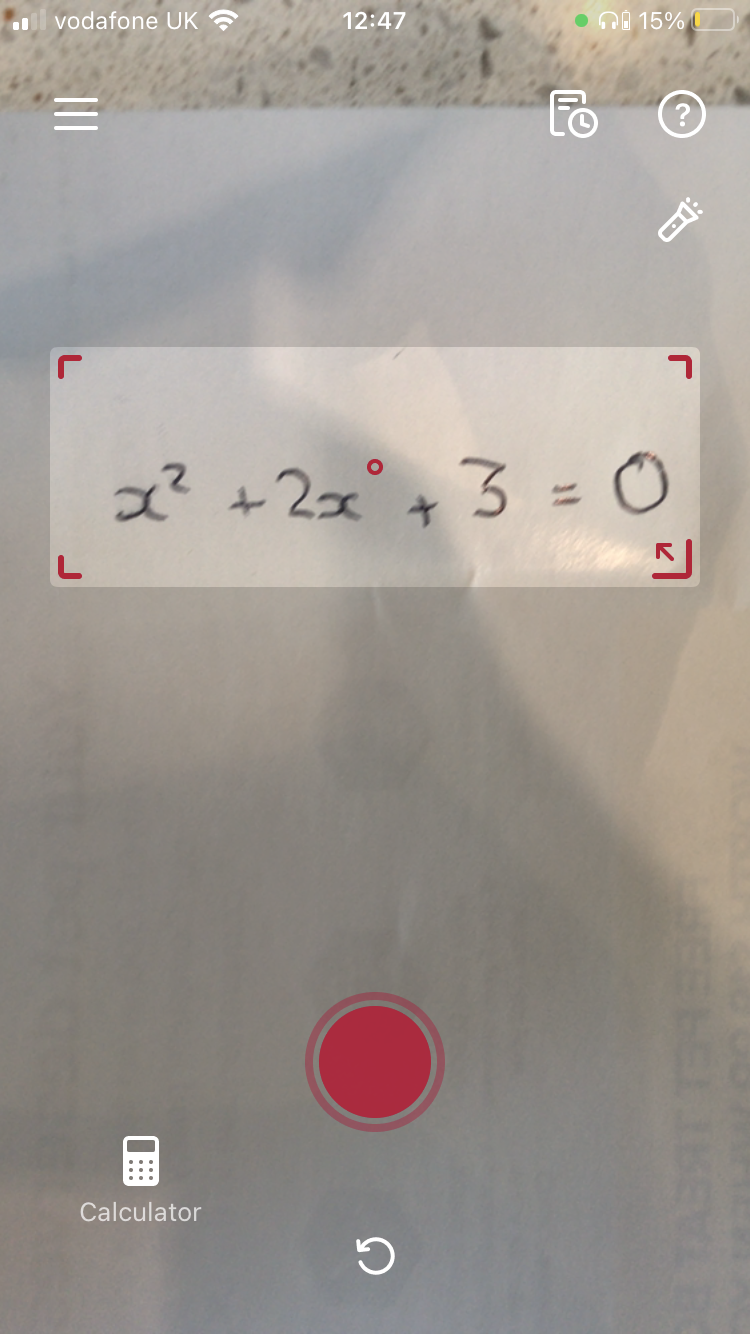
\includegraphics[width=2.1in]{Images/Photomath/Character Recognition.PNG}
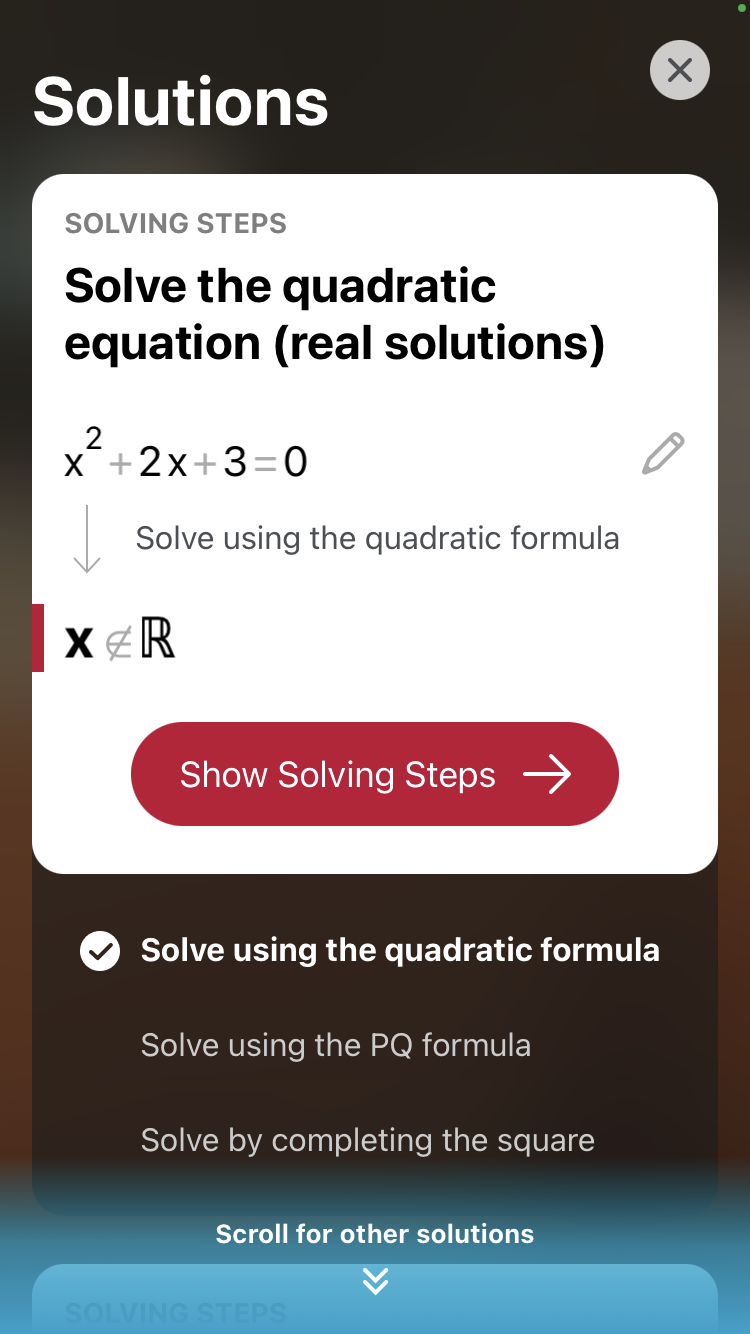
\includegraphics[width=2.1in]{Images/Photomath/Solution Tab.PNG}
\end{figure}
Above are the main parts of the user interface, the user takes a photo of an equation within the rectangle and then the program goes to the screen on the right which shows the equation and the solution.
\newline
Photomath is a free smartphone application available on Android and iPhone. It consists of a main page where users can take photographs of maths problems, which will then be translated to a string. After it has been translated, the program can then solve the problem and display its answer on the next page of the app. 
\newline
The app has a lightweight design, with few buttons and simplistic interface, which linearly takes the user through the stages of set-up. The camera page follows the normal design conventions of a camera, with the photo trigger being a circle in the bottom-centre of the screen. Another useful feature of it is that it can recognise handwriting as well as typed problems, which gives it more versatility and usefulness.
\newline
However, like the Google Translate App, it can't convert an image to an editable text document. This makes less useful for computerizing equations or maybe adding equations into a document by taking a photo of them. Another issue with this app is that it can only translate equations, as such it can't translate a written essay into a digital format. Moreover, it only works on a smartphone, and is not available for a computer user, limiting it for the same reason as the Google Translate App. Finally, a user can't translate a previously photographed equation. This is very limiting as the user has much less flexibility with the photos they want to translate, and cannot translate previously taken photos. This would be limiting to a teacher as they may not have direct access to the students work meaning they would not be able to use a photo a student has sent.
\newline
\newline
\textbf{Applicable Features:}
\newline
I will try to emulate the apps lightweight design, following normal design conventions to add familiarity for new users. This would make the program much easier to navigate for non-technical users. Since both this app and the Google Translate App don't allow the user to save the output text document to to the device, I will add in this feature to the program. Moreover, both apps don't allow the user to translate a previously taken photo. I will therefore add this functionality to the program as well.
\newpage
\subsection{Summary of Features}

\subsubsection{Initial Concept}
The solution will be program that can run on a computer. It will have a lightweight interface and be usable on start-up. It will do this by utilising accessible and intuitive design features like file pickers, buttons and check boxes. The user will be able to pick a image file from their computer to translate to text format using the interface. It will be accurate in its conversion of documents, making minimal mistakes and  will complete the conversion effectively. It will also output the resulting document to a file on the host machine, which will allow the user to immediately edit the document on their computer.
\newline
The program will work by reading the image and removing the noise in the image. The cleaned image will then be split up into its composite characters, these will then be sequentially passed through a neural network, which will translate the image to a character and add it to the output string. This resulting string will then be saved to a file on the user's computer.
\newline
The program will also have another tab, which will enable the user to train the neural network on a database of their own handwriting. This will improve the neural networks accuracy on their hand-writing, tailoring the solution to the user. To make the database creation simpler, the solution  will provide the user with instruction on how to set-up the database.

\subsubsection{Limitations}
The main limitation of my proposed solution is the compilation of the users database. Effective training data needs to be free of noise and there needs to be a lot of it. If I have time, a work-around will be allowing the user to just input a page of their handwriting and the program could use the image cleaning and splitting algorithms for the image translation to generate the database.
\newline
Another issue with this  solution is that it will take a relatively powerful machine to train a machine-learning model in a reasonable time-frame, due to the computational complexity of it. A solution would be to have a pre-trained model of the neural network packaged with the program, foregoing the necessity to train the neural network for each user. A user could then make use of the training feature to personalise the program on their specific hand-writing, but would not need to in order for the program to function.
\newpage

\subsection{Stakeholder Input}
I sent my stakeholders the following email to keep them updated on the progress:
\newline
\newline
Dear All,
\newline
I am sending you this email to update you on the progress of the program. I want your input on the current state of the project. 
\newline
It will have a lightweight design interface, using mainly buttons and file explorers to navigate the program. I will add in  the feature of provide the program with a data set of your own handwriting, to make it more personalised. There will two functions of the program, the aforementioned trainer and then the ability to input a photo from your computer and get the output on your computer. The only issue would be the training function would probably need a relatively powerful machine to make it run in a reasonable length of time.
\newline
\newline
Best Wishes,
\newline
Jacob Inwald
\newline
\newline
The responses I received are below:
\subsubsection{Isaac}
Sounds great! I really like the idea of being able to train on specific handwriting as mine is quite uniquely bad so that should increase accuracy. I have a powerful machine so the processing power shouldn't be an issue. Looking forward to seeing how it goes.
\subsubsection{Ethan}
I like the ability to input the photo of the document and get the corresponding file back to your computer. I don't have a very powerful machine, but that shouldn't be a problem because I probably won't use the personalisation feature a lot. 

\subsubsection{Michael}
Hi Jacob,
\newline
\newline
This sounds very good. I don't think I will use the personalisation feature a lot so the requirement for a powerful machine won't apply. As long as the interface is easy to use and I get a document back, it should be fine.
\newline
\newline
Kind Regards,
\newline
Mr Lawrence

\newpage

\section{Requirements}
\subsection{Hardware}
\textbf{A computer capable of running this program} - This program will use neural networks for the hand-writing recognition, meaning it will be computationally expensive to train the network on a user's handwriting. Although it will come prepackaged with a general neural network, a powerful processor will be required to do specific training on the user.
\newline
\newline
\textbf{Standard peripherals} - The program will also require the standard peripherals in order to operate it i.e. keyboard, mouse and monitor.
\subsection{Software}
\textbf{Windows, Mac or Linux operating system} - I will use Tkinter, Numpy, PIL and Python when coding this project, and they support these operating systems only.
\newline
\newline
\textbf{Numpy} - This is a library for python used for mathematical expressions which will be necessary for this program to work.
\newline
\newline
\textbf{Tkinter} - This is a library for python which is used to make graphical user interfaces (GUIs). I will use it in the creation of the user interface.
\newline
\newline
\textbf{PIL} - This is a library for python which is used to manipulate images and and image files. I will use this for he character tracing algorithms.
\newline
\newline
\textbf{Python} - All the code will be written in python so the target computer must have python installed with the base libraries as well.

\subsection{Stakeholder Requirements}

\subsubsection{Design}

\begin{table}[H]
\centering
\begin{tabular}{|l|l|}
\hline
\textbf{Requirement} &
  \textbf{Explanation} \\ \hline
Easy to navigate design &
  \begin{tabular}[c]{@{}l@{}}This will allow the user to make the most use of \\ the multi-functional program, enabling the user \\ to both train and run the network.\end{tabular} \\ \hline
Navigable file system &
  \begin{tabular}[c]{@{}l@{}}This will make it much easier for the user to save \\ the output of the program to a file on their system,\\ making it more accessible.\end{tabular} \\ \hline
Obvious way to shutdown program &
  \begin{tabular}[c]{@{}l@{}}Because the program may be resource intensive,\\ users could wish to shut down the program before \\ it is  finished running. This means a user can force \\ quit whenever they want.\end{tabular} \\ \hline
Simple interface &
  \begin{tabular}[c]{@{}l@{}}This will make sure users don't get confused by the\\ program and are able to use the program  \\immediately upon
  start-up.\end{tabular} \\ \hline
\end{tabular}
\end{table}


\subsubsection{Functionality}

\begin{table}[H]
\begin{tabular}{|l|l|}
\hline
\textbf{Requirement} &
  \textbf{Explanation} \\ \hline
Output to a file &
  \begin{tabular}[c]{@{}l@{}}This was a feature that a lot of the stakeholders\\ wanted; it would make it easier to manipulate the\\ file after translation.\end{tabular} \\ \hline
\begin{tabular}[c]{@{}l@{}}Ability to personalise the program\\ to the user\end{tabular} &
  \begin{tabular}[c]{@{}l@{}}This was mentioned by Isaac, and would be a \\ great addition to improve the usefulness of the \\ design. Having the option to make the program\\ more tailored to the user would be very useful.\end{tabular} \\ \hline
\begin{tabular}[c]{@{}l@{}}Is relatively quick to translate \\ documents\end{tabular} &
  \begin{tabular}[c]{@{}l@{}}This would be necessary to make the program \\ useful to people like teachers, who have large \\ quantities of work that would need to be \\ translated to a digital format.\end{tabular} \\ \hline
\begin{tabular}[c]{@{}l@{}}Is relatively accurate in its \\ translation\end{tabular} &
  \begin{tabular}[c]{@{}l@{}}Michael mentioned that the previous program he \\ had tried wasn't that accurate, which was why it\\ wasn't useful. This means that my solution needs\\ to be quite accurate in its translation.\end{tabular} \\ \hline
\end{tabular}
\end{table}


\subsubsection{Hardware}

\begin{table}[H]
\centering
\begin{tabular}{|l|l|l|l|}
\hline
\textbf{Component} &
  \textbf{Minimum} &
  \textbf{Recommended} &
  \textbf{Explanation} \\ \hline
Processor &
  \begin{tabular}[c]{@{}l@{}}x86 64 bit processor\\ 1GHz clock speed\end{tabular} &
  \begin{tabular}[c]{@{}l@{}}x86 64 bit processor\\ 3.2GHz clock speed\end{tabular} &
  \begin{tabular}[c]{@{}l@{}}While the base requirements\\ of python are quite low, I \\ would recommend a fast\\ processor for the training \\ part of my program.\end{tabular} \\ \hline
Peripherals &
  \begin{tabular}[c]{@{}l@{}}Mouse, Keyboard\\ and Monitor\end{tabular} &
  See Minimum &
  \begin{tabular}[c]{@{}l@{}}A mouse and keyboard will\\ be required to interact with\\ the program so those are\\ necessary. The monitor will\\ also be necessary for provide\\ output to the user.\end{tabular} \\ \hline
RAM &
  4GB &
  16GB &
  \begin{tabular}[c]{@{}l@{}}A lot of RAM is not necessary\\ for the function of the base \\ program, but for the training\\ part of the program, a lot of \\ RAM will be used so that is\\ needed\end{tabular} \\ \hline
\begin{tabular}[c]{@{}l@{}}Free Disk\\ Space\end{tabular} &
  8GB &
  See Minimum &
  \begin{tabular}[c]{@{}l@{}}8GB of free diskspace will\\ be needed to store the data\\ for training and to store \\ python on the computer. So\\ this is the minimum amount\\ of free disk space needed \\ for the program\end{tabular} \\ \hline
\end{tabular}
\end{table}

\newpage

\section{Success Criteria}

\begin{table}[H]
\centering
\begin{tabular}{|l|l|}
\hline
Success Criteria &
  Evidence \\ \hline
Working Tab System &
  \begin{tabular}[c]{@{}l@{}}Screenshots of the different tabs after switching\\ to them\end{tabular} \\ \hline
\begin{tabular}[c]{@{}l@{}}Main tab with the interface for translating\\ an image into a text file in it\end{tabular} &
  \begin{tabular}[c]{@{}l@{}}Screenshot of the main tab, with the intended\\ interface shown\end{tabular} \\ \hline
Simple and lightweight design &
  \begin{tabular}[c]{@{}l@{}}Screenshot of the two different tabs, showing a\\ simply laid-out and uncluttered interface\end{tabular} \\ \hline
\begin{tabular}[c]{@{}l@{}}Training tab with the interface for training\\ the network on an users desired database\end{tabular} &
  \begin{tabular}[c]{@{}l@{}}Screenshot of the training tab, with the \\ intended interface shown\end{tabular} \\ \hline
Ability to save output file to computer &
  \begin{tabular}[c]{@{}l@{}}Screenshot of text-file in output folder and a \\ screenshot of the code responsible for it\end{tabular} \\ \hline
\begin{tabular}[c]{@{}l@{}}Ability to train a new network on an users\\ desired database\end{tabular} &
  \begin{tabular}[c]{@{}l@{}}Screenshot of the new save file made from the\\ user's database and screenshot of code \\ responsible for it\end{tabular} \\ \hline
Ability to use user trained networks &
  \begin{tabular}[c]{@{}l@{}}Screenshot of the user's trained network being \\ selected for translation\end{tabular} \\ \hline
Ability for low-end computers to run it &
  \begin{tabular}[c]{@{}l@{}}Screenshot of CPU usage while program is \\ running\end{tabular} \\ \hline
\begin{tabular}[c]{@{}l@{}}Program can translate a written document\\ into a text file\end{tabular} &
  \begin{tabular}[c]{@{}l@{}}Screenshot of input file and screenshot of\\ output text file\end{tabular} \\ \hline
\begin{tabular}[c]{@{}l@{}}Option to press a button to stop the\\ program translating an image\end{tabular} &
  \begin{tabular}[c]{@{}l@{}}Screenshot of button and screenshot of the\\ code responsible for the button\end{tabular} \\ \hline
\begin{tabular}[c]{@{}l@{}}Option to press a button to stop the\\ program training on a user database\end{tabular} &
  \begin{tabular}[c]{@{}l@{}}Screenshot of button and screenshot of the\\ code responsible for the button\end{tabular} \\ \hline
\begin{tabular}[c]{@{}l@{}}Text on each interactable object without \\ typos\end{tabular} &
  \begin{tabular}[c]{@{}l@{}}Screenshot of both tabs, with all text on it \\ without typos\end{tabular} \\ \hline
\begin{tabular}[c]{@{}l@{}}Dialogue boxes pop-up to explain what\\ things do where required\end{tabular} &
  \begin{tabular}[c]{@{}l@{}}Screenshot of all the dialogue boxes included\\ in the program\end{tabular} \\ \hline
\begin{tabular}[c]{@{}l@{}}All the buttons in the program work as\\ intended\end{tabular} &
  \begin{tabular}[c]{@{}l@{}}A screenshot of the code, button and testing for\\ each button in the program's interface.\end{tabular} \\ \hline
\begin{tabular}[c]{@{}l@{}}The program completes translation in a\\ reasonable amount of time i.e. a\\few hours or less for a large image\end{tabular} &
  \begin{tabular}[c]{@{}l@{}}Screenshot of complex image and python shell\\log of time taken.\end{tabular} \\ \hline
\end{tabular}
\end{table}


\chapter{Design}

\section{Problem Breakdown}
\subsection{Overview}
The problem will consist of a few smaller problems, which can be broken down into simpler functions. These sections are:
\begin{enumerate}
    \item The neural network
    \item Some image formatting to turn user input into a valid input for the neural network
    \item The graphical user interface
\end{enumerate}
These 3 sections are the basic parts of the program necessary for the solution to function. We can then breakdown these larger sections into their composite problems and solve these ones individually. This will make coding these sections much easier to do. Thus, the steps that I will follow are below:
\begin{enumerate}
    \item Code the basic algorithms for the neural networks i.e. save to file or load from file.
    \item Code the more complex algorithms like the back propagation algorithm and test them thoroughly.
    \item Put these complex algorithms together to create a working neural network.
    \item Set up functionality to read input from images.
    \item Code an algorithm to extract a character from an image based on a start pixel.
    \item Expand this to work for multiple characters in an image.
    \item Add a graphical front-end to this recognition feature.
\end{enumerate}
These steps will be the best way to approach the problem as they split the problem down into a series of more achievable problems. This will make the process of creating the program much easier
\subsubsection{Step Breakdown}
In \textbf{step 1}, I will make a strong foundation for the program, fully testing each function to prevent issues arising in the future. These functions will include everything from mathematical functions to structural functions, like initialising the network with random values.
\newline
\newline
In \textbf{step 2} the more complex functions used for training the neural network will be coded by utilising the simpler functions programmed in \textbf{step 1}. This will enable me to focus on implementing these algorithms correctly, without having to worry about implementing the core functions necessary for those algorithms to work. Due to the complexity of some of these algorithms, I will be unable to use input-output testing to test them. Instead, I will look at the logic flow within the algorithm to find bugs. In \textbf{step 3} I will be able to fully test the program, which will enable me to find any bugs I missed before.
\newline
\newline
\textbf{Step 3} will consist of putting the functions written in \textbf{steps 1 and 2} together to create the functional neural network. The main purpose of this stage is to catch any bugs that the previous two stages missed. I will do this by using a performance metric for the network that will track how effectively the network trains. This will enable me to detect any abnormalities in the training process and then locate the source of those problems.
\newline
\newline
In \textbf{step 4} I will program the simpler image cleaning functions. These will include removing noise, loading images from paths, finding boundaries of images and centering images. These functions will normalise the input to a form that the network can read. The aim of this step is to make inputs given as close as possible to the neural networks training data to improve accuracy and also to provide a foundation to work off while creating the more complex algorithms.
\newline
\newline
\textbf{Step 5} will consist of developing an algorithm that will crop a shape from an image. This will enable the program to separate the different characters in an image so they can be translated individually. Due to the complexity of this algorithm, it is being tested separately from the rest of the other algorithms to ensure that it won't create any problems later on.
\newline
\newline
In \textbf{Step 6}, I will develop the character cropping algorithm further by expanding it to work on an image with multiple images. This step is required as it means that the character cropping will already be fully functional before implementing it in the program. This will allow me to narrow down the cause of bugs easier.
\newline
\newline
\textbf{Step 7} will be where I put the whole program together and create the user interface for the front end. This step will not take long to code as there are no more extremely complex algorithms to create.
\newline
\newline
This step-by-step method will result in a very robust program, with any possible problems being prevented before they can cause any issues. The steps also split the complex problems into smaller problems, utilising the design philosophy of 'Divide and Conquer'. Moreover, the method is conducive for iterative design as it will iteratively improve upon each step.
\newpage


\section{Structure Of Program}

\subsection{Overview}
The structure of this program will be vital to this project working. It needs to be simple and easy to expand.

\subsubsection{Custom Library}
Before programming the complex parts of this solution, I will create a custom library with all the necessary functions for the neural network. This library will also contain all the image manipulation functions, making it easier to expand upon later on in the project.

\subsubsection{Neural Network}
The neural network is at its core a fully connected graph of nodes. I will structure this by using a two-dimensional array of nodes, with each node storing their connections to the other nodes. These connections will then be represented by using two arrays of tuples, where the tuples have a pointer to a connected node and the associated weight. One array will be for the backward connections and the other will be for the forward connections. 
\newline
These connections are necessary for feeding information forward through the network to get an answer, and for looping back through the network to improve its answers. This structure will allow me to easily find or change the input and output connections for each node during in the training process.

\subsubsection{User Interface}
The user interface will just be a front-end to the rest of the project, so will simply be structured as a class with all the necessary user functions in it and then call the rest of the project.

\subsection{Flow of Information}
In this section, I will show the flow of information through the program using a few flowcharts. The key for the flowcharts is as follows:
\newline
\textbf{Red lines} - Places where information flows back to a previous location, normally due to a loop.
\newline
\textbf{Curved Boxes} - Places where user action can be taken.
\newline
\textbf{Sharp Boxes} - Places where actions are performed by the program.
\newline
\textbf{Grey Boxes} - Places where information flows out to a different part of the program.

\subsubsection{General Layout}
\begin{figure}[H]
    \centering
    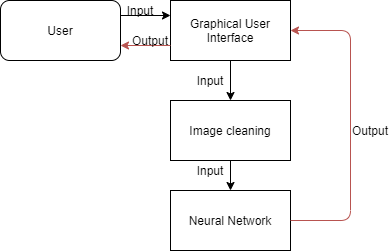
\includegraphics[width=12cm]{Images/Structure Of Program/Information Flow in Program Flow chart.png}
\end{figure}
This figure shows the flow of information through the different sections of the program. Information will flow from the user, through the interface to the image cleaning and then to the neural network and out to the user again. Since the user's input flows through the interface, I have more control over the inputs they give and can validate them accordingly.

\subsubsection{Neural Network}
\begin{figure}[H]
    \centering
    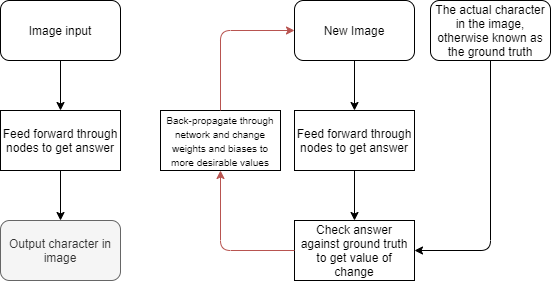
\includegraphics[width=12cm]{Images/Structure Of Program/Flow of infomation through neural network.png}
\end{figure}
Shown on the left is the flow of information when the neural network is identifying a character. I have ensured that no excess steps have been taken, which will make the process efficient and simple to program.
\newline
Shown on the right is the flow of information during the neural networks training loop. The two boxes at the top show the two inputs that  the network takes in to train, the ground truth and associated image. The neural network uses the image to create a prediction as to what it is and then compares that prediction against the ground truth. It will then use this comparison to improve its future predictions.

\subsubsection{Graphical User Interface - Main Tab}
\begin{figure}[H]
    \centering
    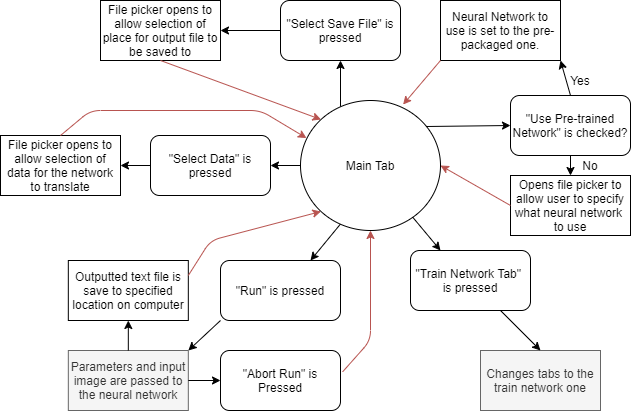
\includegraphics[width=13cm]{Images/Structure Of Program/Diagram for Main Tab.png}
\end{figure}
This figure shows the flow of information through the main tab. This will allow the user to select an image from their desktop to translate into a text file. The different options that the user can take are shown in the flowchart, with the results of these actions shown as the next step of the chain.

\subsubsection{Graphical User Interface - Training Tab}
\begin{figure}[H]
    \centering
    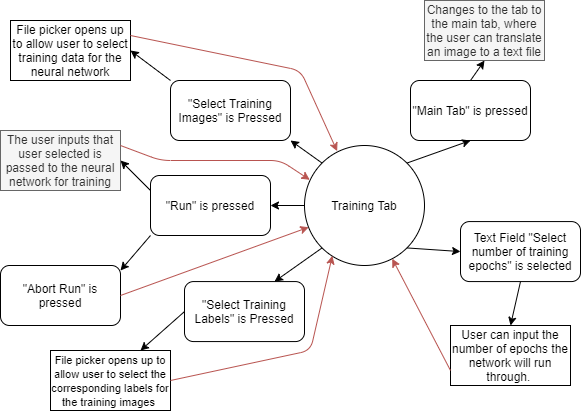
\includegraphics[width=12cm]{Images/Structure Of Program/Flowchart for Training Tab.png}
\end{figure}
This figure shows the flow of information through the training tab. This will allow the user to select the data necessary for the training process of the neural network. The different options that the user can take are shown in the flowchart, with the results of these actions shown as the next step of the chain.
\newpage

\section{Algorithms}
In this section, I will plan and explain the algorithms that will make up this project. These will range from the complex to the simple, and will cover the first two stages. I am not including the User Interface stage as it contains no algorithms that require planning

\subsection{Neural Network Algorithms}
\subsubsection{Part 1 - Basic Algorithms}
These are the simpler algorithms that will provide a base for the rest of the algorithms to build off of. They will include: generating a network with random weights and biases, saving to a file, loading from a file and a few more. These are all highly dependent on the way the network will be implemented, so the following pseudo-code is quite general and I will only plan out the first three algorithms mentioned.
\newline
\newline
\textbf{Initialising the neural network}
\newline
This function will initialise all of the nodes that form the neural network and then link them in layers with randomised weights and biases. The function will take in an array, which holds the number of nodes in each layers. For example, the array [2, 3, 4] would represent a network with two input nodes, three hidden nodes and four output nodes.
\newline
The method I will take to implementing this fully connected network in code is as follows. Each node will be represented by a node class, which will store the nodes in the layers on the left and right of that node in two arrays. These arrays will also hold the weights associated with each of these connections to the nodes in the other layer. Then a 2 dimensional array in the main network class will store all of the nodes in the network layers
\begin{verbatim}
PROCEDURE generateNetwork(nodeNumbers):
    network = [] # This is the variable that will hold all of the nodes
    for the network
    FOR i IN range(nodeNumbers.length):
        FOR x IN range(nodeNumbers[i]):
            network[i].append(a new node class with a random activation
            and bias)
    
    # set weights for input weights
    FOR i IN range(network.length):
        IF i == 0: # To skip the first layer, which has no input nodes
            continue
        loop through network[i] and set the input weights of each node 
        to random values
    
    # set weights for output weights
    FOR i IN range(network.length - 1): # We skip the last layer as it
    has no output nodes
        loop though network[i] and set the output weights of each node
        to the corresponding input weight
\end{verbatim}
\newpage
\noindent \textbf{Saving and Loading the neural network}
\newline
This function will save the current state of a network to a file on the computer. It will loop through the network and log the weights in the file using delimiters to separate the nodes and layers. It will then do the same for the biases, placing a delimiter in between the weights and biases.
\begin{verbatim}
PROCEDURE saveNetwork(network, filepath):
    string = ""
    FOR a IN range(network.length):
        add a "#" to the string
        FOR b IN range(network[a].length):
            add a "~" to the string
            FOR c IN range(network[a][b].inputNodes.length):
                add "," to the string
                add network[a][b].inputNodes[c] to the string
                
    add a "|" to the string
    
    FOR a IN range(network.length):
        add a "#" to the string
        FOR b IN range(network[a].length):
            add a "~" to the string
            add network[a][b].bias to the string
            
    save the string to a text file on the file path specified
\end{verbatim}
To load from the file, the algorithm will simply perform these steps in reverse, splitting up the file at every delimiter. This will produce a list of weights and biases, which can then be loaded into the network. As this code will be quite simple to program, there is no need to plan it out as well.

\newpage

\subsubsection{Part 2 - Complex Algorithms}

\textbf{Neural Network Theory}
\newline
Neural networks are essentially interconnected networks of nodes with weighted connections, which can emulate the way humans learn. This is done through using a heuristic called the back propagation algorithm.
\begin{figure}[H]
    \centering
    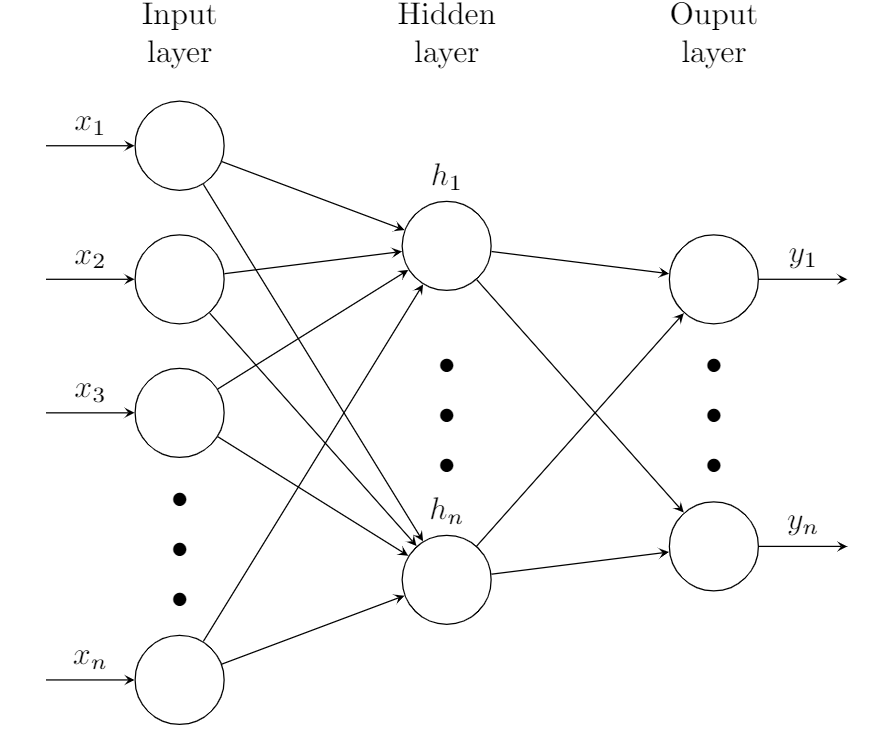
\includegraphics[width=10cm]{NeuralNetworkStructure.png}
    \label{fig:Network Structure}
\end{figure}
\noindent Shown above is the structure of the network. It consists of 3 layers of nodes: the input layer, hidden layers and output layer. Each node in each layer is connected with all the nodes in the layers on their left and right, with each connection between nodes being given a weight that represents the strength of that connection. Each node also has an activation, which represents how active the node is as a result of its input nodes; I will call this the nodes output. This activation is given by the sum of the activation of each input node multiplied by the strength of its connection to the current node. This means that the stronger a connection between two nodes, the more their activations will affect each other.
\newline
By assigning the input nodes with activations, the network can then feed these activations forward until the output nodes have an activation, which is the networks prediction. This predictions is just a guess at first, but by adjusting the strength of each nodes connection we can improve the accuracy of the networks predictions. This is how a neural network trains.
\newline
\newline
An important note to make is the method by which the network provides an answer. This will use one-hot representations, where a number is represented by the position of a 1 in an array of 0s. For example, a 1 in a range between 1 and 5 would be \pyth{[1, 0, 0, 0, 0]} in a one-hot representation. This is required because the activations of the nodes take values between 1 and 0, which means that any output of the network will be represented by a one-hot representation, where the position of the largest number in the array is the answer the neural network gives.
\newpage
\noindent\textbf{Feed Forward Function}
\newline
This function will feed the activations of the input nodes through the network. Each node in the network takes the weighted sum of its input nodes activations, adds its bias and then puts this through its activation function, in this case a sigmoid function. This value becomes the nodes new activation.
\newline
The best way to implement this is by putting a feed forward function in the node class, then calling this function for every node in the network in a feed forward function in the network class. Below is the pseudo-code for the feed forward function in the node.
\begin{verbatim}
PROCEDURE feedForward():
    total = 0
    FOR i IN range(inputNodes.length):
        total += inputNodes[i][0].output * inputNode[i][1]
    z = total + bias
    output = sigmoidFunction(z)
END PROCEDURE
\end{verbatim}
This uses the algorithm described above to calculate the output of the node based on the state of its input nodes and the related connections. The pseudo-code below for the corresponding neural network function.
\begin{verbatim}
PROCEDURE feedForward():
    FOR i IN range(nodes.length):
         IF i == 0 THEN
                skip to next iteration
            FOR x IN range(nodes[i].length):
                node[i][x].feedForward()
END PROCEDURE
\end{verbatim}

\noindent\textbf{The Cost Function}
\newline
This function will give a quantitative measure of how good a prediction is. It takes in the correct answer (\pyth{TrueValue}) and the networks prediction (\pyth{Prediction}), and finds the square of the difference between the two arrays values. \pyth{TrueValue} is essentially what the values of the output nodes activations should be (the one-hot representation of the character in the input image) and \pyth{Prediction} is the array of the activations of the output nodes.
\newline
This measure will be vital while training the network, as the network will use the measure to find how far off a prediction is, and then change its internal state accordingly.
\begin{verbatim}
PROCEDURE evaluateCost(TrueValue, Prediction):
    cost = 0
    FOR i IN range(Prediction.length):
        cost += (Prediction[i] - TrueValue[i]) ** 2
    return cost
END PROCEDURE
\end{verbatim}
\newpage

\noindent
\textbf{The Back Propagation Heuristic}
\newline
This function will quantify the amount by which each weight and bias needs to change in order for the network to improve its predictions. This amount is known as the error of a node, and it will then be used to alter the weights and biases of that node in the \pyth{updateWeights} algorithm.
\newline
The error of a node is calculated by differentiating the cost function with respect to that node's weight or bias, found using the chain rule. This gives the gradient of the cost function at that node. We can then step the nodes weights and bias in the opposite direction of the gradient to minimise the cost. This idea is shown on the graph below, where the black arrows show the direction the network needs to go in order to get to a minima of the graph. This shows that for a negative slope, the weight needs to increase to minimise cost and for a positive slope, the weight needs to decrease to minimise cost. The differential gives an equation by which to calculate the gradient for a certain nodes weights or bias and then the error is simply the negative of that gradient.
\begin{figure}[H]
    \centering
    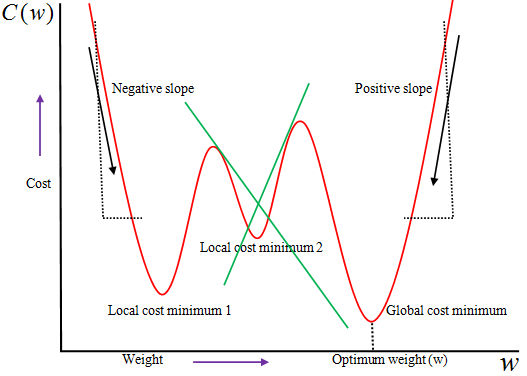
\includegraphics[width=4in]{Cost-Weight Explanatory Diagram.png}
    \label{fig:Cost-Weight Explanatory Diagram}
\end{figure}
\noindent On the next page the derivation of the equation used for the back propagation heuristic is presented.
\newpage

\noindent We can derive the equation used in this back propagation algorithm using differentiation and the chain rule like so:
\newline
\newline
Let the Cost Function be $C(x)$ where $C(x) = (x - x_{i})^2$ and $x_{i}$ is the intended value of $x$
\newline
\newline
Let the function to get $x$ (the final output of the node) be $x = \sigma(z)$, or the Sigmoid Function.
\newline
\newline
Let the function to calculate $z$ (The output before going through the sigmoid function) be $z = w_{p}x_{p} + b_{c}$. Where $x_{p}$ is the previous node's output and where $w_{p}$ is the weight connecting the previous node to the current node and $b_{c}$ is the bias of the current node.
\newline
\newline
Let the error of a node be $e$, given by $e = -\frac{d C(x)}{d x} $
So functions we have are:
\newline
$$C(x) = (x - x_{i})^2$$
$$x = \sigma(z)$$
$$z = w_{p}x_{p} + b_{c}$$
so if $$\frac{d C(x)}{d x} = 2(x - x_{i})$$
then $$\frac{d C(x)}{d z} = \frac{d C(x)}{d x} \times \frac{d x}{d z} = 2(x - x_{i}) \times \sigma^{\prime}(z)$$ 
thus $$e = -2(x - x_{i}) \times \sigma^{\prime}(z)$$
From the error we can find three things. The derivative of the cost function with respects to $w_{p}$ and $b_{c}$ and also the error of the previous node. This then repeats, propagating backwards until reaching the input layer, at which point, we know the error of all the nodes.
\newline
For the weight, its error (say $e_{w}$) is given by:
$$e_{w} = -\frac{d C(x)}{d w_{p}} = -\frac{d C(x)}{d z} \times \frac{d z}{d w_{p}} = e \times x_{p}$$
For the bias, its error (say $e_{b}$) is given by:
$$e_{b} = -\frac{d C(x)}{d b_{c}} = -\frac{d C(x)}{d z} \times \frac{d z}{d b_{c}} = e \times 1 = e$$
And for the previous nodes error ($e_{p}$) is given by:
$$e_{p} = -\frac{d C(x)}{d z_{p}} = -\frac{d C(x)}{d z} \times \frac{d z}{d x_{p}} \times \frac{d x_{p}}{d z_{p}} = e \times w_{p} \times \sigma^{\prime}(z_{p})$$
Where $z_{p}$ is the previous nodes z value.
\newline
So now that we know the equation for the error, all that remains is implementing it.
\newpage

\begin{verbatim}
PROCEDURE backPropagationHeuristic(trueValue):
        
    FOR node IN outputLayer:
        node.error = -2 * (node.output - trueValue) *
        sigmoidDerivative(node.z)
        
    FOR layer IN network:
        skip the first and last layer as we don't need 
        error for it and we already have the error for 
        the last layer.
        
        FOR node IN layer:
             cost = 0
            FOR record IN node.inputNodes:
                this inputNodes array will consist of                     
                the input nodes for the target node and
                the weights associated with them.
                    
                weight = record[1]
                inputNode = record[0]
                cost += inputNode.error * weight
            node.error = cost * sigmoidDerivative(node.z)
END PROCEDURE
\end{verbatim}

\noindent\textbf{Update Weights Algorithm}
\newline
This algorithm will use the error calculated in the back propagation heuristic to make the appropriate changes to the weights in the network. In essence it will increment each variable in the network by the error for that variable. To allow more control over the rate that the neural network learns at, this increment is multiplied by a float parameter named \pyth{learningPace}. The purpose of this parameter is to ensure the network won't stop improving its prediction too early.
\newline
The maths responsible for this is included in the proof above.
\begin{verbatim}
PROCEDURE updateWeights(self, learningPace):
    FOR layer IN network:
        skip the first layer as there is no need to find 
        error for it.
        
        FOR node IN layer:
            biasDelta = learningPace * node.error
            FOR record IN node.inputNodes:
                record[1] += biasDelta * record[0].output
                record[0].outputNodes[node.number][1] = record[1]

            node.bias += biasDelta
            node.error = 0
END PROCEDURE
\end{verbatim}
\newpage

\subsection{Computer Vision Algorithms}
\textbf{Clean Image Algorithm}
\newline
This function will remove noise from the image to enable the edge tracing algorithm to work. This works by compressing the pixels colours into the range of 0-1 and then removes any pixels that are below a threshold colour. This will ensure that there is no extraneous noise when cropping out the characters.
\begin{verbatim}
PROCEDURE cleanImage(image):
    array = []
    adjust = 0.99 / 255
    FOR y IN range(image.height):
        FOR x IN range(image.width):
            set white and black to the corresponding greyscale
            values, with 255 being the maximum value.
            IF ABS(white - black) * adjust > 0.1:
                array.append(ABS(white - black) * adjust)
            ELSE
                array.append(0)
    return array
END PROCEDURE
\end{verbatim}

\noindent \textbf{Edge Detection Algorithm}
\newline
This algorithm will trace the outline of a shape in an image, given a pixel in the image, then crop out the shape from the image and return the cropped out image.
\newline
This will work by moving from the starting pixel to adjacent coloured pixels, and adding each adjacent pixel to the new image. This will create an outline of the image, which can then be used to find the position that the algorithm should crop from to output the correct image.
\newline
However, the problem here lies in choosing the best pixel to jump to next. The solution that I will use is to hard code the correct set of priorities for the algorithm to use. These priorities can then be refined with rigorous testing of the algorithm during development.
\begin{verbatim}
PROCEDURE traceCharacter(startX, startY, img):
    characterFound = False
    numberPixels = []
    initialise tgtImg and cropImg as blank white images of
    the same dimensions as img.
    x = startX
    y = startY
    
    WHILE NOT characterFound:
        numberPixels.append([x, y])

        Put the pixel with the coordinate (x, y) 
        from img into tgtImg at the same position.
        
        Pick a new pixel with the coordinates (x, y) to jump to
        based on the priorities found by testing.
        
        If no new pixel with the coordinates (x, y) exist then
        exit the while loop.
    
    return tgtImg
END PROCEDURE
\end{verbatim}
\newpage

\section{Usability}
\subsection{Overview}
This program will have 2 tabs, each performing the different tasks of the program. This will split up the program into simpler chunks for the user, meaning that they don't get overloaded by information or choice. 
\newline
\newline
The \textbf{first tab} will be for the main function of the program, translating input images to text files. It will be structured to make it easy for the user to use immediately upon start-up. This will be by using different design archetypes that will enable familiarity for the user and create a lightweight and easy-to-use design for a complex program. I will also ensure that the forms of input are simple, to ensure a lack of confusion for the user.
\newline
\newline
The \textbf{second tab} will be for the secondary function of the program, allowing the user to train the network on a specified database of handwriting. Since the training process is complex to set-up, this user interface will have explanations of what to put in each field and how it affects the network. Additionally, it will abstract the more complex parameters to fill away from the user, preventing any user error.
\newline
\newline
Since I am giving a lot of input ability to the user, I will need to be very careful about the validation used. I will try to limit user choice at every stage, making sure that the choice they make are entirely closed and they are unable to do things that would cause the program to break.

\subsection{Translation Tab}

\begin{figure}[H]
    \centering
    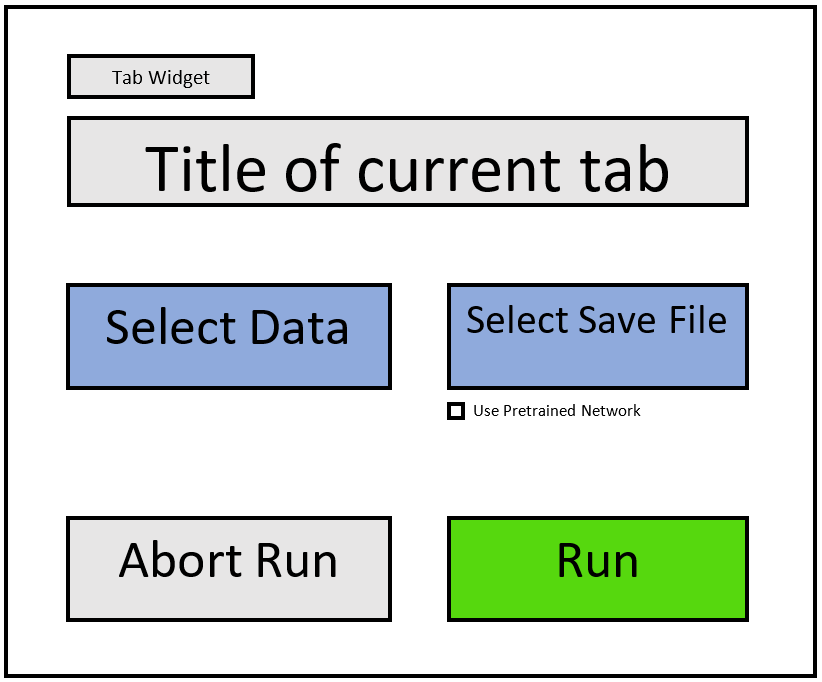
\includegraphics[width=12cm]{Images/Graphical User Interface/Translation Tab.png}
\end{figure}
\noindent This tab is what the user will interact with in order to translate an input image into a editable text file. As such, it needs to be quick and easy to use from start-up. I will use colours and layout to convey the proper usage without any need for the user to read a manual. This will be done by following design paradigms (i.e. run buttons are green) and by clearly labelling each button. Moreover, the small amount of buttons on the design will make it very easy to understand and use. The reasoning for each features are as follows

\subsubsection{Tab Widget}
This is used to change what tab the user is in. As such it will follow the normal design standard for tab widgets; being placed in the top left corner of the window, which will improve familiarity for new users. Additionally, each of the tabs will be clearly labelled to tell the user what tab it redirects to, which will enable simple and easy usage of the tab system and will prevent any problems.

\subsubsection{Title of Current Tab}
The purpose of this is to display the current tab the user is using. This will prevent confusion when navigating the tab system, making sure the user knows what tab they are on at all points during navigation. It will use a large font and be placed at the top of the tab to maximise its effect by drawing attention to it.

\subsubsection{Select Data}
This button will open a file picker entitled "Select Image to Convert", which will allow a user to pick a file of their choice to translate. As such, the button will be very large and clearly labelled, making it easy to see and use. Additionally, the button will be blue to make it clearly distinguishable from its surroundings. Finally it is positioned in the centre of the window, representing the order of interactions within the screen.

\subsubsection{Select Save File}
This button will open a file picker entitled "Select Save File of Previous Network", which will allow a user to pick a previous save file of the neural network which the program will use to translate the image. As such, the button will be large and clearly labelled, making it easy to see and use. Additionally, the button will be blue to make it clearly distinguishable from its surroundings. Finally, if the "Use Pretrained Network" check box is checked, the button will appear greyed out. This will prevent any confusion with the usage of the interface.

\subsubsection{Use Pretrained Network Checkbox}
This determines whether or not the program will use a pre-packaged neural network for translation or a user trained one. This checkbox will start off checked, which shows the intended way to use the program. Upon unchecking the box, the select save file button will become active and will change colour,. This will prevent confusion about the usage of the save-file system for the user. Additionally, upon checking the box the "Select Save File" button will grey out, preventing the user from making a mistake when setting up the program.

\subsubsection{Abort Run}
This button aborts a run that's in the process of happening. This gives the user an option to prevent the program from using up all of the computers resources while it runs. Additionally, this button is positioned to the left of the run button and clearly labelled to make it clear to the user what it does. Finally, it will be greyed out before the run starts, to prevent any confusion for the user to the usage of it. Once the user can use it, it will change colour to red, following the normal design paradigms for stop buttons.

\subsubsection{Run}

This button starts a fresh run for the program. It will be positioned on the bottom right and be coloured green to make it easy for the user to understand what it does. This is because this follows the normal design paradigms for start buttons. Moreover, once the button is pressed, it will become greyed out to prevent any confusion as to whether it should be pressed again or not. 
\newpage


\subsection{Train and Test Tab}

\begin{figure}[H]
    \centering
    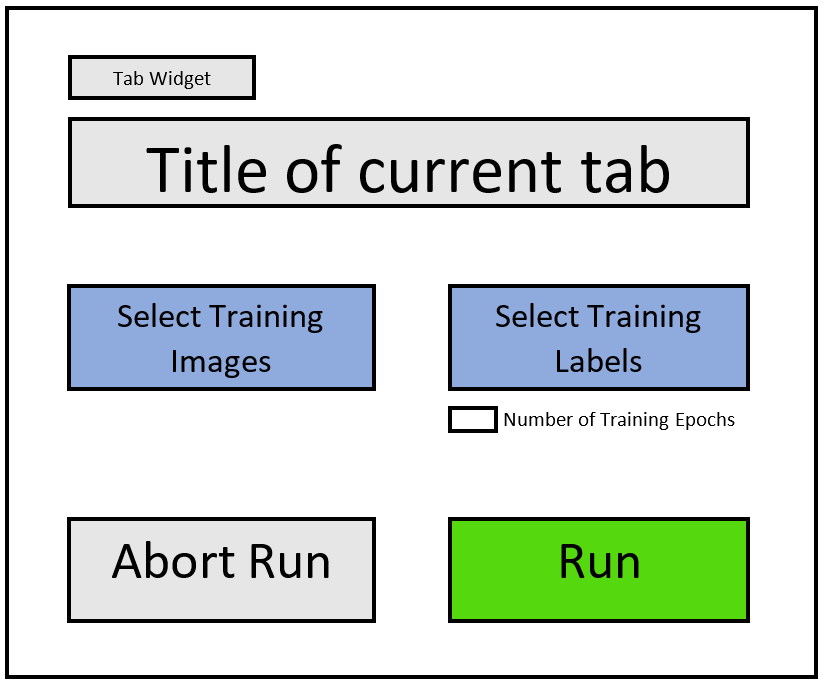
\includegraphics[width=12cm]{Images/Graphical User Interface/Training Tab.png}
\end{figure}

This tab is what the user will train the network on a user specified database. The interface will need to make a complex task simple. This will done by laying out the interface simply to make it easy to understand and use. To help achieve this, I will layout of the tab the same as the previous tab. This will aid familiarity with the program for the user as they have used it before. Moreover, the colours used on the different buttons will be the same, again improving the familiarity the user will have. Finally, the different methods of inputs will all be buttons, file-pickers or number fields. This will make it easy for the user to manipulate the interface, which each input requiring very simple actions to fulfill. The only difference between this tab and the previous one is be the substitution of the checkbox with a number field.

\subsubsection{Number of Training Epochs}
This field enables the user to enter a chosen number of training epochs for the neural network. This will give the user more control over the quality of training that the neural network will have. For example, the user can prevent the neural network over fitting on their data by reducing the number of epochs. This number field will be a drop-down menu so the user can select the number of epochs from this menu. This prevents the user from entering large numbers which will lead to a extremely long run time for large databases.
\newpage

\subsection{Validation}
In order for the program to be secure, it must have some forms of validation. This prevents bugs caused by bad user inputs. The data types the user can input and respective methods for inputting them are as follows:

\subsubsection{Buttons}
This input will be fine to validate, this is because they are entirely binary, meaning the user can only give one of two values as inputs. This removes all freedom from the user and prevents any error just because of this. Moreover, I will be using the in-built Tkinter buttons. These are already secure, and can make sure that an invalid input is not possible.

\subsubsection{Entering Path Files}
This input is a bit harder to validate, as allowing any file type could potentially be dangerous. To solve this I will make use of the in-built file explorer included in the Tkinter library. This allows me to avoid the problem of invalid inputs, while protecting against the possibility of dangerous file inputs. This is because using this system, I can protect against the user from select any other files other than the file type I want. Finally, in the case of save files or similar, I can validate them by putting a disguised key inside the save files to prevent the user from inputting random text files.

\subsubsection{Number Field}
This input is theoretically quite difficult to validate. This is because normally numbers are taken from text fields, which gives the user more freedom to pick numbers. However, in this case I want to restrict the number of epochs to whole numbers and restrict the magnitude of the number inputted. To avoid these errors, I will the input type will be a drop-down field with numbers up to 50 in it. This will prevent the user from entering any numbers too big for the program or in the wrong format for the program. This will again prevent incorrect user input.
\newpage

\section{Data Dictionary}

\subsection{Neural Network Variables}
These are the main variables that the program will use for the neural network:

\begin{table}[H]
\centering
\begin{tabular}{|l|l|l|ll}
\cline{1-3}
{\textbf{Name}} &
  {\textbf{Data Type}} &
  {\textbf{How it is used}} &
   &
   \\ \cline{1-3}
Network &
  \begin{tabular}[c]{@{}l@{}}A large 2D array that will store the\\ neuron data.\end{tabular} &
  \begin{tabular}[c]{@{}l@{}}To store the nodes in the network that the\\ neural network is composed of. It is \\ generated when the network is initialised.\\ It is then used in all the neural network\\ methods.\end{tabular} &
   &
   \\ \cline{1-3}
\begin{tabular}[c]{@{}l@{}}InputNodes \\ and \\ OutputNodes\end{tabular} &
  \begin{tabular}[c]{@{}l@{}}These are 2D arrays in the node\\ class that store the nodes' weights\\ and connections.\end{tabular} &
  \begin{tabular}[c]{@{}l@{}}This is used in the neural network methods\\ to keep track of the changes to the weights\\ and perform the calculations in the different\\ methods.\end{tabular} &
   &
   \\ \cline{1-3}
Z &
  \begin{tabular}[c]{@{}l@{}}This is a variable in the node class\\ that stores the z value of the node.\end{tabular} &
  \begin{tabular}[c]{@{}l@{}}The value is used in the back-propagation \\ algorithm. It is the weighted sum of all the\\ node outputs in the previous layer.\end{tabular} &
   &
   \\ \cline{1-3}
Output &
  \begin{tabular}[c]{@{}l@{}}This is also a variable in the node\\ class that stores the output of each\\ node.\end{tabular} &
  \begin{tabular}[c]{@{}l@{}}This value is used in the back-propagation\\ algorithm. It is the value of the Z after being\\ passed through the sigmoid function.\end{tabular} &
   &
   \\ \cline{1-3}
Number &
  \begin{tabular}[c]{@{}l@{}}This is a variable in the node class\\ that represents the nodes position \\ in its respective layer.\end{tabular} &
  \begin{tabular}[c]{@{}l@{}}This value is set when the neural network is\\ generated. It is used in other methods as an\\ identifier for the methods in the network.\end{tabular} &
   &
   \\ \cline{1-3}
Error &
  \begin{tabular}[c]{@{}l@{}}This is a variable in the node class\\ that stores the output from the \\ back-propagation method for that\\ specific node.\end{tabular} &
  \begin{tabular}[c]{@{}l@{}}This value is recalculated in every repetition\\ of the back-propagation heuristic. It is used\\ in the update weights class as well.\end{tabular} &
   &
   \\ \cline{1-3}
Path &
  \begin{tabular}[c]{@{}l@{}}This is a variable from the neural \\ network class. It stores the path \\ that the weights will be saved in.\end{tabular} &
  \begin{tabular}[c]{@{}l@{}}This is set when the neural network is \\ created, it specifies where the trained biases\\ and weights will be stored.\end{tabular} &
   &
   \\ \cline{1-3}
\end{tabular}
\end{table}

\newpage

\subsection{Character Tracing Variables}
These are the main variables that the program use in the character tracing program:

\begin{table}[H]
\centering
\begin{tabular}{|l|l|l|}
\hline
\textbf{Name} &
  \textbf{Data Type} &
  \textbf{How it is used} \\ \hline
Image &
  PIL image &
  \begin{tabular}[c]{@{}l@{}}It is the variable that stores the image\\ that the methods will work on.\end{tabular} \\ \hline
CharacterPixels &
  \begin{tabular}[c]{@{}l@{}}Array of tuples, each representing a\\ x, y position of a pixel.\end{tabular} &
  \begin{tabular}[c]{@{}l@{}}This variable is used in the character tracing\\ algorithm. It keeps track of which pixels are\\ part of the character.\end{tabular} \\ \hline
CharacterFound &
  Boolean &
  \begin{tabular}[c]{@{}l@{}}This variable is also used in the character \\ tracing algorithm. It tells the program \\ whether the entire character has been traced.\end{tabular} \\ \hline
OutputCharacters &
  Array of PIL images. &
  \begin{tabular}[c]{@{}l@{}}This variable is used in the character tracing\\ algorithm to keep track of the characters that\\ have been traced so far.\end{tabular} \\ \hline
\end{tabular}
\end{table}
\pagebreak

\section{Testing}

This section will demonstrate the method of testing the program that I will use. Each stage will require a different approach to testing due to the differences in the structure of them.
\newline
In general, my testing method will be quite simple:
\begin{enumerate}
    \item Test each function as I create it, catching simple errors
    \item Test the part of the program as a whole once I put all the functions together
    \item Check the complete program once completed by going through the intended steps.
\end{enumerate}
This follows an iterative development methodology, breaking the bigger problems into smaller easier to test issues. At each step of development, I will test the program as a whole, gradually creating a solid and bug-free program through iterative testing.
\newline
To help visualise some tests, I will use a library called \pyth{matplotlib} to chart different things during in the testing process. This will enable me to visualise how effectively the network is training or to display images. This will be extremely effective for functions like the training network one or the trace character one, where it is difficult to check that answers are correct based solely on numerical output.

\subsection{Neural Network Testing Method}

This part will be very difficult to test due to its complexity. I won't be able to fully check whether the program functions as intended until the neural network is put together, as most of the functions require each other to work. As such, I will rely mainly on run-time testing for \textbf{step 1} and \textbf{step 2} of development. I will catch errors in the functions during the creation of them, using test-data to check whether the function runs correctly. However, errors will inevitably slip through due to the reliance of some functions on others. Due to this, most of the important testing will occur in \textbf{step 3}. Due to the enormous amount of run-time variables and calculations occurring during the run of the program, I will have to rely mainly on black box testing for \textbf{step 3}. I will use test-data to train the neural network and then use the cost (see \textbf{section 2.3.1}) to see if it is getting more accurate throughout the training process. Depending on the pattern of cost I will be able to pinpoint an error. For example, if the cost is increasing there is probably a minus instead of a plus somewhere. Due to the iterative nature of this testing process, I will go from \textbf{step 3} to \textbf{step 2} multiple times as the testing at \textbf{step 3} will catch errors with code written in \textbf{step 2}. The iterative nature of this will help ensure that the code written from \textbf{step 1 - 3} is solid and secure.
\newline
For \textbf{step 3} I will use the MNIST online database. This is an open-source computer vision database specifically for training networks on optical character recognition. It has 60,000 images in it, split into a training database and a testing database. In order to iron out the bugs in the network, I will train and test the neural network using this database. This will give me a good metric of the accuracy of the neural network, and may find more bugs with the program that the first database wouldn't find.

\subsection{Character Tracing Testing Method}
The completion of this part of the program is dependent on a good testing method. This is because the character tracing algorithm relies on the correct set of priorities when tracing the image (see \textbf{section 2.3.2}). The only way to discover these priorities is by thinking of a good set and then testing its effectiveness. To do this, I will use test images as input and then check the quality of the output. This will be an iterative process, and won't take an extreme amount of time because the results of each test can be used to improve the code effectively.
\newline
The rest of the section can be tested similar to \textbf{steps 1 - 2} in the neural network, while writing the code. This will work well as each function is independent of the others, meaning that any issues are already narrowed down to their source.
\newline
For this section, I will use test data in the form of images, as that is what the functions will take as input. The source of these images will be the MNIST database. An example of these images is below:
\begin{figure}[H]
    \centering
    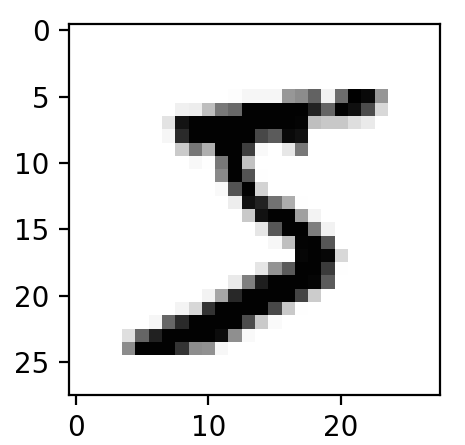
\includegraphics[width=5cm]{Images/Development and Testing/Method/Example MNIST Image.png} 
    \label{fig:MNIST input}
\end{figure}
\noindent The only issue with this test data is that it contains no noise, which is not representative of actual input the program will take. As such, I will have to also test the program's capability to handle real-world data. For this, I will use pictures of my handwriting to test the ability for the program to clean the image and crop out the characters within the image. This will give me the capacity to test how the program performs in real-life scenarios. An example of this test input is below:
\begin{figure}[H]
    \centering
    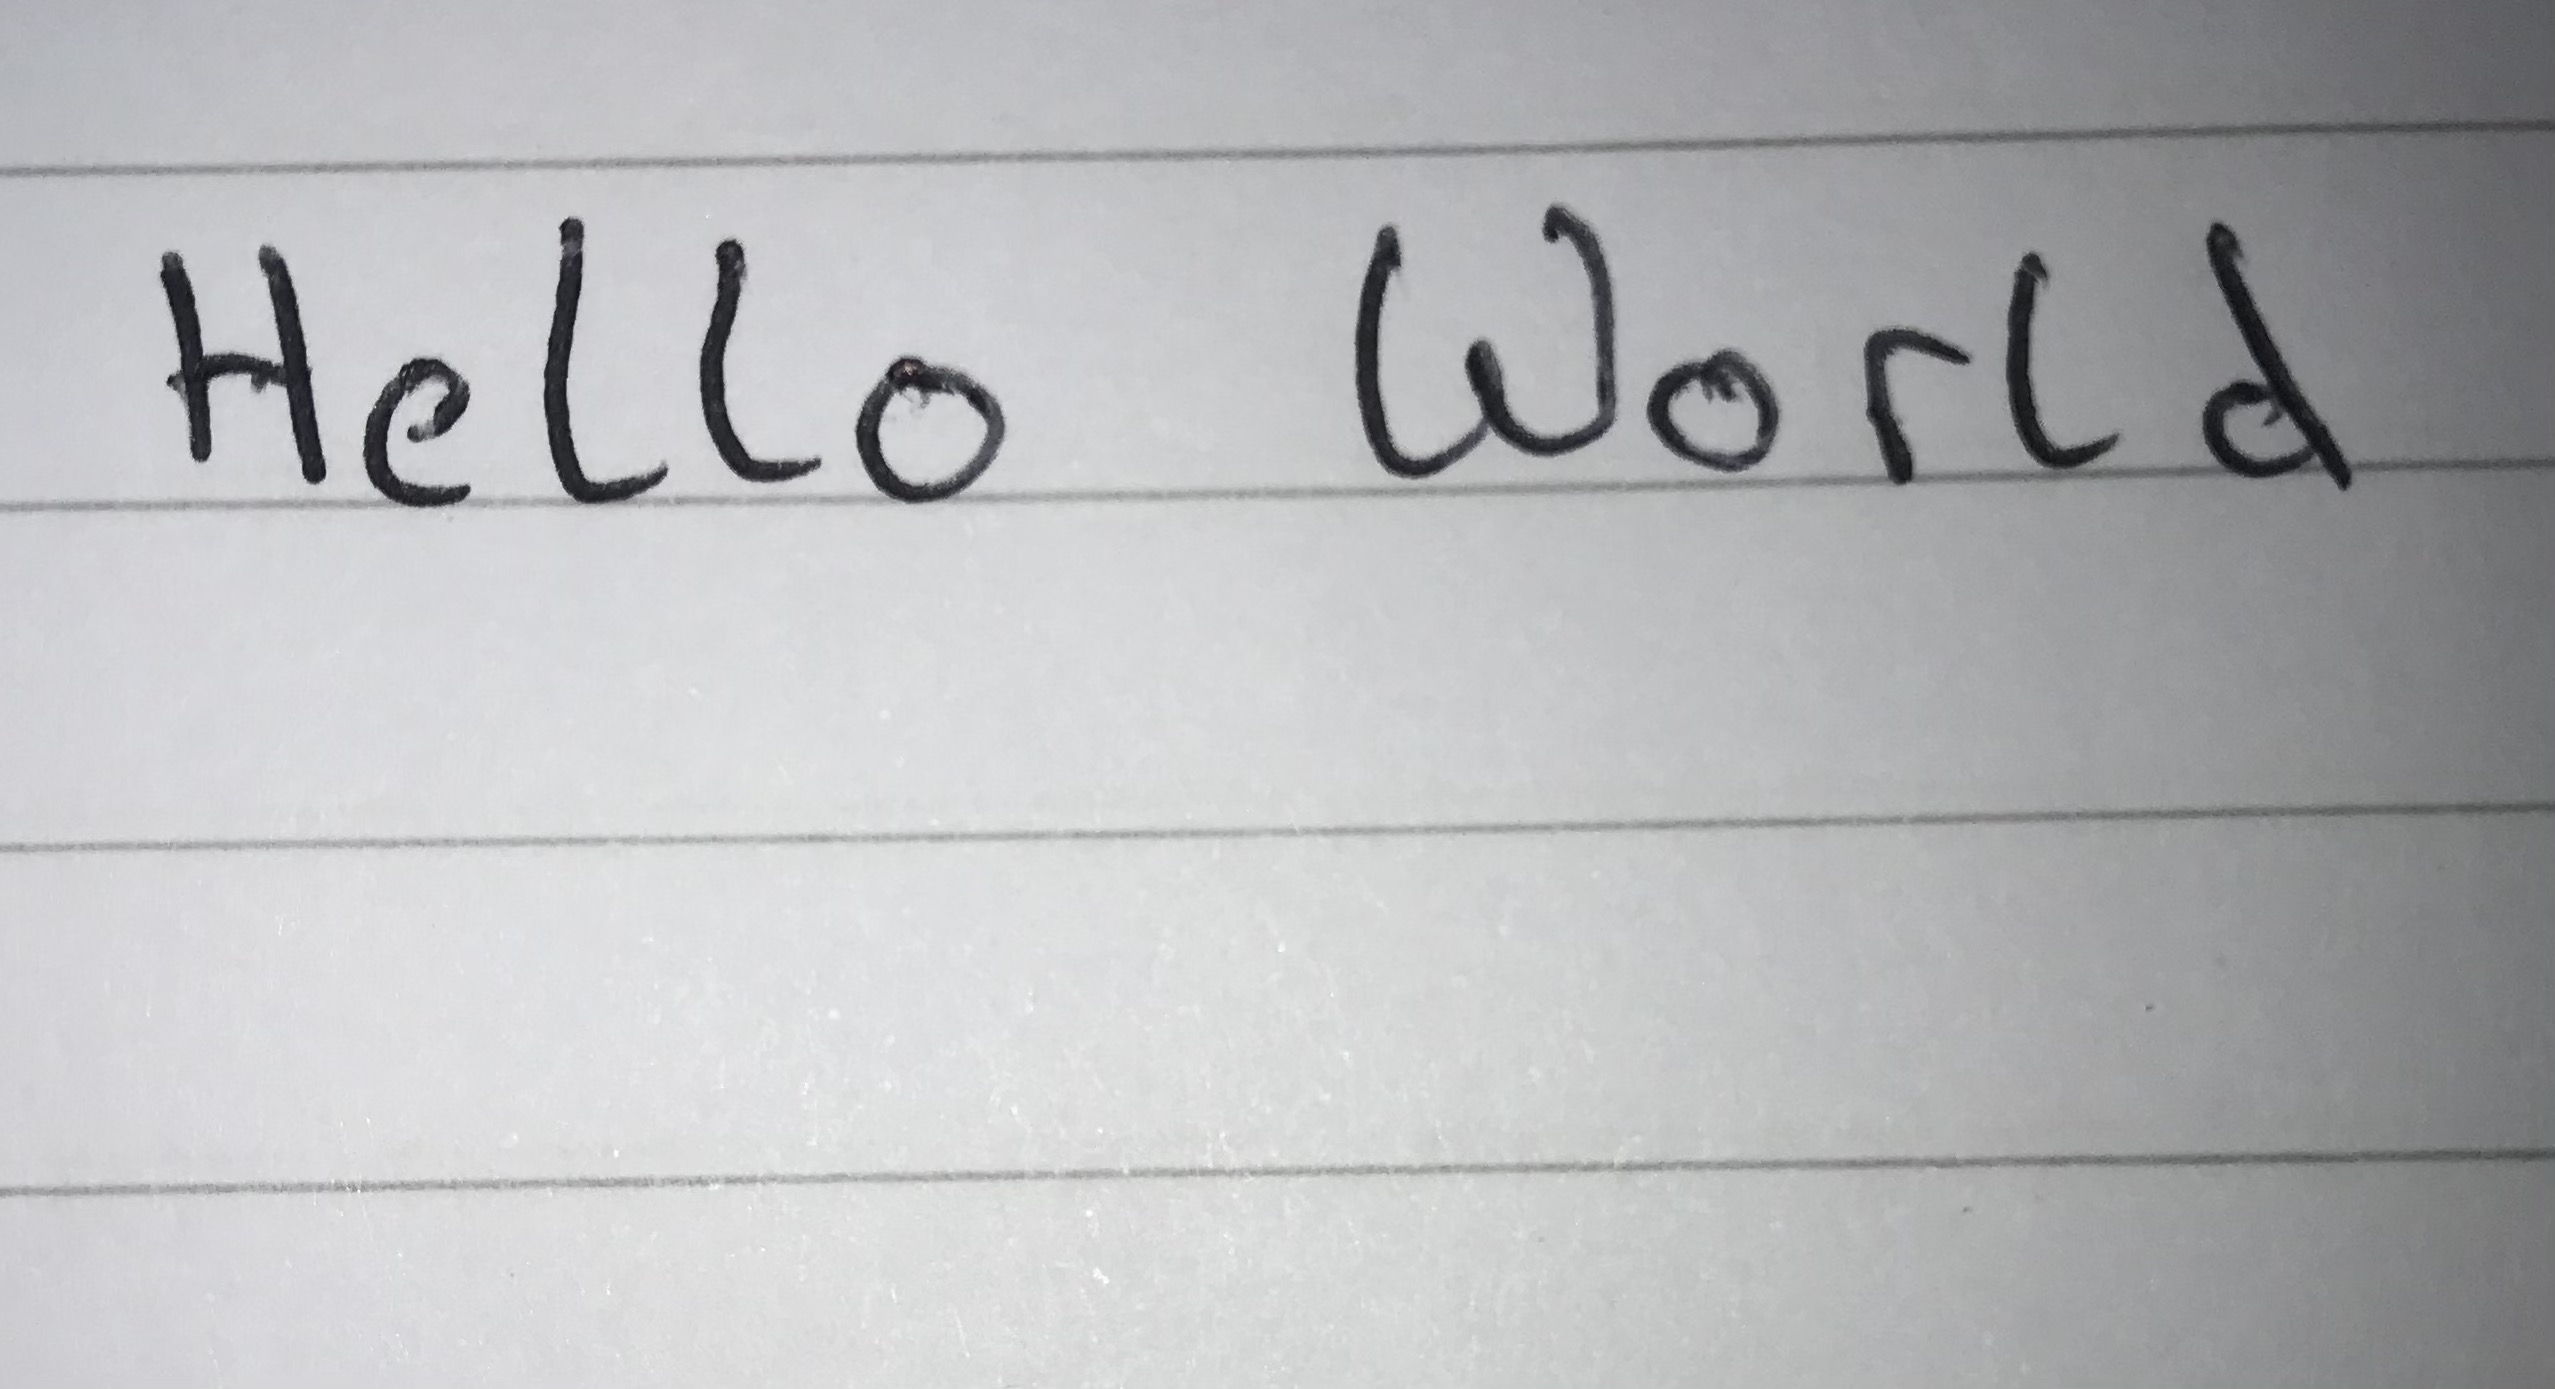
\includegraphics[width=5cm]{Images/Development and Testing/Method/Real-World Example.jpg} 
    \label{fig:Real World input}
\end{figure}
\noindent This image is a lot more complex and realistic to the input that the program will receive. It has shadows and The words are written on lined paper. These kind of images will be the final testing input for program functionality.
\newpage
\subsection{Graphical User Interface Testing Method}
This section will be where the majority of the destructive testing will occur. This is because the GUI is the first layer of interface with the user, so most the validation for the program will occur here. Moreover, this stage needs to look as intended, so the rest of testing will be checking correct formatting and functionality of the program. I will use a checklist to make sure everything is accounted for. There is a separate one for each tab.

\subsubsection{Translation Tab Checklist}

\begin{table}[H]
\centering
\begin{tabular}{|l|l|}
\hline
\rowcolor[HTML]{DAE8FC} 
\textbf{Test to perform}                                                                                                             & \textbf{Working?}        \\ \hline
\rowcolor[HTML]{CBCEFB} 
Check text for typos                                                                                                                 & \cellcolor[HTML]{CBCEFB} \\ \hline
\rowcolor[HTML]{DAE8FC} 
Check that Tab Widget works and changes the tab to what the user selected                                                            &                          \\ \hline
\rowcolor[HTML]{CBCEFB} 
Check that "Select Data" button opens a file picker when pressed                                                                     & \cellcolor[HTML]{CBCEFB} \\ \hline
\rowcolor[HTML]{DAE8FC} 
\begin{tabular}[c]{@{}l@{}}Check that the "Select Data" file picker prevents users from picking unwanted file\\ types\end{tabular}   & \cellcolor[HTML]{DAE8FC} \\ \hline
\rowcolor[HTML]{CBCEFB} 
Check that the "Select Data" file picker actually sets the data to the selected file                                                 & \cellcolor[HTML]{CBCEFB} \\ \hline
\rowcolor[HTML]{DAE8FC} 
Check that the "Use Pretrained Network" checkbox starts off pre-checked                                                              & \cellcolor[HTML]{DAE8FC} \\ \hline
\rowcolor[HTML]{CBCEFB} 
\begin{tabular}[c]{@{}l@{}}Check that a dialogue box pops up explaining to the user what will happen when \\ the checkbox is unchecked\end{tabular} &
  \cellcolor[HTML]{CBCEFB} \\ \hline
\rowcolor[HTML]{DAE8FC} 
\begin{tabular}[c]{@{}l@{}}Check that the "Select Save File" button is greyed out when "Use Pretrained\\ Network" is checked\end{tabular} &
  \cellcolor[HTML]{DAE8FC} \\ \hline
\rowcolor[HTML]{CBCEFB} 
\begin{tabular}[c]{@{}l@{}}Check that the "Select Save File" button cannot be pressed when "Use Pretrained\\ Network" is checked\end{tabular} &
  \cellcolor[HTML]{CBCEFB} \\ \hline
\rowcolor[HTML]{DAE8FC} 
Check that "Select Save File" button opens a file picker when pressed                                                                & \cellcolor[HTML]{DAE8FC} \\ \hline
\rowcolor[HTML]{CBCEFB} 
\begin{tabular}[c]{@{}l@{}}Check that the "Select Save File" file picker prevents users from picking\\ unwanted file types\end{tabular} &
  \cellcolor[HTML]{CBCEFB} \\ \hline
\rowcolor[HTML]{DAE8FC} 
\begin{tabular}[c]{@{}l@{}}Check that the "Select Save File" file picker actually sets the data to the selected \\ file\end{tabular} & \cellcolor[HTML]{DAE8FC} \\ \hline
\rowcolor[HTML]{CBCEFB} 
\begin{tabular}[c]{@{}l@{}}Check that the "Abort Run" button is greyed out and can't be pressed until the \\ "Run" button is pressed\end{tabular} &
  \cellcolor[HTML]{CBCEFB} \\ \hline
\rowcolor[HTML]{DAE8FC} 
\begin{tabular}[c]{@{}l@{}}Check that the "Abort Run" button becomes red and clickable after the "Run" \\ button is pressed\end{tabular} &
  \cellcolor[HTML]{DAE8FC} \\ \hline
\rowcolor[HTML]{CBCEFB} 
\begin{tabular}[c]{@{}l@{}}Check that the "Abort Run" button stops the program from running after being \\ pressed\end{tabular}      & \cellcolor[HTML]{CBCEFB} \\ \hline
\rowcolor[HTML]{DAE8FC} 
\begin{tabular}[c]{@{}l@{}}Check that the "Run" button is coloured green and becomes grey and \\ unclickable when it is pressed\end{tabular} &
  \cellcolor[HTML]{DAE8FC} \\ \hline
\rowcolor[HTML]{CBCEFB} 
\begin{tabular}[c]{@{}l@{}}Check that the "Run" button turns green and becomes clickable when "Abort \\ Run" is pressed\end{tabular} & \cellcolor[HTML]{CBCEFB} \\ \hline
\rowcolor[HTML]{DAE8FC} 
\begin{tabular}[c]{@{}l@{}}Check that the "Run" button starts the program running with the user's data\\  as input\end{tabular}      & \cellcolor[HTML]{DAE8FC} \\ \hline
\rowcolor[HTML]{CBCEFB} 
\begin{tabular}[c]{@{}l@{}}Check that the program saves the output file to the working directory of the\\ program\end{tabular}       & \cellcolor[HTML]{CBCEFB} \\ \hline
\end{tabular}
\end{table}

\newpage

\subsubsection{Training Tab Checklist}

\begin{table}[H]
\begin{tabular}{|l|l|}
\hline
\rowcolor[HTML]{DAE8FC} 
\textbf{Test to Perform}                                                                                                                      & \textbf{Pass?} \\ \hline
\rowcolor[HTML]{CBCEFB} 
Check text for typos                                                                                                                          &                \\ \hline
\rowcolor[HTML]{DAE8FC} 
Check that the Tab Widget works and changes the tab to what the user selected                                                                 &                \\ \hline
\rowcolor[HTML]{CBCEFB} 
Check that the "Select Training Images" button opens a file picker when pressed                                                               &                \\ \hline
\rowcolor[HTML]{DAE8FC} 
\begin{tabular}[c]{@{}l@{}}Check that the "Select Training Images" file picker prevents users from picking\\ unwanted file types\end{tabular} &                \\ \hline
\rowcolor[HTML]{CBCEFB} 
\begin{tabular}[c]{@{}l@{}}Check that the "Select Training Images" file picker actually sets the data to the \\ selected file\end{tabular}    &                \\ \hline
\rowcolor[HTML]{DAE8FC} 
\begin{tabular}[c]{@{}l@{}}Check that the clicking on the "Number of Training Epochs" field opens up a\\ drop-down menu with numbers only up to 50\end{tabular} &  \\ \hline
\rowcolor[HTML]{CBCEFB} 
Check that select the number from the menu actually sets the number of epochs                                                                 &                \\ \hline
\rowcolor[HTML]{DAE8FC} 
Check that the "Select Training Images" button opens a file picker when pressed                                                               &                \\ \hline
\rowcolor[HTML]{CBCEFB} 
\begin{tabular}[c]{@{}l@{}}Check that the "Select Training Images" file picker prevents users from picking\\ unwanted file types\end{tabular} &                \\ \hline
\rowcolor[HTML]{DAE8FC} 
\begin{tabular}[c]{@{}l@{}}Check that the "Select Training Images" file picker actually sets the data to the \\ selected file\end{tabular}    &                \\ \hline
\rowcolor[HTML]{CBCEFB} 
\begin{tabular}[c]{@{}l@{}}Check that the ”Abort Run” button is greyed out and can’t be pressed until the\\ "Run" button is pressed\end{tabular}                &  \\ \hline
\rowcolor[HTML]{DAE8FC} 
\begin{tabular}[c]{@{}l@{}}Check that the ”Abort Run” button becomes red and clickable after the ”Run”\\ is pressed\end{tabular}              &                \\ \hline
\rowcolor[HTML]{CBCEFB} 
\begin{tabular}[c]{@{}l@{}}Check that the ”Abort Run” button stops the program from running after being\\ pressed\end{tabular}                &                \\ \hline
\rowcolor[HTML]{DAE8FC} 
\begin{tabular}[c]{@{}l@{}}Check that the ”Run” button is coloured green and becomes grey and unclickable\\ when it is pressed\end{tabular}   &                \\ \hline
\rowcolor[HTML]{CBCEFB} 
\begin{tabular}[c]{@{}l@{}}Check that the ”Run” button turns green and becomes clickable when ”Abort\\ Run" is pressed\end{tabular}           &                \\ \hline
\rowcolor[HTML]{DAE8FC} 
\begin{tabular}[c]{@{}l@{}}Check that the ”Run” button starts the program running with the user’s data as\\ input\end{tabular}                &                \\ \hline
\rowcolor[HTML]{CBCEFB} 
\begin{tabular}[c]{@{}l@{}}Check that the program saves the output file to the working directory of the\\ program\end{tabular}                &                \\ \hline
\end{tabular}
\end{table}

Once all of the conditions on these checklists have been met, I will know that the program is fully functional and can stand up to intensive use.
\newpage

\subsection{Testing the validation on inputs}

\subsubsection{Entering Path Fields}
This is one of the major points where an incorrect input could enter the program. However, because the program will utilise Tkinter file pickers to select the files, there will be no point at which the wrong file type can be picked as Tkinter removes that choice from the user. If I have time I could add in a specific key in the save files, so random text files would be rejected by the program automatically.

\subsubsection{Buttons}
I will be using Tkinter, which will handle all user interactions with the buttons in the interface. This means they will operate correctly with the mouse and keyboard. Moreover, buttons are closed inputs, meaning that there are only two options for the user when interacting with a button, press it or don't. The only thing that will need testing therefore, is whether the button is wired up to the correct function. This is already included in the interface test checklist so nothing further needs to be done.



\newpage
\chapter{Development and Testing}

\section{Stage 1 - Creating the backbone}
This project is quite complex; creating a neural network from scratch will be quite hard. As a result I will need a good foundation to build off. This foundation will include:
\begin{enumerate}
    \item A custom made library with important methods in it.
    \item A neuron/node class and a neural network class.
    \item Creation of the simpler functions, like saving or generating the network with random values.
\end{enumerate}

\subsection{Utilities Library}
This is a library with useful methods like the sigmoid function or cost function. These methods will be used in the neural network for the training functions. By implementing them in a separate library, I can better encapsulate my code for the neural network leading to less bugs later down the line. It also means that any changes to the program later on can be easily made and bugs can be narrowed down quickly and efficiently.


\subsubsection{Sigmoid Function}
\begin{python}
import numpy as np

def sigmoid(x):
    return 1 / (1 + np.exp(-x)) # Using np.exp() to perform e^-x
\end{python}
This function performs the sigmoid function upon its parameters. The sigmoid function is defined as: $\sigma(x) = 1/{1+e^{-x}}$. As you can see, this sigmoid function has been expressed in the code above. I can now test this function by passing some test values through it to check that it gives out expected values.
\begin{table}[H]
\centering
\begin{tabular}{|l|l|l|}
\hline
\textbf{Test Data} & \textbf{\begin{tabular}[c]{@{}l@{}}Expected \\ Output\end{tabular}} & \textbf{\begin{tabular}[c]{@{}l@{}}Output of\\ program\end{tabular}} \\ \hline
0        & 0.5      & 0.5                                                                \\ \hline
1        & 0.731... & 0.731...                                                           \\ \hline
0.23     & 0.557... & 0.557...                                                           \\ \hline
-1000000 & $\sim$1  & \begin{tabular}[c]{@{}l@{}}1\end{tabular} \\ \hline
10000000 & $\sim$0  & \begin{tabular}[c]{@{}l@{}}0\end{tabular} \\ \hline
\end{tabular}
\end{table}
\noindent As you can see, the code I wrote go the expected output for the test data. This means it is bug free and thus safe to use in the rest of the project.

\subsubsection{Inverse Sigmoid Function}
\begin{python}
import numpy as np

def sigmoidInverse(x):
    return np.log(x / (1 - x)) # Using np.log() to perform the ln()

\end{python}
This function performs the inverse of the sigmoid function upon its parameter. The inverse sigmoid function is defined as: $\sigma^{-1}(x) = ln(x/{1-x})$. As you can see, this function has been expressed in the code above. I can now test this code by passing some test values through it to check that it returns the expected values.
\begin{table}[H]
\centering
\begin{tabular}{|l|l|l|}
\hline
\textbf{Test Data} & \textbf{\begin{tabular}[c]{@{}l@{}}Expected \\ Output\end{tabular}} & \textbf{\begin{tabular}[c]{@{}l@{}}Output of\\ program\end{tabular}} \\ \hline
0.5      & 0                                                          & 0        \\ \hline
0.731    & 0.999...                                                   & 0.999... \\ \hline
0.89     & 2.09...                                                    & 2.09...  \\ \hline
-1000000 & \begin{tabular}[c]{@{}l@{}}Becomes\\ non-real\end{tabular} & nan      \\ \hline
10000000 & \begin{tabular}[c]{@{}l@{}}Becomes\\ non-real\end{tabular} & nan      \\ \hline
\end{tabular}
\end{table}
\noindent For this function, the first three values worked as expected. However, the last two values were intentionally not in the domain of the function to check whether the program would give random values. It gave values of \pyth{nan}, which would be appropriate in this case. There would be no way to fix this bug if it arose, but seeing as the inverse sigmoid function will only be used on values within its domain, a problem should not arise here later on.

\subsubsection{Derivative of Sigmoid Function}
\begin{python}
def sigmoidDerivative(x):
    return sigmoid(x) * (1 - sigmoid(x)) # Using the previously defined sigmoid function to implement this 
\end{python}
This code simply implements the derivative of the sigmoid function into code. This function is defined as: $\sigma'(x) = \sigma(x)(1-\sigma(x))$. Having implemented this function, I can now test it using the following table to see if it works as intended.

\begin{table}[H]
\centering
\begin{tabular}{|l|l|l|}
\hline
\textbf{Test Data} & \textbf{\begin{tabular}[c]{@{}l@{}}Expected \\ Output\end{tabular}} & \textbf{\begin{tabular}[c]{@{}l@{}}Output of\\ program\end{tabular}} \\ \hline
0.5      & 0.235... & 0.235... \\ \hline
0.731    & 0.219... & 0.219... \\ \hline
0        & 0.25     & 0.25     \\ \hline
-1000000 & $\sim$0  & 0        \\ \hline
10000000 & $\sim$0  & 0        \\ \hline
\end{tabular}
\end{table}
\noindent As you can see, the function got all of the test data correct, even in extreme cases. As such I can say that the function works as intended, and will not cause any errors further down the line.

\subsubsection{Evaluate Cost Function}
\begin{python}
def evaluateCost(answer, trueValue): # answer is an array of the activation of the nodes in the last layer of the network and trueValue is their intended value
    if len(answer) != len(trueValue):
        print("Error: Array lengths don't match")
        return
        
    value = 0
    for i in range(len(answer)):
        value += (answer[i] - trueValue[i]) ** 2
    return value
\end{python}
This function calculates the cost/loss of an answer, given the correct answer, by averaging the square of the differences between the two arrays indexes. This function will be used to evaluate the progress of the neural network while training it; by checking throughout the training process I can see whether the neural network is training correctly. The testing table for the function is below:
\begin{table}[H]
\centering
\begin{tabular}{|l|l|l|l|}
\hline
\textbf{Answer} &
  \textbf{TrueValue} &
  \textbf{\begin{tabular}[c]{@{}l@{}}Expected\\ Output\end{tabular}} &
  \textbf{\begin{tabular}[c]{@{}l@{}}Output of\\ Program\end{tabular}} \\ \hline
{[}0,0,0,0,0{]}                                                  & {[}1,1,1,1,1{]} & 1        & 5    \\ \hline
{[}1,0,1{]}                                                      & {[}1,0,0{]}     & 0.333... & 1    \\ \hline
\begin{tabular}[c]{@{}l@{}}{[}0.9,0.2,0.1,\\ 0.4{]}\end{tabular} & {[}1,0,0,0{]}   & 0.055    & 0.22 \\ \hline
{[}1,2,3,4,5,6{]} &
  {[}6,4,3,2,1{]} &
  \begin{tabular}[c]{@{}l@{}}Error: Array\\ lengths don't\\ match\end{tabular} &
  \begin{tabular}[c]{@{}l@{}}Error: Array\\ lengths don't\\ match\end{tabular} \\ \hline
{[}-1,-12,10{]}                                                  & {[}2,3,100{]}   & 2778     & 8334 \\ \hline
\end{tabular}
\end{table}
\noindent There is clearly a problem here, as almost none of the program outputs match the correct ones. However the solution to this is quite simple. The program did not divide by the length of the array, instead returned the sum of the elements in the array. The change will occur in the last line of the code like so:
\begin{python}
    return value / len(answer)
\end{python}
\newpage

\subsection{Basic Classes}
This step consists of creating the base classes required to create this neural network. This includes the node class and the neural network class. These classes will store all of the important functions. By modularizing the code in this way, the rest of the code will have a strong base to build off of during the rest of development.

\subsubsection{Node Class}
\begin{python}
import utilities as util # Here I import the library I made into this file

class Node:
    
    def __init__(self, inputNodes, outputNodes, output, bias, number):
        self.inputNodes = inputNodes 
        self.outputNodes = outputNodes   # These two variables are lists of two part arrays (which store a connected node and its corresponding weight)
        self.bias = bias # This is the bias of the node/neuron
        self.activationFunction = util.sigmoid # This is the activation function that the network will use to prevent linearity in it
        self.output = output # This is the activation of the node/neuron
        self.z = util.sigmoidDerivative(self.output) # This variable is used in the back propagation heuristic (see proof in write-up)
        self.error = 0 # initialising as 0 because it will be changed later on in different functions
        self.number = number # This is the position of the node in the layer of the network it is in
\end{python}
Above is the code for the constructor of the Node class. All the variables that the node class needs to have control over/access to are initialised here. To ensure attributes are not over-saturated, every attribute has a purpose here and has been named appropriately. This will prevent issues in the future; each attribute explains it function in its name. As no calculations have taken place, there is no need to perform any testing.
\newpage

\subsubsection{Neural Network Class}
\begin{python}
class NeuralNetwork:

        def __init__(self, nodeNumbers):
        self.nodes = [[] for _ in nodeNumbers] # generates an array of empty array the same length as nodeNumbers
        self.layers = len(nodeNumbers) # Stores the length of nodeNumbers to make it easier to access it and improve readability of code
        # The generate network function will go here once complete
\end{python}
Above is the constructor of the neural network. This class has relatively few attributes when compared to \pyth{nodes}. This is because the only necessary attribute is \pyth{self.nodes}, which stores the network. As such, the class functions will all require access to it. The other attribute, \pyth{self.layers}, is there to improve the readability of the code. The final thing to note is that \pyth{nodeNumbers} is an array, which stores the number of nodes in each layer of the network. The future \pyth{generateNetwork()} will use the parameter to generate the network. Again, there is no need to test the constructor, because it doesn't do anything apart from initialisation yet.
\newpage

\subsection{Simpler Network Functions}
These functions will either be put into the node class or the neural network class created above.
\subsubsection{Node Functions}
\textbf{Sum Inputs}
\begin{python}
def sumInputs(self):
    total = 0 # initialises the running total
    for i in self.inputNodes:
        total += i[1] * i[0].output # adds the weight multiplies by the corresponding nodes output to the running sum
    return total
\end{python}
This function calculates the weighted sum of the nodes outputs that feed into the node.. This is an important value that will be used later in the calculations. The test-table for this function is below: 
\begin{table}[H]
\centering
\begin{tabular}{|l|l|l|}
\hline
\textbf{self.inputNodes} & \textbf{\begin{tabular}[c]{@{}l@{}}Expected\\ Output\end{tabular}} & \textbf{\begin{tabular}[c]{@{}l@{}}Output of\\ Program\end{tabular}} \\ \hline
\begin{tabular}[c]{@{}l@{}}{[}{[}n(0.9), 1{]}, {[}n(0.1, 0.2{]},\\ {[}n(0.3), 3{]}, {[}n(0.2), 0.4{]}{]}\end{tabular}         & 1.9        & 1.9        \\ \hline
\begin{tabular}[c]{@{}l@{}}{[}{[}n(0.78), 10{]}, {[}n(0.89), -0.1{]},\\ {[}n(-0.2), 3{]}, {[}n(-0.2), -0.4{]}{]}\end{tabular} & 7.191      & 7.191      \\ \hline
\begin{tabular}[c]{@{}l@{}}{[}{[}n(10), 2{]}, {[}n(-100, 0{]},\\ {[}n(0), 12{]}, {[}n(0.00001), 0.01{]}{]}\end{tabular}       & 20.0000001 & 20.0000001 \\ \hline
\end{tabular}
\end{table}
\noindent In this table, n(some number here) represents a node class with an output of the number in the brackets. As you can see in the table, the program got all the test cases correct. This means that this function is good to use.
\newpage

\subsubsection{Neural Network Functions}
\textbf{Generate Network}
\begin{python}
def generateNetwork(self, nodeNumbers):
    index = -1
    for i in nodeNumbers: # This for loop creates an 2D list of nodes with the amount of nodes in each layer, specified by nodeNumbers
        index += 1
        for x in range(i):
            # initialise nodes with None type inputs and outputs as well as random biases and outputs
            self.nodes[index].append(Node([None], [None], 
                random.uniform(0, 1), random.uniform(-10, 10), x))
    # This loops through the generated list and sets the input nodes for each node
    for i in range(self.layers):
        layer = self.nodes[i]
        if i == 0: # skips first layer, which don't need input nodes
            continue
        for tgtNode in layer:
            # initialise inputNodes as a None array with length of previous layer
            tgtNode.inputNodes = [None] * len(self.nodes[i - 1])
            # loops through previous layer and sets weight and nodes
            for x in range(len(self.nodes[i - 1])):
                tgtNode.inputNodes[x] = [self.nodes[i - 1][x], random.uniform(-0.5, 0.5)]

    # This loops through the generated list and sets the output nodes for each node
    for i in range(self.layers):
        layer = self.nodes[i]
        # skips last layer, which don't need input nodes
        if i == self.layers - 1:
            break
        # set outputNodes
        for tgtNode in layer:
            # initialise outputNodes as a None array with length of previous layer
            tgtNode.outputNodes = [None] * len(self.nodes[i + 1])
            # loops through next layer and sets weights and nodes
            for x in range(len(self.nodes[i + 1])):
                tgtNode.outputNodes[x] = [self.nodes[i + 1][x], self.nodes[i + 1][x].inputNodes[tgtNode.number][1]]
\end{python}
This function will run in the constructor of the neural network to generate a fully connected network with random weights and biases. Because of the sheer number of variables that are involved with the generation, I will not use a trace table to test it, but instead run various checks on the function to test it.
\newline
The first check is a simple for loop that checks if there are any leftover \pyth{None} values in the array. The code  for the check is below:
\newpage
\begin{python}
nodeNumbers = [729, 24, 24, 10]
neuralNetwork = NeuralNetwork(nodeNumbers)
neuralNetwork.generateNetwork(nodeNumbers)
count = 0 # variable will be used to track number of None types
for i in neuralNetwork.nodes:
    for x in i:
        if x is None:
            print("None value found") # Gives error message 
            count += 1
print(count, "None values found")
\end{python}
The output I got from the program is below:
\begin{verbatim}
0 None values found
\end{verbatim}
This means that all of the values in the array were successfully set. 
\newline
The next check is for the values in the node classes. It will check if they have been successfully set. The code for this is below:
\begin{python}
nodeNumbers = [729, 24, 24, 10]
neuralNetwork = NeuralNetwork(nodeNumbers)
neuralNetwork.generateNetwork(nodeNumbers)
inputNodesCount = 0 
outputNodesCount = 0 
outputCount = 0 
biasCount = 0 
for i in neuralNetwork.nodes:
    for x in i:
        if x.inputNodes is None:
            print("Input Node was None") # Gives error message 
            inputNodesCount += 1
        if x.outputNodes is None:
            print("Output Node was None") # Gives error message 
            outputNodesCount += 1
        if x.output is None:
            print("Output was None") # Gives error message 
            outputCount += 1
        if x.bias is None:
            print("Bias was None") # Gives error message 
            biasCount += 1
print("Input Nodes -", inputNodesCount, "None values found")
print("Output Nodes -", outputNodesCount, "None values found")
print("Output -", outputCount, "None values found")
print("Bias -", biasCount, "None values found")
\end{python}
The output I got from running this program is below:
\begin{verbatim}
Input Nodes - 0 None values found
Output Nodes - 0 None values found
Output - 0 None values found
Bias - 0 None values found
\end{verbatim}
This means that all the values in the nodes were set successfully and won't cause any issues in the future.
\newline
The final check will be on whether \pyth{inputNodes} and \pyth{outputNodes} in the node class have been properly set. This basically just checks if the node is connected to the nodes in the layers in-front and behind the node. The code for this check is below:
\newpage
\begin{python}
nodeNumbers = [2, 3, 3, 2] # using a simpler set of numbers for this check
neuralNetwork = NeuralNetwork(nodeNumbers)
neuralNetwork.generateNetwork(nodeNumbers)
print("Expected Values for nodes in inputNodes: \n", neuralNetwork.nodes[0])
print("Expected Values for nodes in outputNodes: \n", neuralNetwork.nodes[2])
print("Actual Value of input nodes in a node: \n", neuralNetwork.nodes[1][0].inputNodes)
print("Actual Value of output nodes in a node: \n", neuralNetwork.nodes[1][0].outputNodes)
\end{python}
The output I got from running this was:
\begin{verbatim}
Expected Values for nodes in inputNodes:
[<NeuralNetwork.Node object at 0x000001A7F7E945E0>,
<NeuralNetwork.Node object at 0x000001A7F7E94EE0>]
Expected Values for nodes in outputNodes:
[<NeuralNetwork.Node object at 0x000001A7F7E94550>,
<NeuralNetwork.Node object at 0x000001A7F7E94760>,
<NeuralNetwork.Node object at 0x000001A7F7E944C0>]
Actual Value of input nodes in a node:
[[<NeuralNetwork.Node object at 0x000001A7F7E945E0>, -0.11614424458368688],
[<NeuralNetwork.Node object at 0x000001A7F7E94EE0>, 0.21982238747474547]]
Actual Value of output nodes in a node:
[[<NeuralNetwork.Node object at 0x000001A7F7E94550>, 0.11095049966451898],
[<NeuralNetwork.Node object at 0x000001A7F7E94760>, -0.27970593375845887],
[<NeuralNetwork.Node object at 0x000001A7F7E944C0>, 0.14428160761475106]]
\end{verbatim}
As you can see, the nodes in the layer in front of the node are stored within \pyth{inputNodes} (along with a randomised weight) and the same is true for \pyth{outputNodes}. The way you can see this from the output is by checking the memory locations the nodes are stored in (the hexadecimal number). If expected memory location is the same as the actual one, the nodes are the same instances so they are in essence the same. This is important for the proper function of the more complex functions later on down the line.
\newline
With these checks passed, this function is safe to be used in the program and it won't cause any issues further down the line. The final thing to do is add this function to the \pyth{NeuralNetwork} constructor.
\begin{python}
def __init__(self, nodeNumbers):
    self.nodes = [[] for _ in nodeNumbers] # generates an array of empty array the same length as nodeNumbers
    self.layers = len(nodeNumbers) # Stores the length of nodeNumbers to make it easier to access it and improve readability of code
    self.generateNetwork(nodeNumbers) # initialises nodes with nodes
    costArray = [] # This variable will be used to test the network by plotting a graph of cost against time
\end{python}
\newpage

\noindent\textbf{Feed Forward}
\newline
\newline
This function is a bit more difficult to program, as it needs to feed information through every node in the network. My plan to do this is by looping through the network forwards and calculating the new output of each node in each layer using the outputs of the nodes in the previous layers. This will feed the inputs forward until the outputs of the nodes in the last layer are set and can be read as the output of the network.
\newline
Since every node has to perform a calculation upon it's own variables, the easiest way to implement this function will be to put the method of calculating a nodes output into the nodes class. Then, the network class can call that function for every node in the network sequentially.
\newline
The new function to place in the node class is below:
\begin{python}
def feedForward(self):
    self.z = self.sumInputs() + self.bias # calculate z value using equation derived in the design section and using the sumInputs() function
    self.output = self.activationFunction(self.z) # calculate the activation/output of the node, again using equation derived in design section
\end{python}
This function uses the formulae derived in \textbf{section 2.3.1} to calculate the output of the node, based on the outputs of the nodes in the previous layer. As always, I will need to test the function, to ensure that it calculates the correct output of the node.

\begin{table}[H]
\centering
\begin{tabular}{|l|l|l|l|l|l|}
\hline
\textbf{self.sumInputs} &
  \textbf{self.bias} &
  \textbf{\begin{tabular}[c]{@{}l@{}}Expected Value\\ of self.z\end{tabular}} &
  \textbf{\begin{tabular}[c]{@{}l@{}}Expected Value\\ of self.output\end{tabular}} &
  \textbf{self.z} &
  \textbf{self.output} \\ \hline
1.2   & 1    & 2.2    & 0.900249...   & 2.2    & 0.900249...   \\ \hline
-1.13 & 0.97 & -0.16  & 0.460085...   & -0.16  & 0.460085...   \\ \hline
0.456 & -10  & -9.544 & 7.16246...e-5 & -9.544 & 7.16246...e-5 \\ \hline
\end{tabular}
\end{table}
\noindent There were no errors when testing this program, making it suitable to use in the network's corresponding feed forward function.
\newline
The next thing to do is to implement the full version of the feed forward function in the network class:
\begin{python}
def feedForward(self):
    output = [] # Initialise empty array for final output
    for i in range(len(self.nodes)):
        if i == 0: # skip first layer which already have outputs
            continue
        for node in self.nodes[i]:
            node.feedForward() # use previous function to calculate the new output
    for i in self.nodes[len(self.nodes) - 1]:
        output.append(i.output) # creates an array of the outputs of the last layer
    return output
\end{python}
The only way I will be able to test this function is with a trial run. I will initialise a new network with random values, then record those values and hand-calculate the expected output of the feed forward function. If the feed forward function gives the same answer, then it will be safe to use for the rest of the program.
\newpage
\noindent The code that I will use to do this is below:
\begin{python}
nn = NeuralNetwork([1,2,1])
print("Input:", nn.nodes[0][0].output)
print("-------------------")
print("Node Biases")
for i in nn.nodes:
    print("Layer:", nn.nodes.index(i) + 1)
    for x in i:
        print("Node", i.index(x) + 1, "Bias:", x.bias)
print("-------------------")
for i in nn.nodes:
    if nn.nodes.index(i) == 0:
        continue
    print("Layer:", nn.nodes.index(i) + 1)
    for x in i:
        for n in x.inputNodes:
            print("Node", i.index(x) + 1,"Weight To Node", n[0].number + 1, "in previous layer:", n[1])
print("-------------------")
print("Program Output:", nn.feedForward())
\end{python}
The output I got was:
\begin{verbatim}
Input: 0.8133135146247396
-------------------
Node Biases
Layer: 1
Node 1 Bias: -6.4794420994486295
Layer: 2
Node 1 Bias: 1.0083400408956962
Node 2 Bias: -8.581146721242469
Layer: 3
Node 1 Bias: 3.7275027422754192
-------------------
Layer: 2
Node 1 Weight To Node 1 in previous layer: 0.2408701294959208
Node 2 Weight To Node 1 in previous layer: -0.058673577526323406
Layer: 3
Node 1 Weight To Node 1 in previous layer: 0.11943999379302928
Node 1 Weight To Node 2 in previous layer: 0.24319496501574211
-------------------
Program Output: [0.9785307152736271]
\end{verbatim}
I can now use these values to hand calculate the expected value. The value I arrived at by using my calculator was 0.9785307153. This is a rounded version of the value that the program got. This means that the program got the right answer, showing that this feed forward function works properly and will be safe to use later on in the program.
\newpage
\noindent \textbf{Saving and Loading Networks}
\newline
\newline
This will be an important function of the neural network, as allowing a user to train their own neural network on a database of their choosing is one of the main functions of the program. A big part of that is allowing the user to save the network after it has been trained and load it back into the program. The way I am going to save the network will be as a text file, storing the values of every node in the networks variables with delimiters between each value to enable separation when loading later (see \textbf{section 2.3.1}). The code for the saving function is below:
\begin{python}
def saveToFile(self, filePath):
    stringToWrite = ""
    for i in range(self.layers): # This for loop saves all the weights from network, preserving order
        layer = self.nodes[i]
        if i == 0: # Skips the first layer which has no inputs
            continue
        stringToWrite += "#" # I am using this as a delimiter between layers
        for node in layer: # Loops through the layer to get all the nodes
            stringToWrite += "~" # I am using this as a delimiter between nodes
            for data in node.inputNodes: # Loops through inputNodes to get all the weights
                stringToWrite += "," # I am using this as a delimiter between weights
                stringToWrite += str(data[1]) # Adds the weight to the string

    stringToWrite += "|" # This is the delimiter between biases and weights
    
    for layers in self.nodes: # This for loop saves all the biases in the network, preserving order.
        stringToWrite += "#" # I am using this as a delimiter between layers
        for node in layers: # Loops through the layers to get the nodes
            stringToWrite += "~" # I am using this as a delimiter between biases
            stringToWrite += str(node.bias) # Adds the bias to the string
    # Saves the string to the file path given
    file = open(filePath, 'w')
    file.write(stringToWrite)
    file.close()
\end{python}
There is no effective way to test this function yet, so I am going to create the loading function, and then test the function by saving one particular instance of the network, then loading it and running the feed forward function using the same input to check whether it gives the same answer before and after the load. If it does, I will know that all the weights and biases were loaded correctly.
\newpage
\noindent The code for the loadFromFile function is below:
\begin{python}
 def loadFromFile(self, filePath):
    file = open(filePath, 'r')
    values = file.read()
    file.close()
    
    values = values.split("|") # Splits the string into a string of weights and of biases
    for i in range(len(values)):
        if i == 0: # This singles out the weight values
            values[i] = values[i].split("#") # Splitting between layers
            for x in range(len(values[i])):
                values[i][x] = values[i][x].split("~") # Splitting between nodes
                for y in range(len(values[i][x])):
                    values[i][x][y] = values[i][x][y].split(",") # Splitting between weights
        if i == 1: # This singles out the bias values
            values[i] = values[i].split("#") # Splitting between layers
            for x in range(len(values[i])):
                values[i][x] = values[i][x].split("~") # Splitting between biases


    for i in range(len(values)): # Adds the values to the network
        if i == 0: # Starting with weights
            for x in range(len(values[i])): # Loops through layers setting inputNodes
                if x == 0: # Skip first layer as no inputs
                    continue
                for y in range(len(values[i][x])):
                    for z in range(len(values[i][x][y])):
                        # Sets the weights in the inputNodes at the same time as converting them to floats
                        self.nodes[x][y].inputNodes[z][1] = float(values[i][x][y][z])
        if i == 1: # Loops through network setting the biases
            for x in range(len(values[i])):
                for y in range(len(values[i][x])):
                    # Sets the bias of the node
                    self.nodes[x][y].bias = float(values[i][x][y])

    for i in range(self.layers): # This sets the weights in outputNodes of a node to the same as those in inputNodes in the node in the next layer
        layer = self.nodes[i]
        if i == self.layers - 1: # Skip last layer which has no output
            break
        for tgtNode in layer:
            for x in range(len(self.nodes[i + 1])):
                # loops through next layer and sets values and nodes.
                tgtNode.outputNodes[x][1] = self.nodes[i + 1][x].inputNodes[tgtNode.number][1]
\end{python}
I can now set up testing for this function by generating a network, running \pyth{feedForward()} on a specific input, saving the network, creating a new one and loading it from the file I just saved to, then finally running feed forward again on the same input to see if the two values obtained are the same. The code for this is below:
\begin{python}
nn = NeuralNetwork([1, 2, 1]) # Small one so if there is an issue i can hand-check values
nn.nodes[0][0].output = 0.3 # setting the input to 0.3
print("Input given is:", nn.nodes[0][0].output)
print("Value of feeding input forward:", nn.feedForward())
nn.saveToFile("saveFiles/test.txt")
nn = NeuralNetwork([1, 2, 1]) # Initialises a new network
nn.loadFromFile("saveFiles/test.txt") # loads network from the save file
nn.nodes[0][0].output = 0.3 # setting the input to 0.3
print("Input given is:", nn.nodes[0][0].output)
print("Value of feeding input forward:", nn.feedForward())
\end{python}
The output I got from running this code was:
\begin{verbatim}
Input given is: 0.3
Value of feeding input forward: [0.8384665431126643]
Traceback (most recent call last):
  File "<input>", line 7, in <module>
  File "Path to Project", line 135, in loadFromFile
    self.nodes[x][y].inputNodes[z][1] = float(values[i][x][y][z])
ValueError: could not convert string to float: ''
\end{verbatim}
As you can see, there was an error in \pyth{loadFromFile()}, where there were clearly some artifacts in the array that was loaded as there were redundant ''s in the array which the program was attempting to turn into floats when they weren't (Given by the line \verb"ValueError: could not convert string to float: ''"). To test this hypothesis, I added a print statement, printing the values array to check whether there were redundant values in the array. I inserted this code on line 17 of the function.
\begin{python}
print(values)
\end{python}
This then returned this for values array when I reran the test code:
\begin{verbatim}
[[[['']], [[''], ['', '0.1832073939510943'], ['', '-0.4466724620123462']], [[''],
['', '0.309813676260122', '0.24132085653025492']]], [[''],
['', '-6.59823368900571'], ['', '2.6801936140149607', '9.3982088842784'],
['', '-8.54179570508843']]]
\end{verbatim}
As you can see my hypothesis was correct and there are a lot of empty string values in the array. However I can also see that the numbers in the array look like they are the correct ones and have the right formatting. So, the best course of action would be to iterate through the array and remove all of the ''s before trying to add the values in the array to the network. The best way to do this will be to add a loop that removes all the empty string values at every point of splitting, the only place that these values could arise from. The loop I will use is:
\begin{python}
while '' in values:
    values.remove('')
\end{python}
This will continuously run until all the ''s have been removed from the array in the upper layers. I will add these while loops in all the different for loops where splitting happens.
\newpage
\noindent The new load from file function is:
\begin{python}
def loadFromFile(self, filePath):
    file = open(filePath, 'r')
    values = file.read()
    file.close()

    values = values.split("|")  # Splits the string into a string of weights and of biases
    for i in range(len(values)):
        if i == 0:  # This singles out the weight values
            values[i] = values[i].split("#")  # Splitting between layers
            for x in range(len(values[i])):
                values[i][x] = values[i][x].split("~")  # Splitting between nodes
                for y in range(len(values[i][x])):
                    values[i][x][y] = values[i][x][y].split(",")  # Splitting between weights
                    while '' in values[i][x][y]:
                        values[i][x][y].remove('')
                while '' in values[i][x]:
                    values[i][x].remove('')
            while '' in values[i]:
                values[i].remove('')
        if i == 1:  # This singles out the bias values
            values[i] = values[i].split("#")  # Splitting between layers
            for x in range(len(values[i])):
                values[i][x] = values[i][x].split("~")  # Splitting between biases
                while '' in values[i][x]:
                    values[i][x].remove('')
            while '' in values[i]:
                values[i].remove('')
    print(values)
    for i in range(len(values)):  # Adds the values to the network
        if i == 0:  # Starting with weights
            for x in range(len(values[i])):  # Loops through layers setting inputNodes
                if x == 0:  # Skip first layer as no inputs
                    continue
                for y in range(len(values[i][x])):
                    for z in range(len(values[i][x][y])):
                        # Sets the weights in the inputNodes at the same time as converting them to floats
                        self.nodes[x][y].inputNodes[z][1] = float(values[i][x][y][z])
        if i == 1:  # Loops through network setting the biases
            for x in range(len(values[i])):
                for y in range(len(values[i][x])):
                    # Sets the bias of the node
                    self.nodes[x][y].bias = float(values[i][x][y])
\end{python}
\newpage
\noindent Now, rerunning the test code gives this output:
\begin{verbatim}
Input given is: 0.3
Value of feeding input forward: [0.3371068225204255]
[[[[]], [[], ['-0.2039688479769789'], ['0.03412238087203401']], [[],
['-0.35178312055762906', '0.0517821551861295']]], [[],
['6.914621931197299'], ['3.800090882426625', '4.014388222214837'],
['-0.383475098341286']]]
Traceback (most recent call last):
  File "<input>", line 7, in <module>
  File "Path to Project", line 145, in loadFromFile
    self.nodes[x][y].inputNodes[z][1] = float(values[i][x][y][z])
IndexError: list index out of range
\end{verbatim}
As you can see there is still a problem with the code. The empty strings have been replaced with empty arrays. This is still an issue, but it's very easy to remove empty arrays from a list using one line of code which is below:
\begin{python}
values = [x for x in values if x]
\end{python}
This line of code loops through an array and removes any value in them that doesn't contain a value. After a bit more testing, I found that adding this line in three specific for loops prevents the error of list index out of range. The new code looks like this:
\begin{python}
def loadFromFile(self, filePath):
    file = open(filePath, 'r')
    values = file.read()
    file.close()

    values = values.split("|")  # Splits the string into a string of weights and of biases
    for i in range(len(values)):
        if i == 0:  # This singles out the weight values
            values[i] = values[i].split("#")  # Splitting between layers
            for x in range(len(values[i])):
                values[i][x] = values[i][x].split("~")  # Splitting between nodes
                for y in range(len(values[i][x])):
                    values[i][x][y] = values[i][x][y].split(",")  # Splitting between weights
                    while '' in values[i][x][y]:
                        values[i][x][y].remove('')
                while '' in values[i][x]:
                    values[i][x].remove('')
            while '' in values[i]:
                values[i].remove('')
        if i == 1:  # This singles out the bias values
            values[i] = values[i].split("#")  # Splitting between layers
            for x in range(len(values[i])):
                values[i][x] = values[i][x].split("~")  # Splitting between biases
                while '' in values[i][x]:
                    values[i][x].remove('')
            while '' in values[i]:
                values[i].remove('')

    for i in range(len(values)):  # Adds the values to the network
        if i == 0:  # Starting with weights
            for x in range(len(values[i])):  # Loops through layers setting inputNodes
                if x == 0:  # Skip first layer as no inputs
                    continue
                # The new data pruning method to remove empty arrays
                values[i][x] = [a for a in values[i][x] if a]
                for y in range(len(values[i][x])):
                    for z in range(len(values[i][x][y])):
                        # Sets the weights in the inputNodes at the same time as converting them to floats
                        self.nodes[x][y].inputNodes[z][1] = float(values[i][x][y][z])
        if i == 1:  # Loops through network setting the biases
            # The new data pruning method to remove empty arrays
            values[i] = [a for a in values[i] if a]
            for x in range(len(values[i])):
                # The new data pruning method to remove empty arrays
                values[i][x] = [a for a in values[i][x] if a]
                for y in range(len(values[i][x])):
                    # Sets the bias of the node
                    self.nodes[x][y].bias = float(values[i][x][y])

    for i in range(self.layers):  # This sets the weights in outputNodes of a node to the same as those in inputNodes in the node in the next layer
        layer = self.nodes[i]
        if i == self.layers - 1:  # Skip last layer which has no output
            break
        for tgtNode in layer:
            for x in range(len(self.nodes[i + 1])):
                # loops through next layer and sets values and nodes.
                tgtNode.outputNodes[x][1] = self.nodes[i + 1][x].inputNodes[tgtNode.number][1]
\end{python}
Now the output this function gives after running the test code is:
\begin{verbatim}
Input given is: 0.3
Value of feeding input forward: [0.0015129808269757107]
Input given is: 0.3
Value of feeding input forward: [0.0015129808269757107]
\end{verbatim}
As you can see the value of feeding the input forward is the same in both cases with the same outputs. This means that the values of all the weights and biases in the new network is the same as the ones in the old network. As such, I can conclude that the loading and saving functions work and are safe to use later in the project.
\newline
The final thing to do is to update the \pyth{NeuralNetwork} class constructor to include a saving and loading option, this is below:
\begin{python}
def __init__(self, nodeNumbers, loadFromFile, filePath):
    self.nodes = [[] for _ in nodeNumbers]  # generates an array of empty array the same length as nodeNumbers

    self.layers = len(nodeNumbers)  # Stores the length of nodeNumbers to make it easier to access it and improve readability of code
    self.generateNetwork(nodeNumbers)

    # This uses the next two parameters to check whether the network is being loaded from a file and if not overwrites to the file specified
    self.path = filePath
    if loadFromFile:
        self.loadFromFile(self.path)
    else:
        self.saveToFile(self.path)
\end{python}
\textbf{Load Inputs}
\newline
\newline
This is the last simple function to code before the more complex ones. It's purpose is to set the outputs/activation of the input nodes of the network to the values in an array provided. The code for it is below:
\begin{python}
def loadInputs(self, inputArray):
    for i in range(len(inputArray)):
        self.nodes[0][i].output = inputArray[i]
\end{python}
This simply loops through the array given and sets the outputs of the nodes in the first layer of the network to the inputs given. There will be no need for input checking as the user will not have access to this function, so I will not expect any incorrect inputs. The code I will use is below:
\begin{python}
nn = NeuralNetwork([10, 20, 10], False, "saveFiles/test.txt")
inputs = [1, 0.5, 0.97, 0.34, 0.1, 0, 0.7, 0.23, 0.1, 0.45]
nn.loadInputs(inputs)
for i in range(len(inputs)):
    print("Value of Input -", inputs[i],
        "Value of Input Node  -", nn.nodes[0][i].output)
\end{python}
The output that the program gave after running this test code was:
\begin{verbatim}
Value of Input - 1 Value of Input Node  - 1
Value of Input - 0.5 Value of Input Node  - 0.5
Value of Input - 0.97 Value of Input Node  - 0.97
Value of Input - 0.34 Value of Input Node  - 0.34
Value of Input - 0.1 Value of Input Node  - 0.1
Value of Input - 0 Value of Input Node  - 0
Value of Input - 0.7 Value of Input Node  - 0.7
Value of Input - 0.23 Value of Input Node  - 0.23
Value of Input - 0.1 Value of Input Node  - 0.1
Value of Input - 0.45 Value of Input Node  - 0.45
\end{verbatim}
As you can all the values match, so the function works as expected and will be good to use later on in the program. This is the end of stage one of development and I can now move onto stage two.
\newpage
\section{Stage 2 - Building the Complex Functions}
This stage of the project is where I build the more complex functions required for the neural network to work. There are only two complex functions, the back propagation heuristic and the update weights and biases function. These both use the mathematical formulae derived in \textbf{section 2.3.1}, and as such are a bit complex to write. These functions are also very difficult to bug check at this stage, so I will rely on reading through the code to check whether the algorithm makes sense. The full testing will have to wait until the next stage where the program is put together.

\subsection{Back Propagation Heuristic}
This is arguably the most important function of the whole project as it enables the neural network to learn off of past mistakes. This function is heavily dependent on the mathematical formula derived in \textbf{section 2.3.1}, and requires a well-structured network to work, giving it its complexity. The code for it is below:
\begin{python}
def backPropagateError(self, trueValue):
    # This calculates the error of the output nodes, using the formula derived
    for i in range(len(trueValue)):
        self.nodes[self.layers - 1][i].error = 2 * (self.nodes[self.layers - 1][i].output - trueValue[i]) * util.sigmoidDerivative(self.nodes[self.layers - 1][i].z) 
        
    # This loop iterates backwards through the network to calculate the error for each node in the network
    for i in range(self.layers - 1, -1, -1):
        # Skip last layer as it already has its error
        if i == self.layers - 1 or i == 0:
            continue
            
        for tgtNode in self.nodes[i]:
            error = 0
            for x in tgtNode.outputNodes:
                error += x[0].error * x[1]
            tgtNode.error += error * util.sigmoidDerivative(tgtNode.z) # Calculates error by using formula derived
\end{python}
This code seems fine, it looks as if it correctly implements the formula derived previously. There don't seem to be any possibilities for normal bugs and there isn't a way to run this yet, so the full check will have to wait until \textbf{stage 3} of development.
\newpage
\subsection{Update Weights Function}
This function is also quite important. This is because it uses the error calculated in the back propagation function to update all the weights and biases in the network accordingly. This is the function that actually improves the networks guesses, by using the error calculated in the previous function. The mathematical formula used is the included in \textbf{section 2.3.1}. The code for the function is below:
\begin{python}
def updateWeights(self, learningPace):
    # Starts by changing the weights in the input nodes list
    for i in range(self.layers):
        # This prevents errors because the input nodes have no inputNodes list themselves
        if i == 0:
            continue
        # Loops through nodes in each layer to change weights and biases
        for tgtNode in self.nodes[i]:
            for x in tgtNode.inputNodes:
                # changes weights in inputNodes while simultaneously changing them in the outputNodes of each corresponding node
                x[1] += learningPace * tgtNode.error * x[0].output
                x[0].outputNodes[tgtNode.number][1] = x[1]
            # change bias of node
            tgtNode.bias += learningPace * tgtNode.error
            tgtNode.error = 0
\end{python}
As you can see, this function simply takes the error of each node and uses it to appropriately change the weights and biases of the network. In terms of testing, I was limited due to an inability to run it yet. However, after finishing this function, I realised I could make it more efficient by removing multiple instances of the same calculations (where it says \pyth{learningPace * tgtNode.error}) and store that in a variable to remove instructions from the for loop. The new code would look like:
\begin{python}
def updateWeights(self, learningPace):
    # Starts by changing the weights in the input nodes list
    for i in range(self.layers):
        # This prevents errors because the input nodes have no inputNodes list themselves
        if i == 0:
            continue
        # Loops through nodes in each layer to change weights and biases
        for tgtNode in self.nodes[i]:
            biasDelta = learningPace * tgtNode.error
            for x in tgtNode.inputNodes:
                # changes weights in inputNodes while simultaneously changing them in the outputNodes of each corresponding node
                x[1] += biasDelta * x[0].output
                x[0].outputNodes[tgtNode.number][1] = x[1]
            # change bias of node
            tgtNode.bias += biasDelta
            tgtNode.error = 0
\end{python}
\newpage
\section{Stage 3 - Putting it all together}
This is the final stage of creating the neural network, in this I will put all the algorithms created in the previous stages together in a training function and in a testing function. These functions, while not complex in themselves, require the proper functioning of all the functions written before. As such, the only two functions that will give us trouble are \pyth{backPropagateError()} and \pyth{updateWeights()}. This is due to them not being tested yet.
\newline 
The process for this stage will be to code the training algorithm and test it first, then finish off by coding a testing function. I will be using the cost metric heavily to test each function, to make sure that they work well.
\subsection{Training Function}
This function essentially calls each function created sequentially on training data from the data set provided. It improves the networks guesses with each training iteration, eventually becoming good enough to make accurate predictions. The code for this function is below:
\begin{python}
import matplotlib.pyplot as plt

def trainNetwork(self, trainingData, trainingLabels, epochs, lp, lowestCost):

    costArray = [] # used to track change in cost and graph cost against time for testing

    for x in range(epochs):
        costMean = 0
        for i in range(len(trainingData)):

            self.loadInputs(trainingData[i]) # loads image data from trainingData to the network
            guess = self.feedForward() # iterates answer through network to get a prediction/guess

            trueValue = trainingLabels[i] # sets the true value for easy access + readability

            self.backPropagateError(trueValue) # back propagates the error to get error for each node in the network
            self.updateWeights(lp) # updates weights using learning pace provided and error calculated

            costMean = util.evaluateCost(guess, trueValue) # using true value and guess to find the cost of the run
            # This is a progress checkup, which I will use to test
            if (i + 1) % 2500 == 0 or i == 0:
                if i != 0:
                    costMean = costMean / 2500 # calculates the average mean of this batch of training
                costArray.append(costMean) # Adds this to array
                print("Epoch:", x)
                print("Rep:", i + 1)
                print("Guess:", guess)
                print("Answer:", trueValue)
                print("Learning Pace:", lp)
                print("Loss:", costMean)
                # This is a saving addition, this saves the network every time it achieves a personal best in terms of cost
                if costMean <= lowestCost and i != 0:
                    lowestCost = costMean
                    print("Saving weights ...")
                    self.saveToFile(self.path)
                costMean = 0
                print("-----------------------------------")
    # This uses the matplotlib library, which I will use for testing 
    plt.plot(costArray)
    plt.xlabel("Epochs")
    plt.ylabel("Cost")
    plt.show()
\end{python}
As you can see, this function is quite straightforward. I have added a progress checkup in it, to ensure that I will know quickly what is going on while running it. I will test this function by using it to train the network. If the network doesn't train, I will see the pattern it gives in the graph and then use that to figure out what the issue is. For reference, the normal training curves of neural networks have a similar shape to the one below:
\begin{figure}[H]
    \centering
    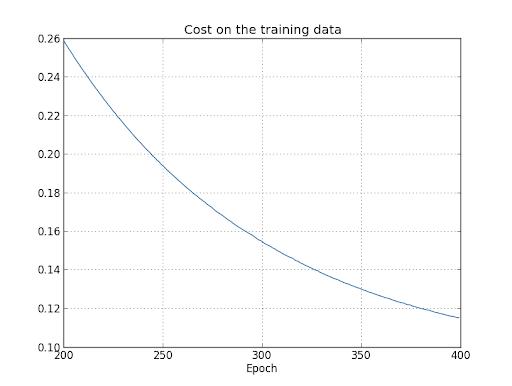
\includegraphics[width = 4in]{Images/Development and Testing/Stage 3/Example Training Curve.png} 
    \label{fig:Example Cost Graph}
\end{figure}
\noindent The code I will use to test is below:
\begin{python}
import numpy as np

# Set the file path of the data
path = "data/train.csv"
width, height = 28,28
pixelCount = width * height

# Load training data
trainingData = np.empty([60000, pixelCount + 1])
row = 0
for line in open(path):
    trainingData[row] = np.fromstring(line, sep=",")
    row += 1

# Used to adjust the greyscale values of the images into the useful interval i.e. between 0 and 1 from the interval 0 - 255
adjust = 0.99 / 255
trainingImages = np.asfarray(trainingData[:, 1:]) * adjust + 0.01

# Getting all the labels in the correct order
trainingLabels = np.asfarray(trainingData[:, :1])
lr = np.arange(10)

# Organising the labels from an identifying float to a one hot representation.
trainingLabelsOneHot = (lr == trainingLabels).astype(np.float)

nn = NeuralNetwork([784, 24, 24, 10], False, "saveFiles/test.txt")
nn.trainNetwork(trainingImages, trainingLabelsOneHot, 1, 0.1, 10)  # starts training the network on data loaded
\end{python}
\noindent One thing that may need explanation is the idea of one-hot encoding. This the idea of representing an integer by the position in an array of 1s and 0s. For example, 3 would become [0, 0, 0, 1, 0, 0] for a number range from 0 - 5. This will be necessary as that is the way the neural network will provide its output.
\newline
I have removed the progress checkups from this output, because it would take up too much space and the final graph summarises all of the checkups much better. The graph that this code outputted is below:
\begin{figure}[H]
    \centering
    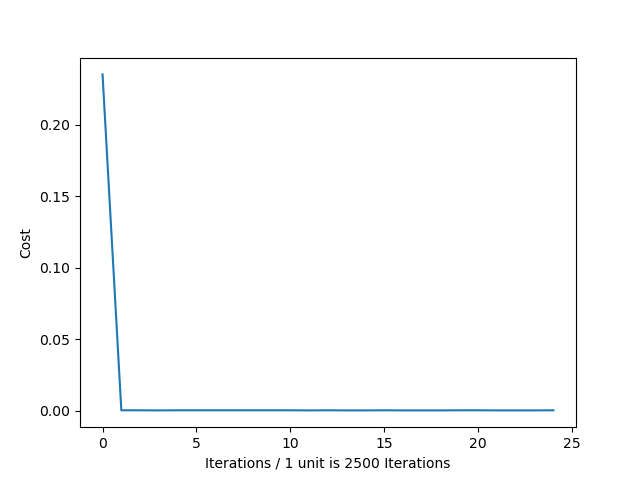
\includegraphics[width = 4in]{Images/Development and Testing/Stage 3/Small Numbers Training Curve.png}
    \label{fig:Small Numbers Cost Graph}
\end{figure}
\noindent The shape of this graph is correct, but the values seem off. This is because in the first 2500 iterations the cost went down to approximately 0, which is extremely low, to the point of impossibility. This means that something is probably wrong with my code. 
\newline
After reading through the code, I realised that there was an error in the \pyth{trainNetwork} function. This line is below: 
\begin{python}
costMean = util.evaluateCost(guess, trueValue)
\end{python}
The problem was that the function was not adding to \pyth{costMean}, so when it was added to the graph, it had become very small (having been divided by 2500). The exception to this was the first iteration, which had a specific if statement, which prevented it from being divided, giving the graph its shape. The solution to this is simple:
\begin{python}
costMean += util.evaluateCost(guess, trueValue)
\end{python}
Running the test code again gave this graph:
\begin{figure}[H]
    \centering
    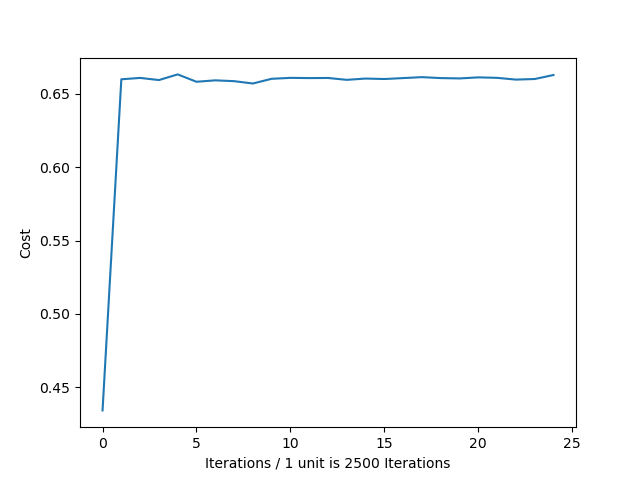
\includegraphics[width = 4in]{Images/Development and Testing/Stage 3/Inverted Training Curve.png} 
    \label{fig:Inverted Cost Graph}
\end{figure}
\noindent This is not at all what I expected to see, instead of the cost decreasing, the cost instead increased rapidly. This means that there will be a negative somewhere in the calculations where there needed to be a positive or vice versa. The two places that this could happen would be in the back-propagation function or the update weights function.
\newline
After combing through the code, I found the source of this error. It is this line in \pyth{backPropagateError()}:
\begin{python}
self.nodes[self.layers - 1][i].error = 2 * (self.nodes[self.layers - 1][i].output - trueValue[i]) * util.sigmoidDerivative(self.nodes[self.layers - 1][i].z) 
\end{python}
The issue with this line is that it sets the error to the gradient of the graph at that point, not the negative of it. This is an issue, as if the error of the node is the same as the gradient, the function will maximise the cost of the network. This means that the error of the node should instead be the negative of the gradient, so it instead minimises the cost. Thus the new code looks like:
\begin{python}
self.nodes[self.layers - 1][i].error = -2 * (self.nodes[self.layers - 1][i].output - trueValue[i]) * util.sigmoidDerivative(self.nodes[self.layers - 1][i].z) 
\end{python}
Running the test code again gave this graph:
\begin{figure}[H]
    \centering
    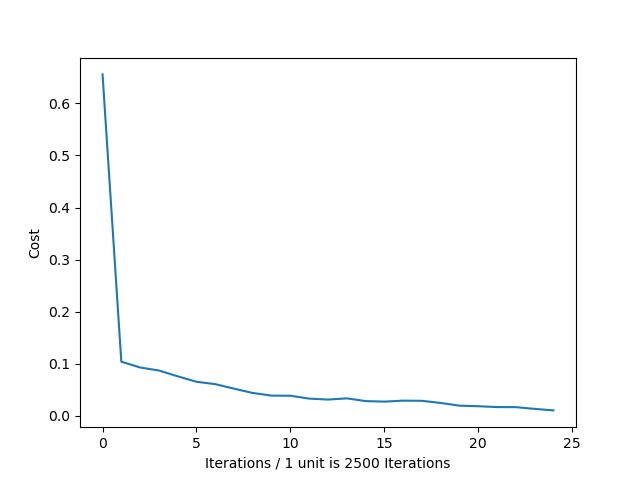
\includegraphics[width = 4in]{Images/Development and Testing/Stage 3/Training Curve.png} 
    \label{fig:Good Cost Graph}
\end{figure}
\noindent This looks much better: there are no values in the graph that look wrong, and the general shape of the graph is similar to the example one shown before. This means that it is quite likely for the network to be working properly. This final test will use \pyth{testNetwork()} to test the network on the testing database provided by MNIST.
\subsection{Testing Function}
This function essentially tests the trained network with unseen data to calculate its accuracy on that test data. The purpose of this function is to be the final check of this section, which checks whether the accuracy of the network is up to scratch and will be useful for the rest of the project. This function will be a simple for loop, which adds up the number of correct guesses, then divides that by the total to get a percentage representing accuracy. The code for this is below:
\begin{python}
def testNetwork(self, testData, testLabels, rightNumber):
    right = 0
    answer = -1
    for i in range(len(testData)):
        self.loadInputs(testData[i])  # load test data into network
        guess = self.feedForward()  # feeds the test data through the network to get an answer
        labels = testLabels[i].tolist()  # converts the label into a list
        correct = labels.index(rightNumber)  # find the value that the label represents
        # loops through the guess array to convert it from a one-hot representation to a single integer
        runningTotal = 0
        for x in guess:
            if x >= runningTotal:
                runningTotal = x
                answer = guess.index(x)
        # checks real answer against guess to determine number of correct guesses
        if correct == answer:
            right += 1
    # Outputs percent accuracy
    print("Total percentage correct:", (right * 100) / len(testData), "%")
\end{python}
Having read through this, there doesn't seem to be any issues with the code. So, the final thing to do is run this function on the network trained in the previous subsection and see what accuracy it achieves. I will again be using the MNIST database to test this network, but I will use the testing database and not the training database. This will ensure that the network has not been trained on the test data. 
\newline
The code I will use to load the previous network and test it is below:
\begin{python}
import numpy as np

# Set the file path of the data
path = "data/test.csv"
width, height = 28,28
pixelCount = width * height

# Load testing data
testingData = np.empty([10000, pixelCount + 1])
row = 0
for line in open(path):
    testingData[row] = np.fromstring(line, sep=",")
    row += 1

# Used to adjust the greyscale values of the images into the useful interval i.e. between 0 and 1 from the interval 0 - 255
adjust = 0.99 / 255
testingImages = np.asfarray(testingData[:, 1:]) * adjust + 0.01

# Getting all the labels in the correct order
testingLabels = np.asfarray(testingData[:, :1])
lr = np.arange(10)

# Organising the labels from an identifying float to a one hot representation
testingLabelsOneHot = (lr == testingLabels).astype(np.float)

nn = NeuralNetwork([784, 24, 24, 10], True, "saveFiles/test.txt")  # load pre-trained network
nn.testNetwork(testingImages, testingLabelsOneHot, 1)  # starts testing the network on data loaded
\end{python}
The output given by running this code is:
\begin{verbatim}
Total percentage correct: 90.29 %
\end{verbatim}
As you can see, the network trained in the previous step, which was only trained for 1 epoch (quite a short time) achieved more than 90\% accuracy on this set of data. This is much higher than guesswork (which would be 10\%), and means that this network is learning correctly and will be accurate enough if trained for longer. As such, the next thing to do will be train the network for a few more epochs and see how much more accurate it becomes.
\newline
After 4 more epochs of training, the network was able to attain an accuracy of 93\% on the test data. This shows that the code written in these stages is bug-free and works as intended.
\newline
The last thing to do is to train the network on a database of normal characters. However, I have not been able to find a suitable character based database, so I will have to post-pone this part and instead use the MNIST database until such a time where I can find a suitable character database. Due to the way I have programmed my network, it should be quite easy to train on any database.
\newpage

\section{Neural Network Review}
This section summarises what has been completed in this section, which success criteria have been completed and any limitations to the current prototype.
\subsection{Features Added}
Quite a few features have been added to the neural network in this section. The list of these features is below:
\begin{itemize}
    \item The neural network can train on wide range of databases and make accurate predictions based on its training from this
    \item The neural network can save its current state to a file
    \item The neural network can load from previously saved to files
    \item The neural network can be of a flexible structure (i.e. number of inputs can change, number of outputs can change or number of hidden nodes can change)
    \item The neural network initialises to a random set of initial conditions
    \item The neural network attains over 90\% accuracy on test data
\end{itemize}
These features will make it easy to integrate the network into the later parts of the program, and will also provide it with the flexibility to be trained by the user on custom data.
\subsection{Success Criteria Fulfilled}
Because this is just the first stage of the project, no success criteria can be fulfilled yet. However, the code written before is a big part in fulfilling the following success criteria:
\begin{itemize}
    \item Ability to train a new network on an users desired database
    \item Ability to use user trained networks
    \item Ability for low-end computers to run it
\end{itemize}
\subsection{Limitations to existing prototype}
At this point, there are only two main limitations to this program. The first is the long run-time of the program. As of now it takes around 40 minutes to fully train the neural network on the MNIST database, and the larger the network/database, the longer it will take to train the network. This may lead to some issues down the line. Another problem is the fact that I have not been able to find a suitable alphabetical character database, meaning that currently the program is limited to translating numerical characters. This may not change, so could become a big issue later on. However, the ability for the user to train the network themselves could bypass this problem. As it stands now, the code for the network is complete and works. This means that when/if I find a suitable database it will be very easy to substitute MNIST for that database.
\newpage

\section{Stage 4 - Simple Image Processing}
In this stage and the next two ones, I will be adding some functions to the utilities library, which will handle image processing and cropping characters out of images. In this stage, I will create the simpler image cleaning algorithms such as ones that remove extraneous noise or the functions that the image tracing algorithms will require. This will then be tested well to ensure no bugs will remain that could cause errors further down the road. I will also be using the PIL library to perform some image manipulation, like compression or for loading images from files.
\subsection{Load images from files}
This is a very simple function that loads an image from a file path, converts it to greyscale and then returns it. The code that I will use for it is below:
\begin{python}
from PIL import Image

def loadImageFromPath(path):
    img = Image.open(path).convert('LA')  # loads image while simultaneously converting it to a greyscale format.
    return img
\end{python}
This code is quite simple. However, I will still test it just to check everything is working correctly. I am going to use the image below as a test image. Next to that image is its location in the folder:
\begin{figure}[H]
    \centering
    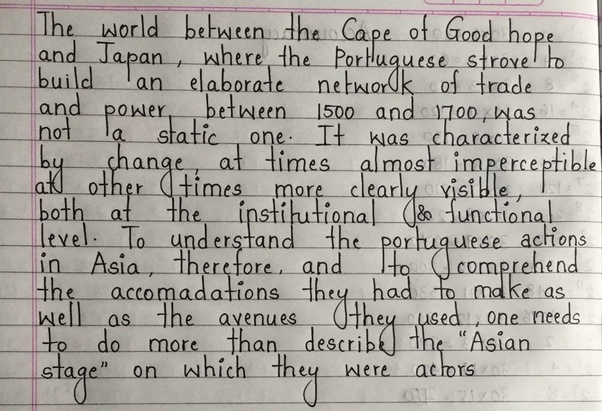
\includegraphics[width = 2.5in]{Images/Development and Testing/Stage 4/Testing for load image from path/testImage1.jpg} 
    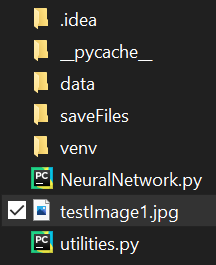
\includegraphics[height = 1.72in]{Images/Development and Testing/Stage 4/Testing for load image from path/ProofOfTestImage.png}
    \label{fig:Test Image}
\end{figure}
\noindent I will then use the test code below to try and load and show the test image:
\begin{python}
img = loadImageFromPath("testImage1.jpg")
img.show()  # This is a inbuilt function to display an image
\end{python}
The output it gave is below:
\begin{figure}[H]
    \centering
    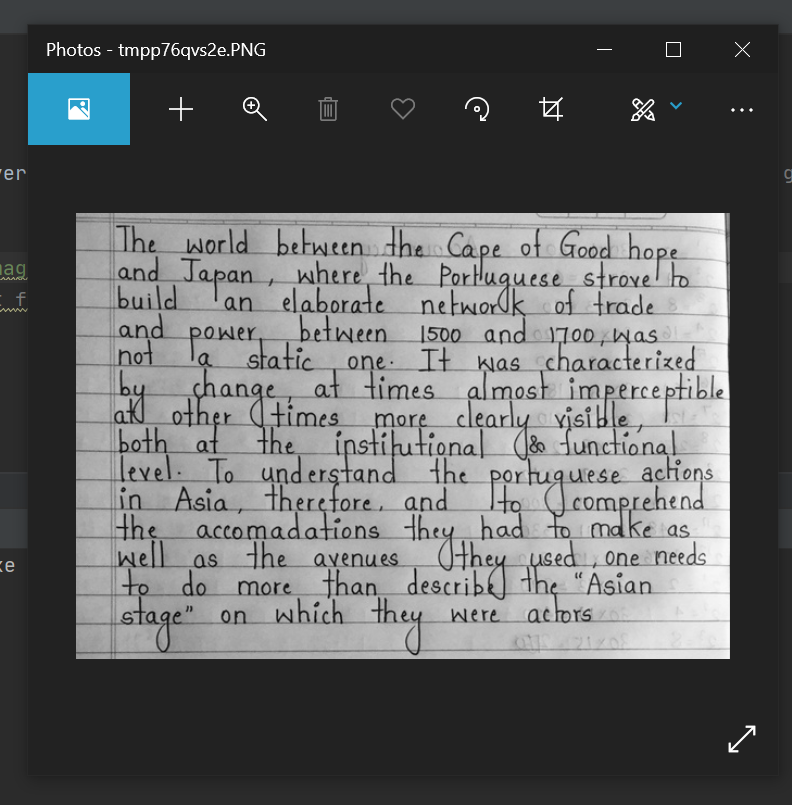
\includegraphics[width = 2.5in]{Images/Development and Testing/Stage 4/Testing for load image from path/Passed Test for Loading from Path.png} 
    \label{fig:Passed Test for Load Image Algorithm}
\end{figure}
\noindent As you can see, the function is working and the color in the image is gone. This means that the function is converting the image to greyscale and loading the image properly.
\subsection{Cleaning the image}
This function will try to remove noise from an input, and then convert that image to an array. The array format is required by the neural network as input. It is slightly more complex as it is difficult to know when something is caused by a shadow and something is just ink. However, I will simply compare how dark a pixel is and then make it completely white if it is below a threshold and leave it unchanged if it above a threshold. I will decide the threshold by calculating the average darkness of each pixel. This will enable photos with different lighting levels to be correctly cleaned. The code for this algorithm is below:
\begin{python}
def cleanImage(img):

    width, height = img.size  # uses inbuilt function to get width and height of image
    average = 0  # initialises average before use
    adjust = 0.99 / 255  # This is an adjust value, which adjust values in the interval 0-255 to the interval 0-0.99
    array = []  # initialises output array before use

    for x in range(width):
        for y in range(height):
            white, black = img.getpixel((x, y))  # Gets the white black balance of a pixel
            average += abs((white - black) * adjust)  # uses the white black balance to calculate a single float that represents how dark a pixel is

    average = average / (width * height) # calculates the average darkness of a pixel

    for x in range(width):
        for y in range(height):
            white, black = img.getpixel((x, y))
            pixelValue = abs((white - black) * adjust)
            if pixelValue > average:  # compares each pixel with the average to see if it needs pruning
                array.append(pixelValue)
            else:
                array.append(0)

    array = np.array(array)
    return array
\end{python}
I will use the following test code to check if the image is being cleaned properly (the image used is the same one as in \textbf{section 3.5.1}):
\begin{python}
img = loadImageFromPath("testImage1.jpg")
img.show()  # shows the image before cleaning
width, height = img.size
img = cleanImage(img)
img = img.reshape((height, width)) # turns the image from a 1d array to a 2d array
plt.imshow(img, cmap="Greys")
plt.show()  # shows the image after cleaning
\end{python}
The output of this program was:
\begin{figure}[H]
    \centering
    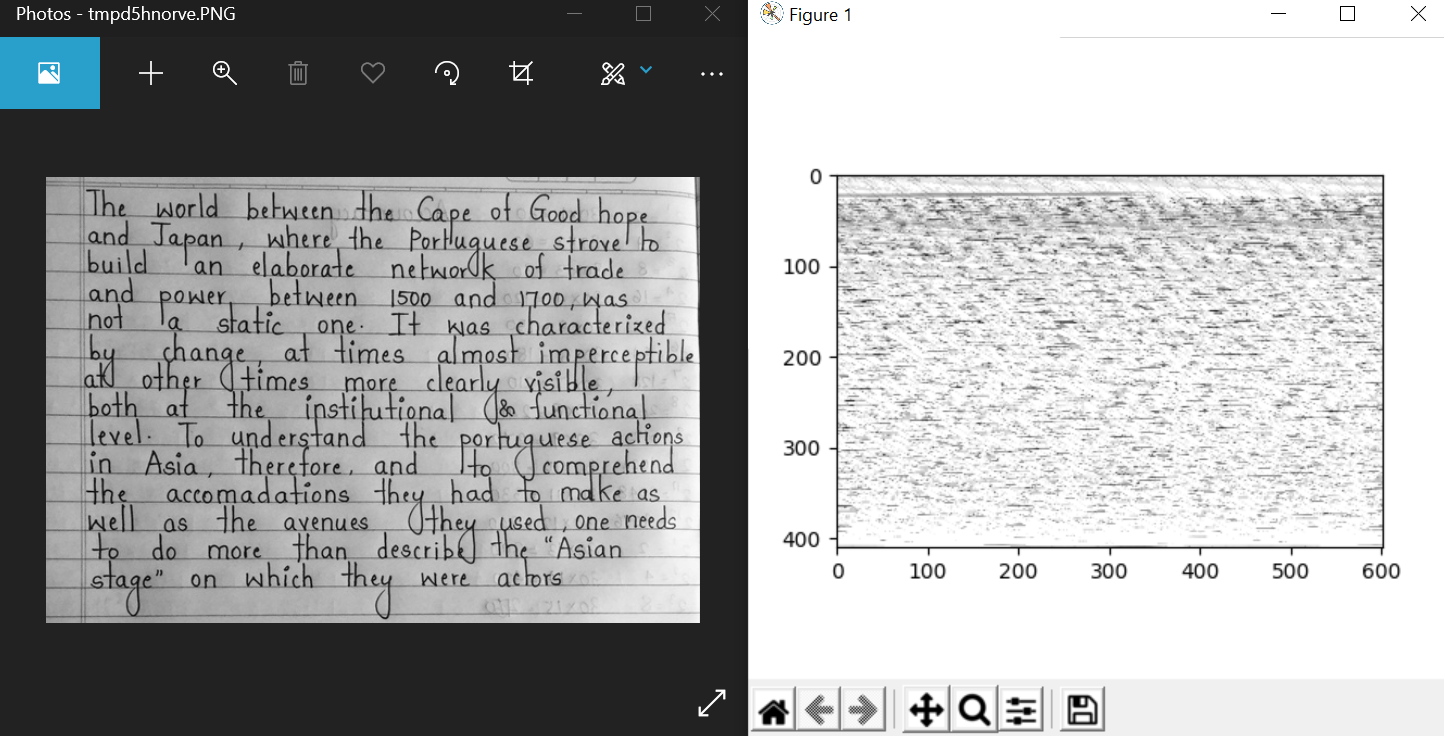
\includegraphics[width=5in]{Images/Development and Testing/Stage 4/Testing for Clean Image/Test 1, Weird Noise.png}
    \label{fig:Testing for Clean Image}
\end{figure}
\noindent The image on the left is the input to the program whereas the image on the right is the output of the function. There is clearly something wrong, making the image look skewed. After reading through the code and performing a few checks, I realised that this error was caused by the way the function was looping through the image. It was iterating through row by row instead of column by column. The new code looks like:
\begin{python}
def cleanImage(img):

    width, height = img.size  # uses inbuilt function to get width and height of image
    average = 0  # initialises average before use
    adjust = 0.99 / 255  # This is an adjust value, which adjust values in the interval 0-255 to the interval 0-0.99
    array = []  # initialises output array before use

    for y in range(height):
        for x in range(width):
            white, black = img.getpixel((x, y))  # Gets the white black balance of a pixel
            average += abs((white - black) * adjust)  # uses the white black balance to calculate a single float that represents how dark a pixel is

    average = average / (width * height) # calculates the average darkness of a pixel

    for y in range(height):
        for x in range(width):
            white, black = img.getpixel((x, y))
            pixelValue = abs((white - black) * adjust)
            if pixelValue > average:  # compares each pixel with the average to see if it needs pruning
                array.append(pixelValue)
            else:
                array.append(0)

    array = np.array(array)
    return array
\end{python}
Now rerunning the testing code gives:
\begin{figure}[H]
    \centering
    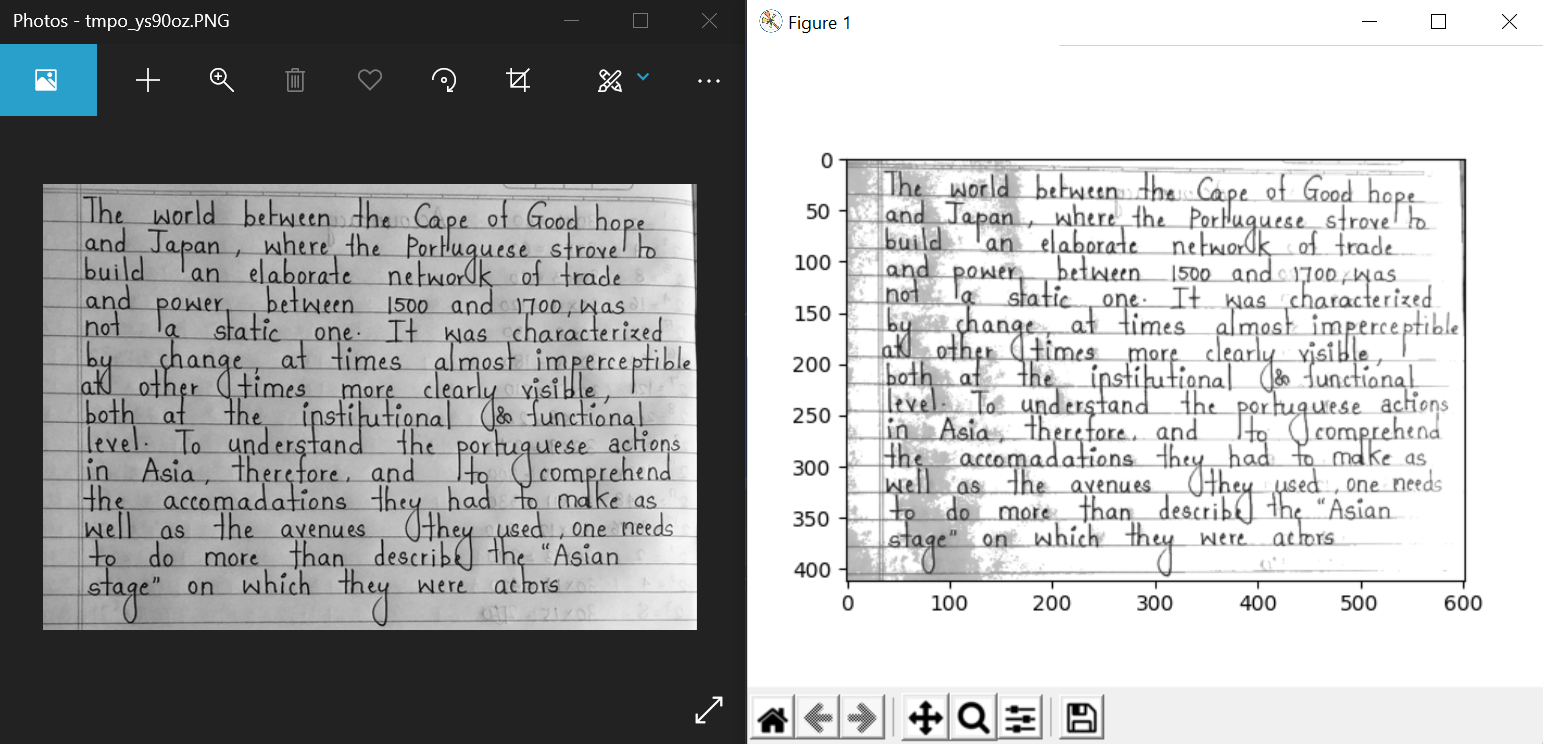
\includegraphics[width=5in]{Images/Development and Testing/Stage 4/Testing for Clean Image/Test 2, Too much noise.png}
    \label{fig:Testing for Clean Image: Test 2}
\end{figure}
\noindent Again, the input to the function is on the left while the output is on the right. This is an improvement over the previous output, as the image is now legible. However there is still a lot of noise, the lines are still visible and there are noticeable shadows on the left of the output image. Clearly the threshold for making pixels white is too low and is allowing noise over the threshold. I realised a good fix for this would be to multiple the average by a scalar to obtain the threshold. I will determine the scalar by changing it and seeing which image gives the least amount of noise for clarity.
\newline
Through more testing I found that near ideal constant was ~ 1.9. Making the change in this line:
\begin{python}
if pixelValue > average:  # compares each pixel with the average to see if it needs pruning
\end{python}
I simply changed it to:
\begin{python}
if pixelValue > average * 1.9:  # compares each pixel with a scalar multiple of the average to see if it needs pruning
\end{python}
The output I got from rerunning the testing code is now:
\begin{figure}[H]
    \centering
    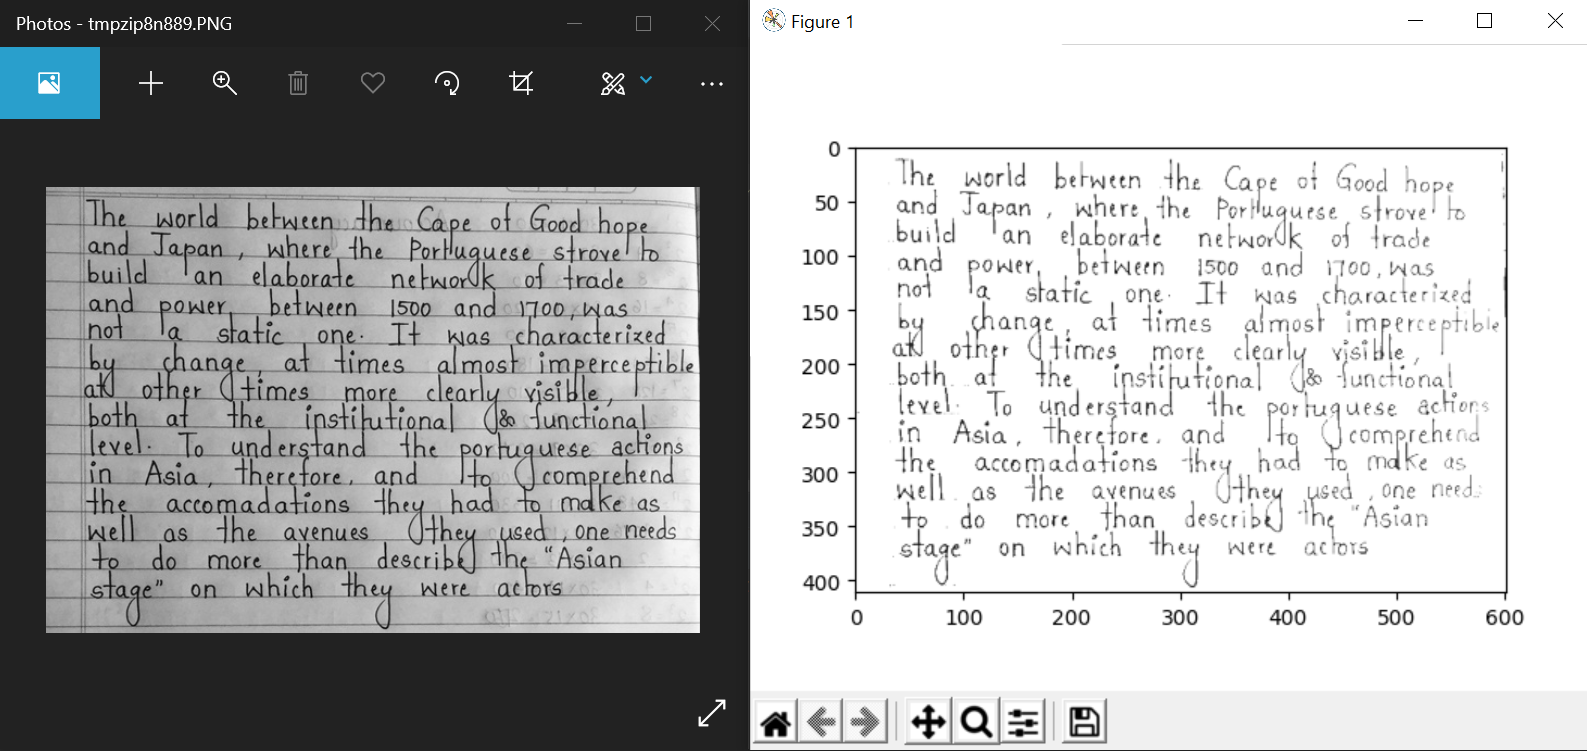
\includegraphics[width=5in]{Images/Development and Testing/Stage 4/Testing for Clean Image/Test 3, Looks Good.png}
    \label{fig:Testing for Clean Image: Test 3}
\end{figure}
\noindent Again the input to the function is on the left while the output is on the right. As you can see the output looks very good, with almost no noise apart from a few small dots scattered about. These can however be easily removed later on because they are so small. In addition, the actual image has not lost much useful information. There is only one loss which is the 's' at the end of 'needs' on the third last line of the image. However this is still not too bad as a small loss of information is worth the removal of all noise.
\newline
As a final test of this function, I will run it on a different sample of handwriting, below:
\begin{figure}[H]
    \centering
    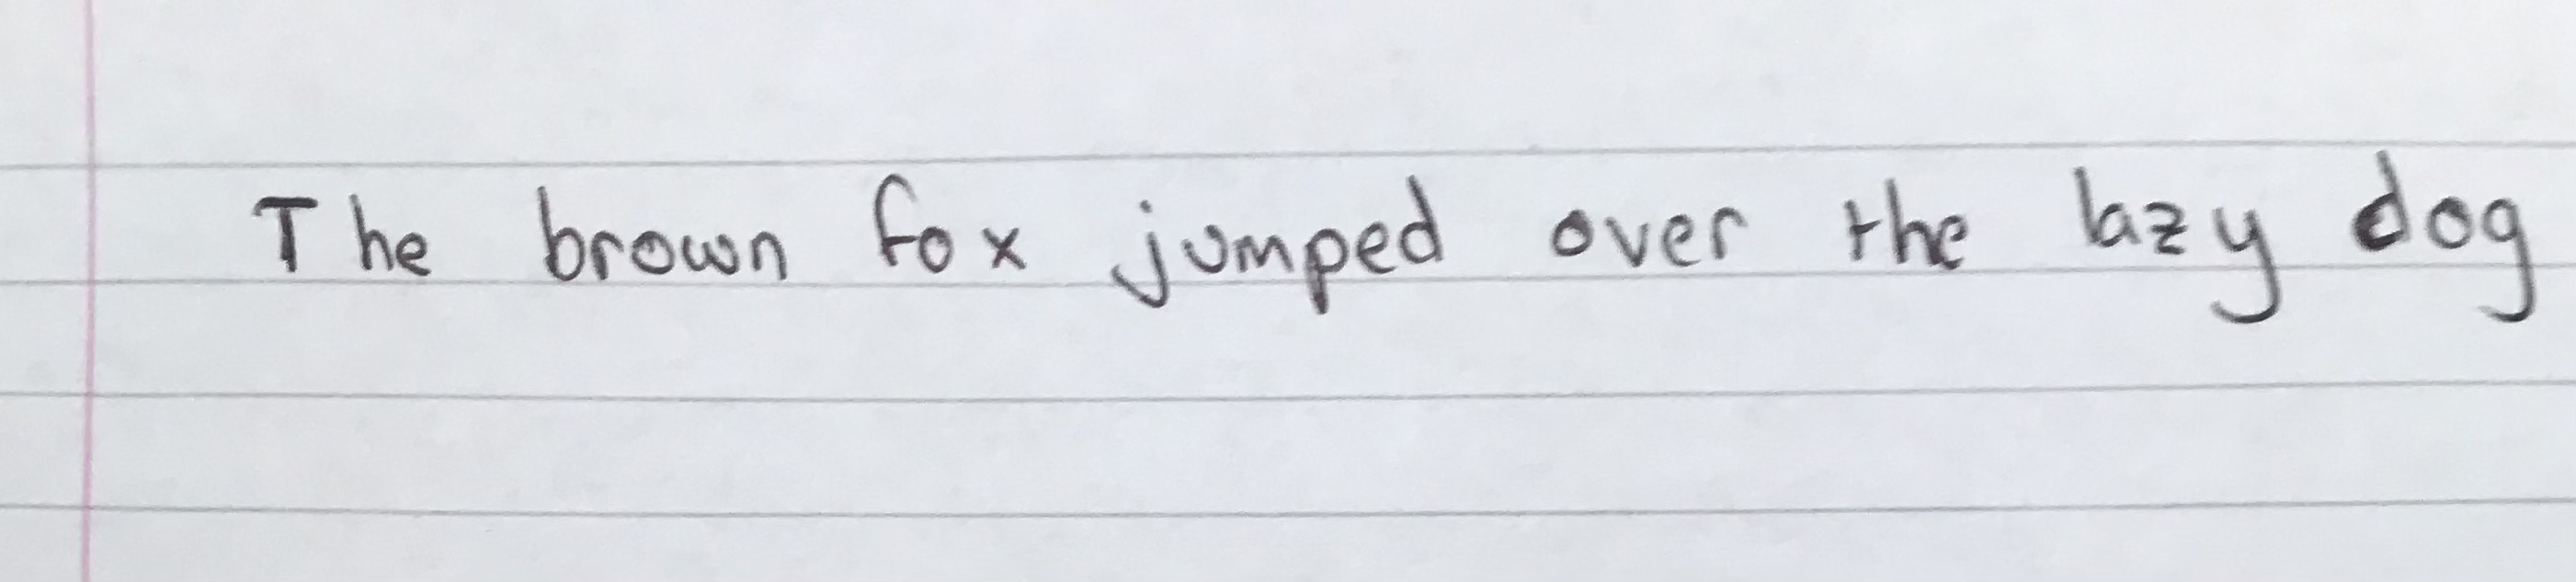
\includegraphics[height=1in]{Images/Development and Testing/Stage 4/Testing for Clean Image/testImage2.jpg}
    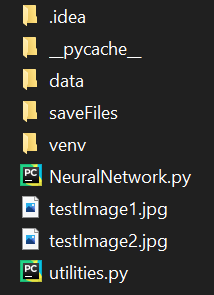
\includegraphics[height=1in]{Images/Development and Testing/Stage 4/Testing for Clean Image/ProofOfTestImage2.png}
    \label{fig:Final Test data for Clean Image}
\end{figure}
\noindent On the left is the image and on the right is the location in the file system.
\newline
A quick change to the testing code to make it load the new test image and the test is good to run:
\begin{python}
img = loadImageFromPath("testImage2.jpg")
img.show()
width, height = img.size
img = cleanImage(img)
img = img.reshape((height, width))
plt.imshow(img, cmap="Greys")
plt.show()
\end{python}
The output this code now gives is:
\begin{figure}[H]
    \centering
    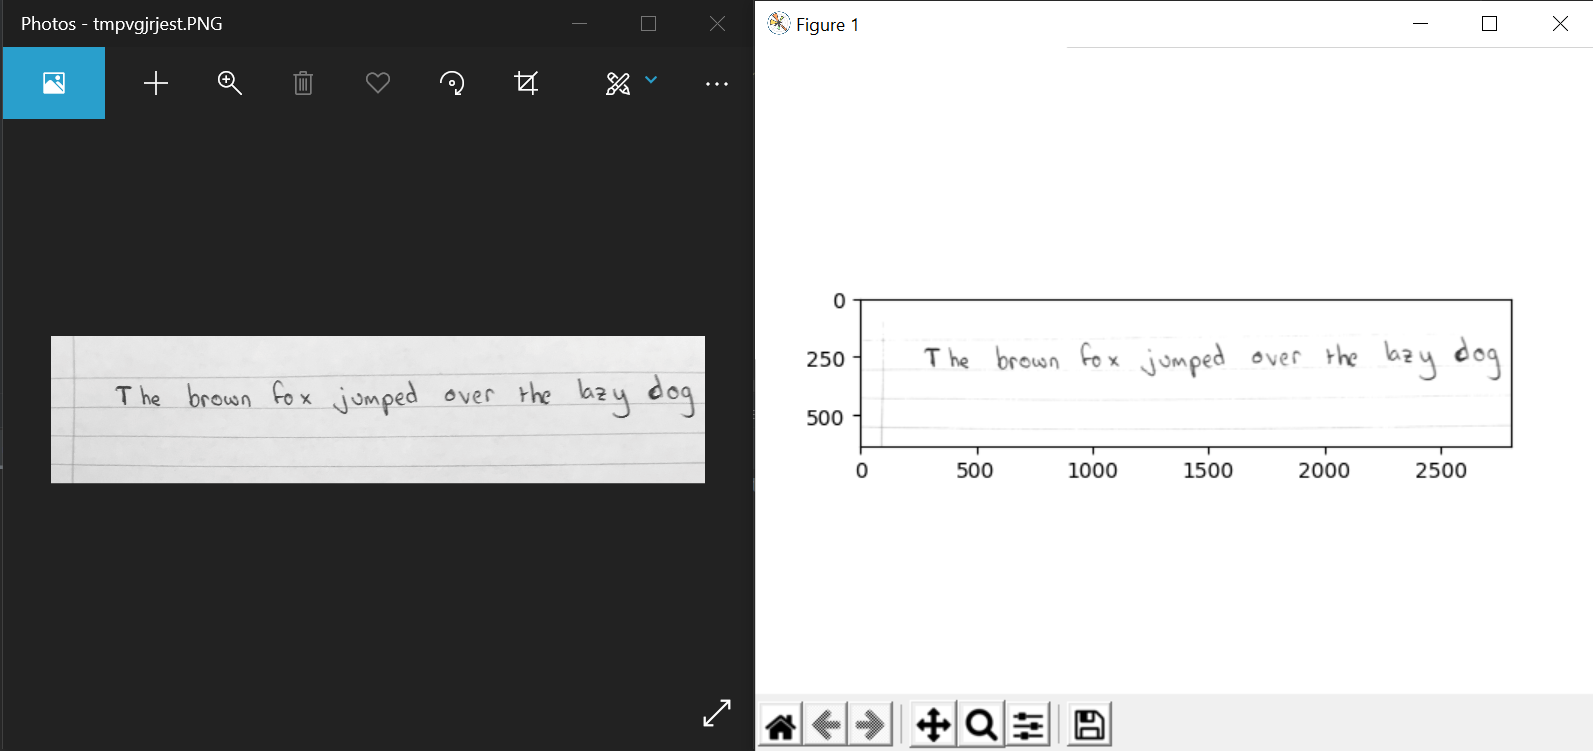
\includegraphics[width=5in]{Images/Development and Testing/Stage 4/Testing for Clean Image/Test 4, Did not work.png}
    \label{fig:Testing Clean Image: Test 4}
\end{figure}
\noindent As you can see, the code did not work well for this image. The issue is that again the threshold is too low so the scalar will have to change again. This means that the scalar is in fact a variable and will have to change with the value of average.
\newline
After performing more tests, I realised that in this particular case, the value of the scalar needs to be bigger. Since the average is smaller than with the other test image I hypothesised that the scalar and the average were inversely proportional and postulated the equation $y = c + a/x$ where $y$ is the scalar and $x$ is the average. I could then use the correct values I had found for $y$ and $x$ in each previous case to solve simultaneous equations and find $a = 1.534$ and $c = 0.1251$. This gave the equation $y = 1.534 + 0.1251/x$ which I was confident would work. 
\newline
The next step, after implementing this was to use another random handwriting sample and test the new code on that to see if it works. The code I changed was this line:
\begin{python}
if pixelValue > average * 1.9:  # compares each pixel with a scalar multiple of the average to see if it needs
\end{python}
I changed it to this:
\begin{python}
if pixelValue > average * (1.534 + 0.1251/average):  # compares each pixel with a multiple of the average to see if it needs pruning
\end{python}
I then used this test image (with the location of it in the file system shown to the right) as a check that this new code would work:
\begin{figure}[H]
    \centering
    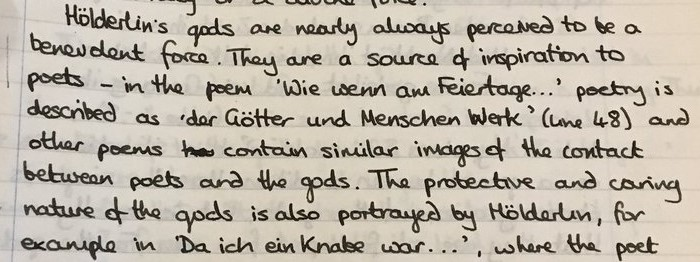
\includegraphics[height=1.5in]{Images/Development and Testing/Stage 4/Testing for Clean Image/testImage3.jpg}
    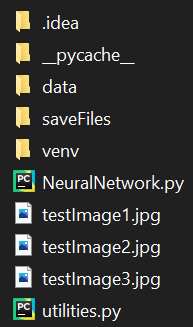
\includegraphics[height=1.5in]{Images/Development and Testing/Stage 4/Testing for Clean Image/ProofOfTestImage3.png}
    \label{fig:Test Image 3 and location}
\end{figure}
\noindent The code I used to perform the test is below:
\begin{python}
img = loadImageFromPath("testImage3.jpg")
img.show()
width, height = img.size
img = cleanImage(img)
img = img.reshape((height, width))
plt.imshow(img, cmap="Greys")
plt.show()
\end{python}
The result of running this code was:
\begin{figure}[H]
    \centering
    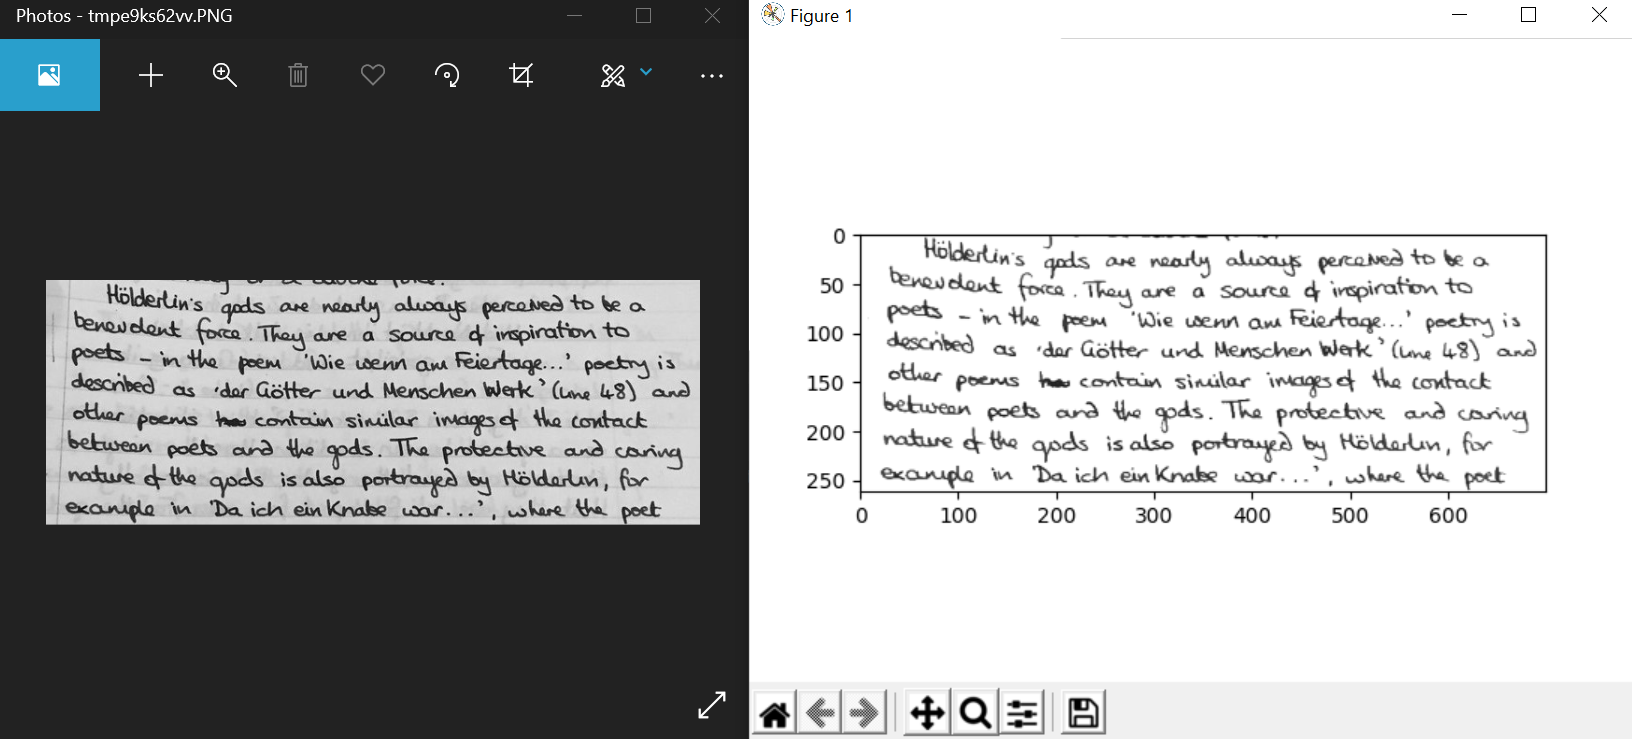
\includegraphics[width=5in]{Images/Development and Testing/Stage 4/Testing for Clean Image/Test 5, Working Now.png}
    \label{fig:Clean Image: Final Test}
\end{figure}
\noindent As you can see, this code is working well now and is fully cleaning a variety of images and converting into the proper data type for the program. Thus this function is good and safe to be used later on down the line. So the final code for the clean image function is:
\begin{python}
def cleanImage(img):

    width, height = img.size  # uses inbuilt function to get width and height of image
    average = 0  # initialises average before use
    adjust = 0.99 / 255  # This is an adjust value, which adjust values in the interval 0-255 to the interval 0-0.99
    array = []  # initialises output array before use

    for y in range(height):
        for x in range(width):
            white, black = img.getpixel((x, y))  # Gets the white black balance of a pixel
            average += abs((white - black) * adjust)  # uses the white black balance to calculate a single float that represents how dark a pixel is

    average = average / (width * height) # calculates the average darkness of a pixel
    print(average)
    for y in range(height):
        for x in range(width):
            white, black = img.getpixel((x, y))
            pixelValue = abs((white - black) * adjust)
            if pixelValue > average * (1.534 + 0.1251/average):  # compares each pixel with a multiple of the average to see if it needs pruning
                array.append(pixelValue)
            else:
                array.append(0)

    array = np.array(array)
    return array
\end{python}
After making this final function, I realised that there was no need to convert the image into an array at this stage. So I decided to remove that from this function and separate that feature into a different function which I will code next. The new code therefore looks like:
\begin{python}
def cleanImage(img):
    width, height = img.size  # uses inbuilt function to get width and height of image
    average = 0  # initialises average before use
    adjust = 0.99 / 255  # This is an adjust value, which adjust values in the interval 0-255 to the interval 0-0.99
    for y in range(height):
        for x in range(width):
            white, black = img.getpixel((x, y))  # Gets the white black balance of a pixel
            average += abs((white - black) * adjust)  # uses the white black balance to calculate a single float that represents how dark a pixel is
    average = average / (width * height) # calculates the average darkness of a pixel
    for y in range(height):
        for x in range(width):
            white, black = img.getpixel((x, y))
            pixelValue = abs((white - black) * adjust)
            if pixelValue < average * (1.534 + 0.1251/average):  # compares each pixel with a multiple of the average to see if it needs pruning
                img.putpixel((x, y), (255, 255))  # changes the pixel to white
    return img
\end{python}
\subsection{Convert Image to Array}
For this algorithm, I will essentially re-purpose the code I removed from the previous function which was used to convert the image into an array after cleaning. I am putting this into its own function because I will need to convert the image to an array only right before inputting it into the neural network and I will need to clean the image of noise before doing anything with it. This means that these two functions need to be split up into separate ones. The code for this function is below:
\begin{python}
def convertImageToArray(img):
    width, height = img.size  # initialises the width and to that of the image
    adjust = 0.99 / 255  # this will be used to change all the pixel values from the range 0 - 255 to the range 0 - 0.99
    output = []  # initialises the output array to allow appending

    for y in range(height):
        for x in range(width):
            white, black = img.getpixel((x, y))  # gets the white, black balance of an image
            output.append(abs(white - black) * adjust)  # appends the pixel colour now in the range 0-0.99 to the array

    output = np.array(output)
    return output
\end{python}
I used the following test code to check whether the input image was correctly transformed into an array.
\begin{python}
img = loadImageFromPath("testImage2.jpg")
img.show()
width, height = img.size
img = convertImageToArray(img)
img = img.reshape((height, width))
plt.imshow(img, cmap="Greys")
plt.show()
\end{python}
The output running this code gave was:
\begin{figure}[H]
    \centering
    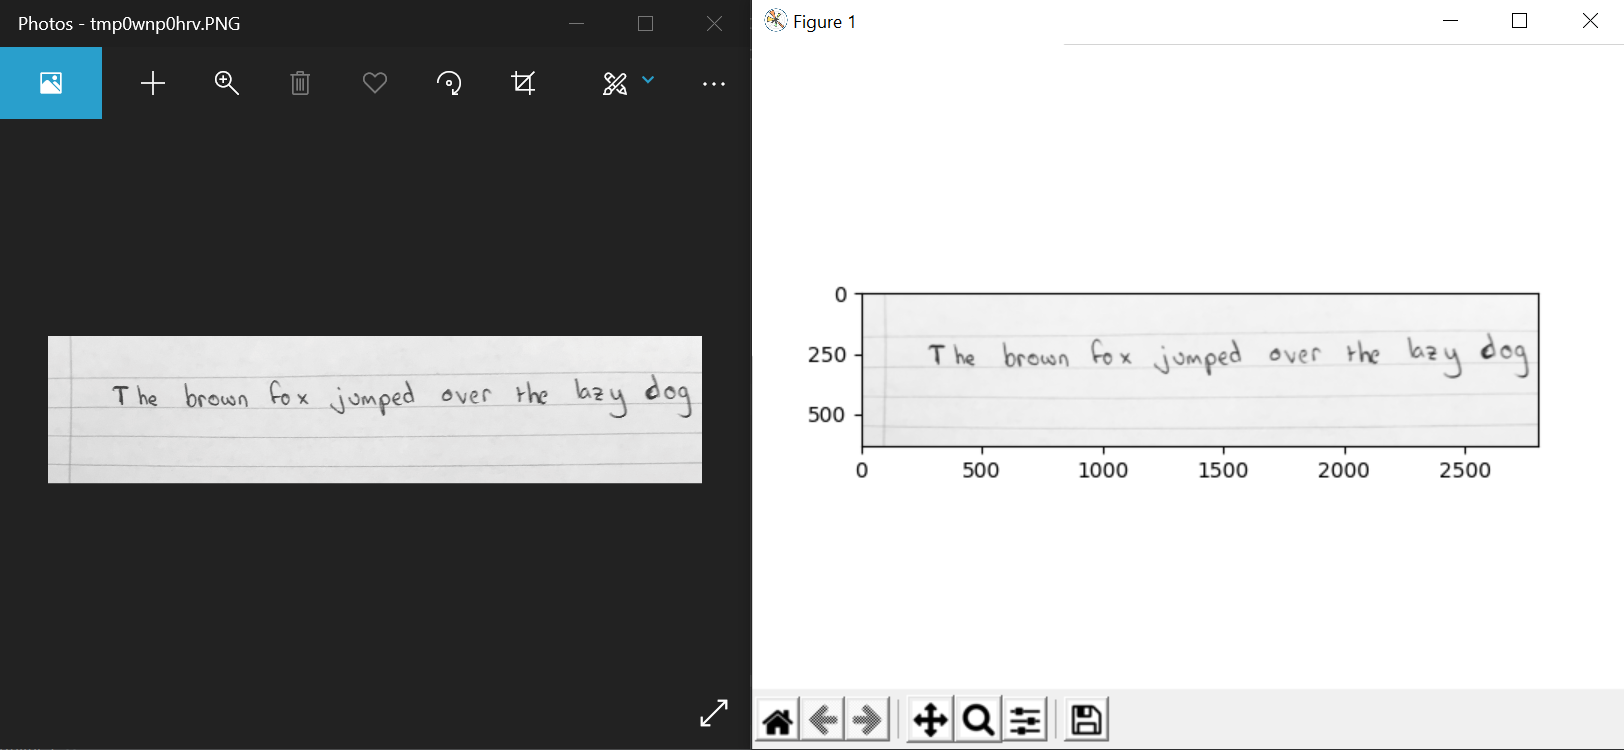
\includegraphics[width=4in]{Images/Development and Testing/Stage 4/Testing For Convert Image To Array/Test 1.png}
    \label{fig:Convert Image To Array: Test 1}
\end{figure}
\noindent As you can see, there were no errors when running this function and the image was converted successfully.
\subsection{Find Boundaries of Image}
This function will find the boundary points of an image. It will find the x co-ordinate of the farthest right and left pixel as well as the y co-ordinate of the highest and lowest pixel in an image. This will enable me to correctly crop out images from a large amount of pixels or centre those images to make it easier for the network to predict the answer. The code for this function is below:
\begin{python}
def findBoundaryBox(img):

    width, height = img.size  # stores width and height of image in two variables
    left = float("inf")  # sets left to infinity
    right = 0  # sets right to 0
    top = float("inf")  # sets top to infinity
    bottom = 0  # sets bottom to 0

    # Loops through the image to find the bottom, right-hand side, left-hand side and top of the image
    for y in range(height):
        for x in range(width):
            white, black = img.getpixel((x, y))  # Gets the white, black composition of the pixel at the current (x, y)
            if (white, black) != (255, 255):  # Checks if pixel is coloured
                # finds the top by checking if the current pixels y value is lower (higher) that the running total
                # the same method is used to find the bottom but in reverse
                if y <= top:
                    top = y
                if y >= bottom:
                    bottom = y

                # finds the left by checking if the current pixels x value is lower (to the left) that the running total
                # the same method is used to find the right but in reverse
                if x <= left:
                    left = x
                if x >= right:
                    right = x

    return left, top, right, bottom
\end{python}
I am going to test this function by inputting a small image with 32x32 pixels that I can count individually, to check that the programs output is correct. The image that I will input is below:
\begin{figure}[H]
    \centering
    
\includegraphics[height = 1in]{Images/Development and Testing/Stage 4/Find Bounding Box Testing/Test Image.png}
    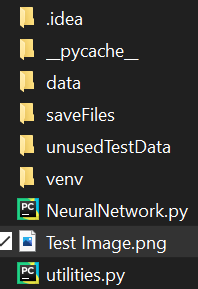
\includegraphics[height = 1in]{Images/Development and Testing/Stage 4/Find Bounding Box Testing/Test Image in File System.png}
    \label{fig:Test Image for Boundary Finder}
\end{figure}
\noindent Now, I will put a scale on the image to enable me to count the x co-ordinates of the right and left and count the y co-ordinates of the top and bottom which I can then check against the programs output.
\newline
The scale that I drew on the image is below:
\begin{figure}[H]
    \centering
    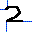
\includegraphics[height = 1in]{Images/Development and Testing/Stage 4/Find Bounding Box Testing/Test Image with scale drawn on.png}
    \label{fig:Test Image with Scale}
\end{figure}
\noindent Using this scale I calculated that the correct values are as follows:
\newline
left - 5
\newline
top - 6
\newline
right - 22
\newline
bottom - 21
\newline
I then used the python code below to utilise the function I created to try and get the same values for the same input image:
\begin{python}
img = loadImageFromPath("Test Image.png")
left, top, right, bottom = findBoundaryBox(img)
print("Left - ", left)
print("Right - ", right)
print("Top - ", top)
print("Bottom - ", bottom)
\end{python}
The output i got after running this code was:
\begin{verbatim}
Left -  5
Right -  22
Top -  6
Bottom -  21
\end{verbatim}
These results are as expected, meaning there are no issues with the function.
\newpage
\subsection{Centre Image}
The purpose of this function will be to ensure any outputted images at the end of the are properly centred and thus will not cause issues with the neural network as the network has been trained on centred images and not on images that haven't been centered properly. I will use the \pyth{findBoundaryBoxFunction(img)} to find the boundaries of the image, which I will then use to crop out the image and paste it into a new image in the centre of that image. The code for the function is below:
\begin{python}
def centreImage(img):

    width, height = img.size  # get the width and height of image
    left, top, right, bottom = findBoundaryBox(img)  # uses the previous function created to find the boundary of the image
    tgtImg = Image.new('LA', (width, height))  # creates a new greyscale image with the same dimensions as the input
    # the for loop below ensures that the image has white pixels to start off with instead of being see-through
    for x in range(width):
        for y in range(height):
            if tgtImg.getpixel((x, y)) == (0, 0):
                tgtImg.putpixel((x, y),(255, 255))

    img = img.crop((left, top, right + 1, bottom + 1))  # crops out the bounded stuff in the image
    # this places the stuff that got cropped out into the image at the correct (x, y) using some simple maths
    tgtImg.paste(img, (int((width / 2) - (right - left) / 2), int((height / 2) - (bottom - top) / 2)))

    return tgtImg  # returns the newly created image
\end{python}
I will test this function by providing it with some images that have not been centred and then seeing whether it is able to centre them. The images I will use and their locations in the file system are below:
\begin{figure}[H]
    \centering
    \fbox{
\includegraphics[height = 1.5in]{Images/Development and Testing/Stage 4/Centre Image/Corner Test Image.png}}    
    \fbox{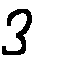
\includegraphics[height = 1.5in]{Images/Development and Testing/Stage 4/Centre Image/Real Test Image.png}}
    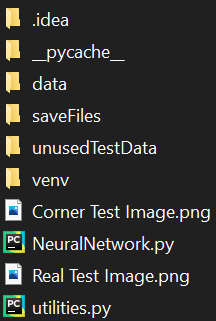
\includegraphics[height = 1.5in]{Images/Development and Testing/Stage 4/Centre Image/Location in File System.png}
    \label{fig:input images}
\end{figure}
\noindent The code I will use to test the function is below:
\begin{python}
img = loadImageFromPath("Corner Test Image.png")  # load test image from path
img.show()  # display starting image
img = centreImage(img)  # centre image
img.show()  # display output image
\end{python}
The output the function gave is below, with the input image shown on the left and the output image shown  on the right.
\begin{figure}[H]
    \centering
    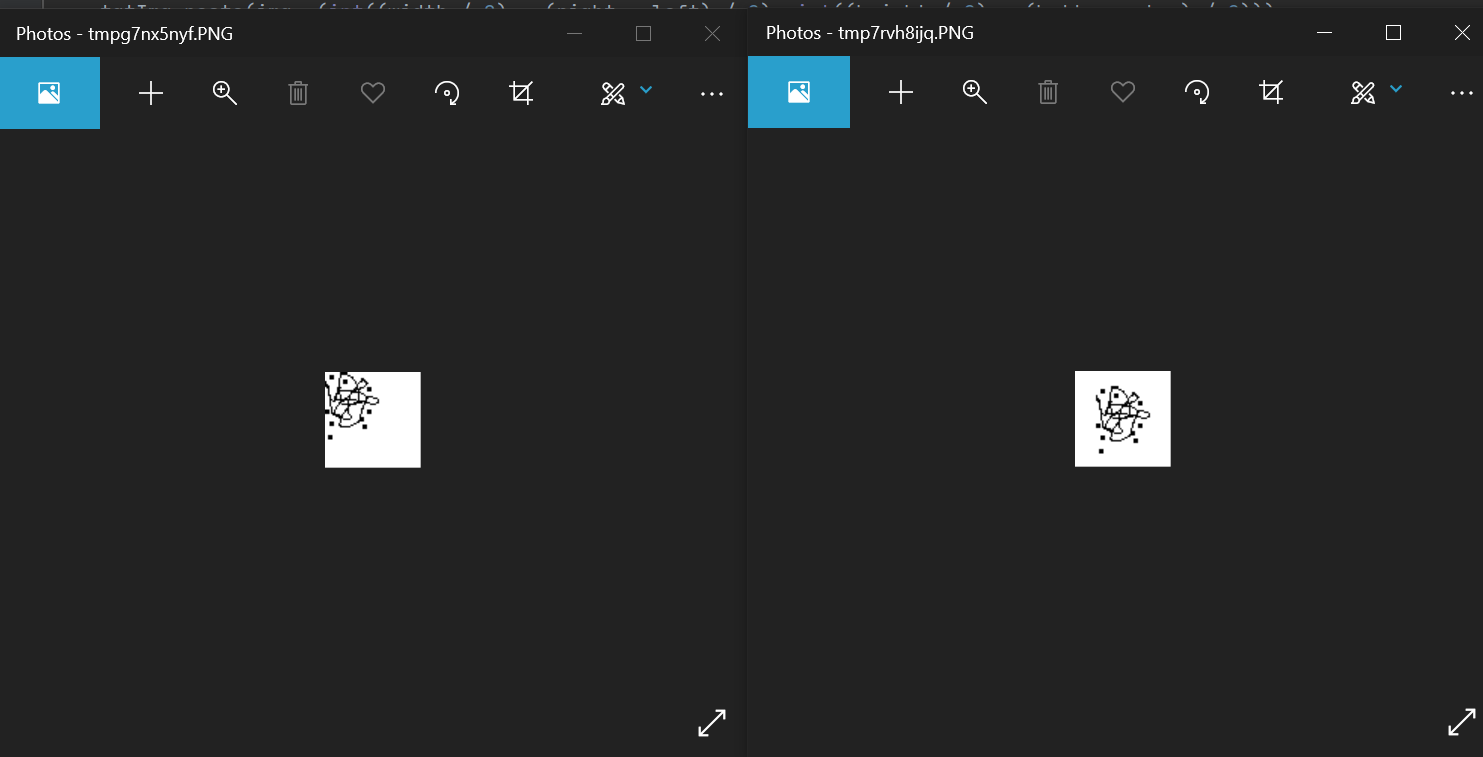
\includegraphics[height=1.5in]{Images/Development and Testing/Stage 4/Centre Image/Corner Test Image - Test.png}
    \label{fig:Test-Corner Case}
\end{figure}
\begin{figure}[H]
    \centering
    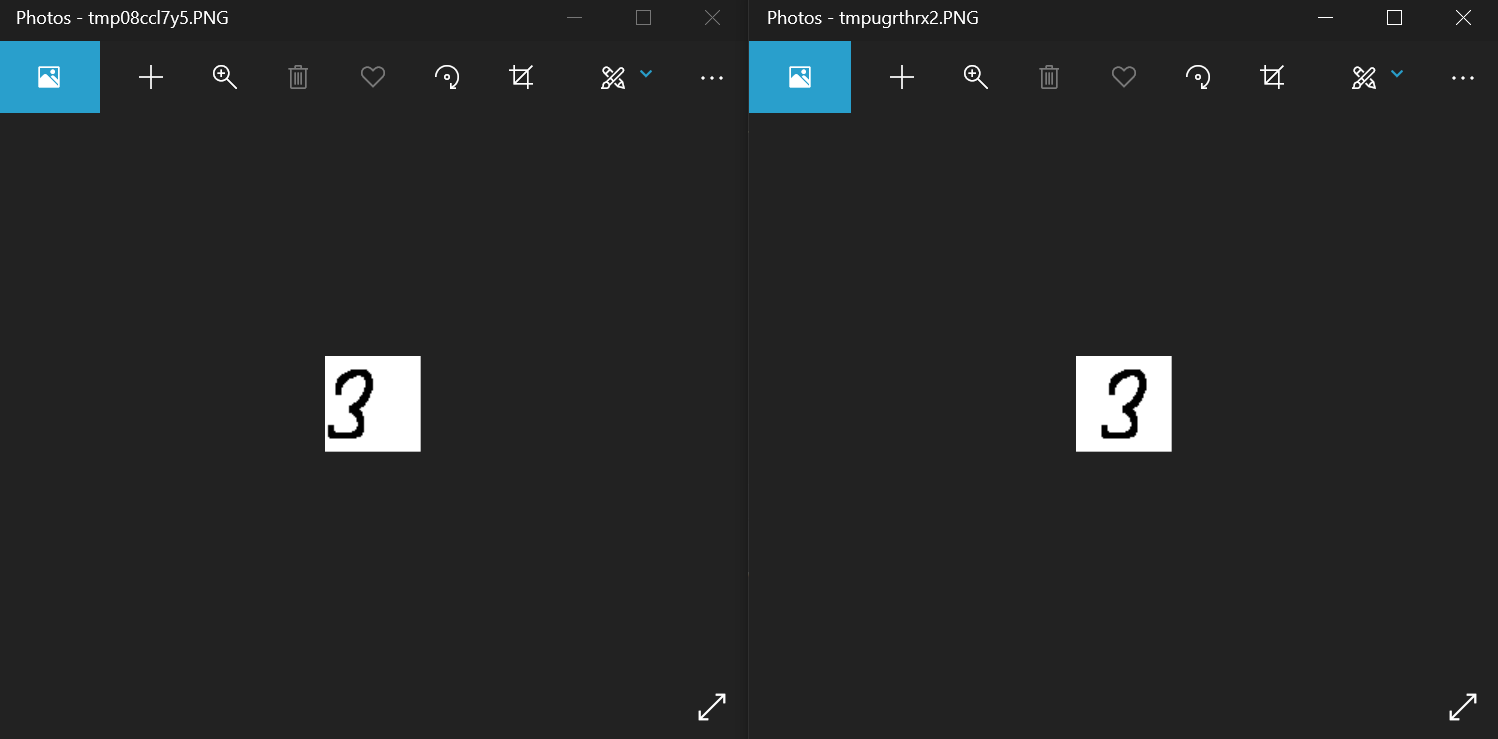
\includegraphics[height=1.5in]{Images/Development and Testing/Stage 4/Centre Image/Real Test Image - Test.png}
    \label{fig:Test-Real Image Case}
\end{figure}
\noindent As you can see, the function is working correctly and is properly centering each image. In addition, there is no lost data around the edges, which is what I was worried about, because there may have been an off by one error in \pyth{findBoundaryBox()}. However this issue has not presented itself so all is well.
\newline
The completion of this function concludes the first stage of the character tracing segment. Now that all of the necessary functions are in place, I will be able to move onto implementing my own character tracing algorithm.
\newpage
\section{Stage 5 - Character Tracing Algorithm}
This section is where I will begin to code the algorithm for cutting a character out of a larger image with nothing else in it. My plan for this is to create an algorithm that starts at a random point on the edge of the image and then jumps to adjacent squares according to a priority list, implemented in the form of a few if statements. To show the different priorities I will make use of a diagram shown below:
\begin{figure}[H]
    \centering
    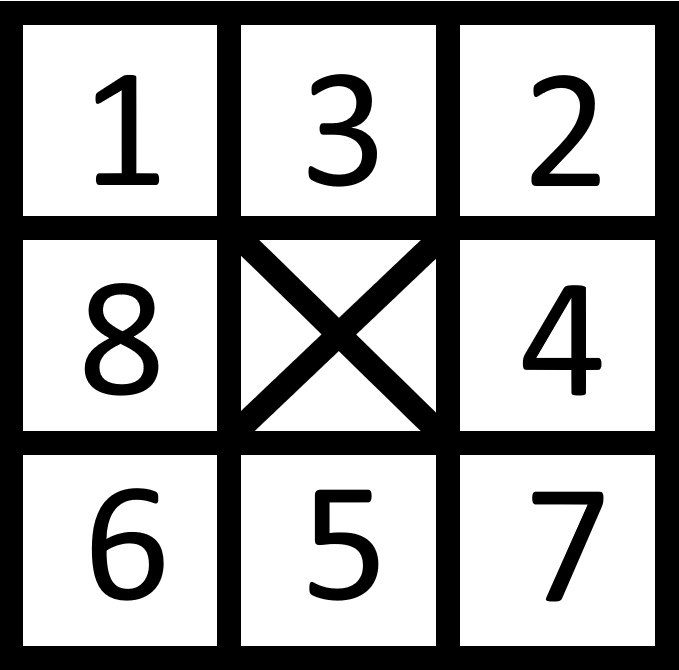
\includegraphics[height = 1.5in]{Images/Development and Testing/Stage 5/Priority Square Example.png}
    \caption{This is an example table}
    \label{fig:Example Priority Square}
\end{figure}
\noindent The crossed out square in the centre represents of pixel that is currently selected by the program. The squares surrounding the crossed square represent the adjacent pixels to the currently selected pixels. The numbers in these squares show the next pixel that the program will attempt to jump to, prioritising the lower numbers. 
\newline
For example, the program will attempt to jump to the square labelled "1", if this pixel is not colored, it will instead attempt to jump to square "2" and so on. The program will also keep count of the pixels it's been to, and will not jump to a pixel that it has already been to. The program will then stop if there are no possible adjacent pixels for it to jump to.
\newline
The program can then use the list of pixels it has gotten that it knows are part of the image to find the boundaries of the image to then crop out the image from the starting image.
\newline
This process will enable me to separate out every shape in an input image to then pass individually through the network. It will also allow me to remove any final noise from the image by checking how small the shape that has been cut out is. The testing process for this function will consist of postulating different possibilities for priorities and seeing how well they work with a variety of input images.
\newline
The testing images images that I will use are below:
\begin{figure}[H]
    \centering
    \fbox{
\includegraphics[height = 0.9in]{Images/Development and Testing/Stage 5/Test Images/8 - number test image.png}}
    \fbox{
\includegraphics[height = 0.9in]{Images/Development and Testing/Stage 5/Test Images/a - letter test image.png}}
    \fbox{
\includegraphics[height = 0.9in]{Images/Development and Testing/Stage 5/Test Images/m - letter test image.png}}
    \fbox{
\includegraphics[height = 0.9in]{Images/Development and Testing/Stage 5/Test Images/f - letter test image.png}}
    \fbox{
\includegraphics[height = 0.9in]{Images/Development and Testing/Stage 5/Test Images/o - letter test image.png}}
    \label{fig:Test Images}
\end{figure}
\noindent As you can see there is a variety of different geometric shapes included in these images that will be difficult for the program to handle and will enable effective testing and improvement of the program.
\newpage
\noindent Below is the code implementing the priority square above: 
\begin{python}
def cropOutCharacter(x, y, img):
    
    width, height = img.size  # Initialise width and height to correct value
    characterFound = False  # This boolean will be used to ensure the while loop below properly exits
    tgtImg = Image.new('LA', (width, height))  # This initialises an empty greyscale image of the same dimensions as the input
    for a in range(width):
        for b in range(height):
            tgtImg.putpixel((x, y), (255, 255))  # Simply sets all the pixels in the image to white pixels
    
    # loops until character is found
    while not characterFound:

        tgtImg.putpixel((x, y), (img.getpixel((x, y))))  # adds the current pixel to tgtImg, to allow graphical representation of pixels visited
        img.putpixel((x, y), (255, 255))  # replaces the current pixel with a white pixel, so there won't be any duplicates

        #  these if statements prevent index out of bounds error
        if x == 0:
            x += 1
        if y == 0:
            y += 1
        if x == width - 1:
            x = width - 2
        if y == height - 1:
            y = height - 2
        
        # The following if statements implement a priority square
        
        # Direction 1
        if img.getpixel((x-1, y-1)) != (255, 255):
            x -= 1
            y -= 1
        # Direction 7
        elif img.getpixel((x+1, y-1)) != (255, 255):
            x += 1
            y -= 1
        # Direction 8
        elif img.getpixel((x, y-1)) != (255, 255):
            y -= 1
        # Direction 6
        elif img.getpixel((x+1, y)) != (255, 255):
            x += 1
        # Direction 4
        elif img.getpixel((x, y+1)) != (255, 255):
            y += 1
        # Direction 3
        elif img.getpixel((x-1, y+1)) != (255, 255):
            x -= 1
            y += 1
        # Direction 5
        elif img.getpixel((x+1, y+1)) != (255, 255):
            x += 1
            y += 1
        # Direction 2
        elif img.getpixel((x-1, y)) != (255, 255):
            x -= 1
        else:
            characterFound = True

    tgtImg.putpixel((x, y), img.getpixel((x, y)))

    return tgtImg
\end{python}
I then ran this test code, which simply runs the function for all of the test data:
\begin{python}
img = loadImageFromPath("8 - number test image.png")
img.show()
# This for loop simply gets the top left corner pixel of the image as an input
for x in range(img.width):
    for y in range(img.height):
        if img.getpixel((x, y)) != (255, 255):
            a = x
            b = y
            break
img = cropOutCharacter(a, b, img)
img.show()

img = loadImageFromPath("m - letter test image.png")
img.show()
# This for loop simply gets the top left corner pixel of the image as an input
for x in range(img.width):
    for y in range(img.height):
        if img.getpixel((x, y)) != (255, 255):
            a = x
            b = y
            break
img = cropOutCharacter(a, b, img)
img.show()

img = loadImageFromPath("o - letter test image.png")
img.show()
# This for loop simply gets the top left corner pixel of the image as an input
for x in range(img.width):
    for y in range(img.height):
        if img.getpixel((x, y)) != (255, 255):
            a = x
            b = y
            break
img = cropOutCharacter(a, b, img)
img.show()

img = loadImageFromPath("a - letter test image.png")
img.show()
# This for loop simply gets the top left corner pixel of the image as an input
for x in range(img.width):
    for y in range(img.height):
        if img.getpixel((x, y)) != (255, 255):
            a = x
            b = y
            break
img = cropOutCharacter(a, b, img)
img.show()

img = loadImageFromPath("f - letter test image.png")
img.show()
# This for loop simply gets the top left corner pixel of the image as an input
for x in range(img.width):
    for y in range(img.height):
        if img.getpixel((x, y)) != (255, 255):
            a = x
            b = y
            break
img = cropOutCharacter(a, b, img)
img.show()
\end{python}
The output the program gave is below:
\begin{figure}[H]
    \centering
    \fbox{
\includegraphics[height = 0.9in]{Images/Development and Testing/Stage 5/Test Images/8 - number test image.png}}
    \fbox{
\includegraphics[height = 0.9in]{Images/Development and Testing/Stage 5/Test Images/a - letter test image.png}}
    \fbox{
\includegraphics[height = 0.9in]{Images/Development and Testing/Stage 5/Test Images/m - letter test image.png}}
    \fbox{
\includegraphics[height = 0.9in]{Images/Development and Testing/Stage 5/Test Images/f - letter test image.png}}
    \fbox{
\includegraphics[height = 0.9in]{Images/Development and Testing/Stage 5/Test Images/o - letter test image.png}}
\end{figure}
\begin{figure}[H]
    \centering
    \fbox{\includegraphics[height = 0.9in]{Images/Development and Testing/Stage 5/Test with Example Priority Box/Priority Square Example Test 8.png}}
    \fbox{\includegraphics[height = 0.9in]{Images/Development and Testing/Stage 5/Test with Example Priority Box/Priority Square Example Test A.png}}
    \fbox{\includegraphics[height = 0.9in]{Images/Development and Testing/Stage 5/Test with Example Priority Box/Priority Square Example Test M.png}}
    \fbox{\includegraphics[height = 0.9in]{Images/Development and Testing/Stage 5/Test with Example Priority Box/Priority Square Example Test F.png}}
    \fbox{\includegraphics[height = 0.9in]{Images/Development and Testing/Stage 5/Test with Example Priority Box/Priority Square Example Test O.png}}
    \label{fig:Test with Example Priority Box}
\end{figure}
\noindent The inputs are on the top and the corresponding outputs are underneath. As you can see, the random priority square did not manage to outline the image at all. The number 8 had some success with the top segment but not much luck later on.
\newline
I then tested this with a few different priority squares, to see which ones gave the best results. I found that combining two priority squares was how to get the best results. I found that if I switched between two priority squares based on the direction the tracing is going in, the program could correctly trace the outline of all the test images. I found that using the following priorities for two directions, up and down were the best:
\begin{figure}[H]
    \centering
    \includegraphics[width = 2.5in]{Images/Development and Testing/Stage 5/Good Priority Squares/Priority Square With Directions - Down.png}
    \label{fig:Priority Square With Directions - Down.png}
\end{figure}
\noindent With this diagram, you can see the priorities of each pixel adjacent to the starting pixel along with the direction that moving to that pixel will flip it to. The big arrow on the side is the direction that the priority square is for. The priority square above is the one for the down direction and the one below is the one for the up direction.
\begin{figure}[H]
    \centering
    \includegraphics[width = 2.5in]{Images/Development and Testing/Stage 5/Good Priority Squares/Priority Square With Directions - Up.png}
    \label{fig:Priority Square With Directions - Up}
\end{figure}
\noindent The code that implements these two priority squares is below:
\begin{python}
def cropOutCharacter(x, y, img):

    width, height = img.size  # Initialise width and height to correct value
    direction = 0  # This is a variable that stores the direction that the outline is going, 0 means up 1 means down
    characterFound = False  # This boolean will be used to ensure the while loop below properly exits
    tgtImg = Image.new('LA', (width, height))  # This initialises an empty greyscale image of the same dimensions as the input
    for a in range(width):
        for b in range(height):
            tgtImg.putpixel((a, b), (255, 255))  # Simply sets all the pixels in the image to white pixels

    # loops until character is found
    while not characterFound:

        tgtImg.putpixel((x, y), (img.getpixel((x, y))))  # adds the current pixel to tgtImg, to allow graphical representation of pixels visited
        img.putpixel((x, y), (255, 255))  # replaces the current pixel with a white pixel, so there won't be any duplicates
        #  these if statements prevent index out of bounds error
        if x == 0:
            x += 1
        if y == 0:
            y += 1
        if x == width - 1:
            x = width - 2
        if y == height - 1:
            y = height - 2

        #  The next if statement is for when the tracer is moving down
        if direction == 0:
            # Direction 1
            if img.getpixel((x - 1, y - 1)) != (255, 255):
                x -= 1
                y -= 1
                direction = 1
            # Direction 2
            elif img.getpixel((x - 1, y)) != (255, 255):
                x -= 1
            # Direction 3
            elif img.getpixel((x - 1, y + 1)) != (255, 255):
                x -= 1
                y += 1
            # Direction 4
            elif img.getpixel((x, y + 1)) != (255, 255):
                y += 1
            # Direction 5
            elif img.getpixel((x + 1, y + 1)) != (255, 255):
                x += 1
                y += 1
            # Direction 6
            elif img.getpixel((x + 1, y)) != (255, 255):
                x += 1
            # Direction 7
            elif img.getpixel((x + 1, y - 1)) != (255, 255):
                x += 1
                y -= 1
                direction = 1
            # Direction 8
            elif img.getpixel((x, y - 1)) != (255, 255):
                y -= 1
                direction = 1
            else:
                characterFound = True
        #  The following if statement is for when the tracer is moving up
        elif direction == 1:
            # Direction 5
            if img.getpixel((x + 1, y + 1)) != (255, 255):
                x += 1
                y += 1
                direction = 0
            # Direction 6
            elif img.getpixel((x + 1, y)) != (255, 255):
                x += 1
            # Direction 7
            elif img.getpixel((x + 1, y - 1)) != (255, 255):
                x += 1
                y -= 1
            # Direction 8
            elif img.getpixel((x, y - 1)) != (255, 255):
                y -= 1
            # Direction 1
            elif img.getpixel((x - 1, y - 1)) != (255, 255):
                x -= 1
                y -= 1
            # Direction 2
            elif img.getpixel((x - 1, y)) != (255, 255):
                x -= 1
            # Direction 3
            elif img.getpixel((x - 1, y + 1)) != (255, 255):
                x -= 1
                y += 1
                direction = 0
            # Direction 4
            elif img.getpixel((x, y + 1)) != (255, 255):
                y += 1
                direction = 0
            else:
                characterFound = True
    tgtImg.putpixel((x, y), img.getpixel((x, y)))

    return tgtImg
\end{python}
The output of this code after running the test code was:
\begin{figure}[H]
    \centering
    \fbox{\includegraphics[height = 0.9in]{Images/Development and Testing/Stage 5/Test Images/8 - number test image.png}}
    \fbox{\includegraphics[height = 0.9in]{Images/Development and Testing/Stage 5/Test Images/a - letter test image.png}}
    \fbox{\includegraphics[height = 0.9in]{Images/Development and Testing/Stage 5/Test Images/m - letter test image.png}}
    \fbox{\includegraphics[height = 0.9in]{Images/Development and Testing/Stage 5/Test Images/f - letter test image.png}}
    \fbox{\includegraphics[height = 0.9in]{Images/Development and Testing/Stage 5/Test Images/o - letter test image.png}}
\end{figure}
\begin{figure}[H]
    \centering
    \fbox{\includegraphics[height = 0.9in]{Images/Development and Testing/Stage 5/Correct Test/8 outline.png}}
    \fbox{\includegraphics[height = 0.9in]{Images/Development and Testing/Stage 5/Correct Test/a outline.png}}
    \fbox{\includegraphics[height = 0.9in]{Images/Development and Testing/Stage 5/Correct Test/m outline.png}}
    \fbox{\includegraphics[height = 0.9in]{Images/Development and Testing/Stage 5/Correct Test/f outline.png}}
    \fbox{\includegraphics[height = 0.9in]{Images/Development and Testing/Stage 5/Correct Test/o outline.png}}
    \label{fig:Test with Example Priority Box}
\end{figure}
\noindent The input images are on the top with the corresponding output images on the bottom. As you can see, all of the test images have been correctly outlined. Now the last thing to do is to add in code at the end that finds the boundaries of these outlines and then crops out the original character. The updated code is below with the new stuff at the bottom of the function:
\begin{python}
def cropOutCharacter(x, y, img):

    width, height = img.size  # Initialise width and height to correct value
    replacementImg = img.crop((0, 0, img.width, img.height))  # this is used to keep a copy of the img
    direction = 0  # This is a variable that stores the direction that the outline is going, 0 means up 1 means down
    characterFound = False  # This boolean will be used to ensure the while loop below properly exits
    tgtImg = Image.new('LA', (width, height))  # This initialises an empty greyscale image of the same dimensions as the input
    cropImg = Image.new('LA', (width, height))  # This image will be for pasting the cropped out image into
    for a in range(width):
        for b in range(height):
            cropImg.putpixel((a, b), (255, 255))
            tgtImg.putpixel((a, b), (255, 255))  # Simply sets all the pixels in the image to white pixels

    # loops until character is found
    while not characterFound:

        tgtImg.putpixel((x, y), (img.getpixel((x, y))))  # adds the current pixel to tgtImg, to allow graphical representation of pixels visited
        img.putpixel((x, y), (255, 255))  # replaces the current pixel with a white pixel, so there won't be any duplicates
        #  these if statements prevent index out of bounds error
        if x == 0:
            x += 1
        if y == 0:
            y += 1
        if x == width - 1:
            x = width - 2
        if y == height - 1:
            y = height - 2

        #  The next if statement is for when the tracer is moving down
        if direction == 0:
            # Direction 1
            if img.getpixel((x - 1, y - 1)) != (255, 255):
                x -= 1
                y -= 1
                direction = 1
            # Direction 2
            elif img.getpixel((x - 1, y)) != (255, 255):
                x -= 1
            # Direction 3
            elif img.getpixel((x - 1, y + 1)) != (255, 255):
                x -= 1
                y += 1
            # Direction 4
            elif img.getpixel((x, y + 1)) != (255, 255):
                y += 1
            # Direction 5
            elif img.getpixel((x + 1, y + 1)) != (255, 255):
                x += 1
                y += 1
            # Direction 6
            elif img.getpixel((x + 1, y)) != (255, 255):
                x += 1
            # Direction 7
            elif img.getpixel((x + 1, y - 1)) != (255, 255):
                x += 1
                y -= 1
                direction = 1
            # Direction 8
            elif img.getpixel((x, y - 1)) != (255, 255):
                y -= 1
                direction = 1
            else:
                characterFound = True
        #  The following if statement is for when the tracer is moving up
        elif direction == 1:
            # Direction 5
            if img.getpixel((x + 1, y + 1)) != (255, 255):
                x += 1
                y += 1
                direction = 0
            # Direction 6
            elif img.getpixel((x + 1, y)) != (255, 255):
                x += 1
            # Direction 7
            elif img.getpixel((x + 1, y - 1)) != (255, 255):
                x += 1
                y -= 1
            # Direction 8
            elif img.getpixel((x, y - 1)) != (255, 255):
                y -= 1
            # Direction 1
            elif img.getpixel((x - 1, y - 1)) != (255, 255):
                x -= 1
                y -= 1
            # Direction 2
            elif img.getpixel((x - 1, y)) != (255, 255):
                x -= 1
            # Direction 3
            elif img.getpixel((x - 1, y + 1)) != (255, 255):
                x -= 1
                y += 1
                direction = 0
            # Direction 4
            elif img.getpixel((x, y + 1)) != (255, 255):
                y += 1
                direction = 0
            else:
                characterFound = True

    tgtImg.putpixel((x, y), img.getpixel((x, y)))

    left, top, right, bottom = findBoundaryBox(tgtImg)  # finds boundary points of images
    tgtImg = replacementImg.crop((left, top, right + 1, bottom + 1))  # crops out the image using the boundaries found
    cropImg.paste(tgtImg)  # pastes the image back into the blank image
    cropImg = centreImage(cropImg)  # centres the image

    return cropImg
\end{python}
The result of running the test code on the number 8 input image is below
\begin{figure}[H]
    \centering
    \fbox{\includegraphics[height = 0.9in]{Images/Development and Testing/Stage 5/Passed Test/Passed Test for 8.png}}
    \label{fig:final test}
\end{figure}
\noindent As you can see, the image is correctly cut out and the algorithm is working correctly. The algorithm is now able to be used in the final state to crop out the characters. The only thing left to do is to expand this algorithm to work for a page of characters. I will cover this in the next section.
\newpage
\section{Stage 6 - Expanding the character tracing algorithm}
This stage will be about the expanding the character tracing algorithm to work for a page of characters. This will enable the program to take a page in as an input and then split it into its separate images. I will use following test image of handwriting to test this function:
\begin{figure}[H]
    \centering
    \includegraphics[width = 4in]{Images/Development and Testing/Stage 6/Test Images/testImage.jpg}
    \label{fig:Test Images}
\end{figure}
\noindent The function will be able to crop out characters from an image of a large piece of text. It will do this in the following steps:
\begin{enumerate}
    \item Find starting pixel to crop from.
    \item Crop character from there using \pyth{cropOutCharacter()} and check if noise.
    \item Save character to array and remove from image.
    \item Repeat until all characters are gone.
\end{enumerate}
I will have to tweak the \pyth{cropOutCharacter()} function to add the ability to fully remove the original character from the image. The changes I made were relatively simple. I simply repurposed the \pyth{cropImage} variable to become \pyth{blankImage}. I then cropped this blank image to the same size as the found character and pasted it over the input image in the same spot as the character, effectively removing it from the image. The main changes I made were replacing the last bit of code in the function and renaming \pyth{cropImage} to \pyth{blankImage}.
\newline 
The changes I made to the function are below:
\begin{python}
left, top, right, bottom = findBoundaryBox(tgtImg)  # finds boundary points of images
tgtImg = replacementImg.crop((left, top, right + 1, bottom + 1))  # crops out the image using the boundaries found
blankImg = blankImg.crop((left, top, right + 1, bottom + 1))  # cuts the blank image down to size
img.paste(blankImg, (left, top))  # uses the blank image to remove the character from the original image
return tgtImg, img
\end{python}
These changes, while simple will enable the full function to work. With those out of the way, the main function can now be created.
\newline
The way this function will work is by following the sequential steps; find start pixel of first character, crop out and remove character, check if character is just noise, repeat for all characters.
\newline
The code implementing these steps is below:
\begin{python}
def getCharactersFromImage(img):

    characters = []  # this is a list of images that will store all the characters in the image
    startX, startY = None, None  # these are variables to keep track of the start co-ordinates of each image
    
    while True:  # this is an infinite while that will break when the entire image is blank
        #  This for loop finds the start X and Y co-ordinates to start the trace on.
        for x in range(img.width):
            if (startX, startY) != (None, None):  # this ensures that the for loop breaks if startX, startY have been set
                break
            for y in range(img.height):
                if img.getpixel((x, y)) != (255, 255):
                    startX, startY = (x, y)
                    break
        if (startX, startY) == (None, None):  # this if statement makes sure that if there are no start coords, the program stops as there is nothing left
            break                             

        newCharacter, img = cropOutCharacter(startX, startY, img)  # crop out character from image based on starting coord
        if newCharacter.width > 7 and newCharacter.height > 7:  # This filters out noise
            characters.append(newCharacter)  # adds the character if it isn't noise
        startX, startY = None, None  # resets the startX and startY variables

    for i in characters:
            i.save("OUTPUT/" + str(characters.index(i)) + ".png", "PNG")  # saves every image in the array in a folder in the file system
\end{python}
This is not the final function as it doesn't return anything, but currently it saves the contents of the characters array to my file system to enable me to check that the program will return the correct value. Other than the lack of the return statement, the code performs all the steps required.
\newline
I will use the following test code to check that the function returns the correct values:
\begin{python}
img = loadImageFromPath("testImage2.jpg")  # loads the target image
img = cleanImage(img)  # cleans up the image
img.thumbnail((int(img.width / 2), int(img.height / 2)))  # compresses the image for speed
img = cleanImage(img)  # cleans up the image again
getCharactersFromImage(img)  # runs the function
\end{python}
The compression line in this test code is simply to enable the code to run in a reasonable length of time. I tried to run without the line, but it took too long so I ran it again but just halved the size of the image. This meant that it ran in a more reasonable length of time.
\newline
The output the program gave after I ran this test code is below:
\begin{figure}[H]
    \centering
    \includegraphics[width=5in]{Images/Development and Testing/Stage 6/Tests/Test 1 Output.png}
    \label{fig:Test 1 Output}
\end{figure}
\noindent As you can see, for the most part I would say that the code ran correctly. There are no instances of noise, the one image that looks like noise (18.png) is just where the program as accidentally cut off the top part of the 17.png. However, there are still some issues, in 1.png, 7.png, 21.png and 22.png two letters have been mistaken for one and have been cropped out as a whole. This would mess up the character recognition quite a lot. The root of this problem is that those letters are joined up and thus cause problems for the program to separate out, as it sees those joined letters as one larger letter. There is no way that I can see to solve this issue except add a warning to users to tell them that joined up handwriting will not work with the program. Moreover, the letter than got cut in half (17.png and 18.png) I believe was cause by there being a small gap between the top half of the letter and bottom half in the original image. Again, I see no way to solve this issue so, I would say that the best way to solve this would be to add another warning to ensure that letters do not have gaps in them i.e. press harder than usual on the page when writing.
\newline
However, despite these two limitations I would say that this algorithm is a success and just want run a few more tests to see whether it works for other images, ignoring the artifacts that more occur due to samples not meeting the test criteria.
\newline
I will use this image to check this function:
\begin{figure}[H]
    \centering
    \includegraphics[width = 4in]{Images/Development and Testing/Stage 6/Test Images/testImage2.jpg}
    \label{fig:test Image 2}
\end{figure}
\noindent The output I got after passing this photo into the same test code as before is below:
\begin{figure}[H]
    \centering
    \includegraphics[width = 4in]{Images/Development and Testing/Stage 6/Tests/Test 2 Output.png}
    \label{fig:Test 2 Output}
\end{figure}
\noindent As you can see, the order of the images is completely off, I think it has something to do with the way I iterate through the image to find the starting pixels of each character to crop it out. I realised that since normally we write on horizontal lines, I could iterate through the image along a certain horizontal line, decided by the first character found. I decided to do this by iterating down from the top until I find a character on the first line. I can then use the midpoint y coordinate of the character to find the line I will need to iterate across. However, I will need to add the ability to not remove a character that has been cropped from the image. This is because I won't know whether the first character found that determines the line y co-ordinate is the first character of the image. This means I will need to iterate sideways across that line to get the correct order of characters.
So I adjusted the \pyth{cropOutCharacter()} function to look like this:
\begin{python}
def cropOutCharacter(x, y, img, removeCharacter):

    width, height = img.size  # Initialise width and height to correct value
    replacementImg = img.crop((0, 0, img.width, img.height))  # this is used to keep a copy of the img
    direction = 0  # This is a variable that stores the direction that the outline is going, 0 means up 1 means down
    characterFound = False  # This boolean will be used to ensure the while loop below properly exits
    tgtImg = Image.new('LA', (width, height))  # This initialises an empty greyscale image of the same dimensions as the input
    blankImg = Image.new('LA', (width, height))  # This image will be for clearing the original image
    for a in range(width):
        for b in range(height):
            blankImg.putpixel((a, b), (255, 255))
            tgtImg.putpixel((a, b), (255, 255))  # Simply sets all the pixels in the image to white pixels

    # loops until character is found
    while not characterFound:

        tgtImg.putpixel((x, y), (img.getpixel((x, y))))  # adds the current pixel to tgtImg, to allow graphical representation of pixels visited
        img.putpixel((x, y), (255, 255))  # replaces the current pixel with a white pixel, so there won't be any duplicates
        #  these if statements prevent index out of bounds error
        if x == 0:
            x += 1
        if y == 0:
            y += 1
        if x == width - 1:
            x = width - 2
        if y == height - 1:
            y = height - 2

        #  The next if statement is for when the tracer is moving down
        if direction == 0:
            # Direction 1
            if img.getpixel((x - 1, y - 1)) != (255, 255):
                x -= 1
                y -= 1
                direction = 1
            # Direction 2
            elif img.getpixel((x - 1, y)) != (255, 255):
                x -= 1
            # Direction 3
            elif img.getpixel((x - 1, y + 1)) != (255, 255):
                x -= 1
                y += 1
            # Direction 4
            elif img.getpixel((x, y + 1)) != (255, 255):
                y += 1
            # Direction 5
            elif img.getpixel((x + 1, y + 1)) != (255, 255):
                x += 1
                y += 1
            # Direction 6
            elif img.getpixel((x + 1, y)) != (255, 255):
                x += 1
            # Direction 7
            elif img.getpixel((x + 1, y - 1)) != (255, 255):
                x += 1
                y -= 1
                direction = 1
            # Direction 8
            elif img.getpixel((x, y - 1)) != (255, 255):
                y -= 1
                direction = 1
            else:
                characterFound = True
        #  The following if statement is for when the tracer is moving up
        elif direction == 1:
            # Direction 5
            if img.getpixel((x + 1, y + 1)) != (255, 255):
                x += 1
                y += 1
                direction = 0
            # Direction 6
            elif img.getpixel((x + 1, y)) != (255, 255):
                x += 1
            # Direction 7
            elif img.getpixel((x + 1, y - 1)) != (255, 255):
                x += 1
                y -= 1
            # Direction 8
            elif img.getpixel((x, y - 1)) != (255, 255):
                y -= 1
            # Direction 1
            elif img.getpixel((x - 1, y - 1)) != (255, 255):
                x -= 1
                y -= 1
            # Direction 2
            elif img.getpixel((x - 1, y)) != (255, 255):
                x -= 1
            # Direction 3
            elif img.getpixel((x - 1, y + 1)) != (255, 255):
                x -= 1
                y += 1
                direction = 0
            # Direction 4
            elif img.getpixel((x, y + 1)) != (255, 255):
                y += 1
                direction = 0
            else:
                characterFound = True

    left, top, right, bottom = findBoundaryBox(tgtImg)  # finds boundary points of images
    tgtImg = replacementImg.crop((left, top, right + 1, bottom + 1))  # crops out the image using the boundaries found
    if removeCharacter:
        blankImg = blankImg.crop((left, top, right + 1, bottom + 1))  # cuts the blank image down to size
        img.paste(blankImg, (left, top))  # uses the blank image to remove the character from the original image
        return tgtImg, img, left, top
    else:
        return tgtImg, replacementImg, left, top
\end{python}
As you can see, I added a Boolean parameter that gives me an option to remove characters from the image when cropping them out if I want to. This will enable me to make sure that the order of the characters isn't interpreted wrong. I also returned the top left (x,y) co-ordinate of the character that has been cropped out. This makes it so that \pyth{getCharactersFromImage()} will have the ability to crop out characters if it needs to.
\newline
I then made changes to the \pyth{getCharactersFromImage()} function to try to implement the line system.
\begin{python}
def getCharactersFromImage(img):

    characters = []  # this is a list of images that will store all the characters in the image
    startX, startY = None, None  # these are variables to keep track of the start co-ordinates of each image

    lineSeparation = 1  # this is the separation between lines
    startingLineHeight = 0  # This is the initial starting line y co-ordinate
    newLine = True  # this will be used to keep track of whether characters are on newlines or not

    blankImg = Image.new('LA', (img.width, img.height))  # This image will be for clearing the original image
    for a in range(img.width):
        for b in range(img.height):
            blankImg.putpixel((a, b), (255, 255))

    while True:  # this is an infinite while that will break when the entire image is blank
        #  This for loop finds the start X and Y co-ordinates to start the trace on.
        for y in range(startingLineHeight, img.height, lineSeparation):
            for x in range(img.width):
                if img.getpixel((x, y)) != (255, 255):
                    startX, startY = (x, y)
                    break
            if (startX, startY) != (None, None):  # this ensures that the for loop breaks if startX, startY have been set
                break

            newLine = True  # sets the newLine variable to be true when the for loop goes to the next line

        if (startX, startY) == (None, None):  # this if statement makes sure that if there are no start coords, the program stops as there is nothing left
            break

        # the boolean makes sure that if it is on a new line, the function doesn't remove characters from the image
        newCharacter, img, left, top = cropOutCharacter(startX, startY, img, not newLine)  # crop out character from image based on starting coord

        #  This if-else statement makes sure that noise is treated differently to actual characters
        if newCharacter.width > 5 and newCharacter.height > 5 or newCharacter.width > 2 and newCharacter.height > 20:
            if newLine:  # this if-else statement ensures that startingLineHeight and lineSeparation are set upon new lines
                startingLineHeight = int(startY + newCharacter.height * 5/6)  # Sets the startingLine Height to be 5/6s of the way down the image
                lineSeparation = int(newCharacter.height / 2)
                newLine = False  # sets it to be false as the proper variables have been set
            else:
                characters.append(newCharacter)  # adds the character if it isn't noise
        else:
            blankImg = blankImg.crop((0, 0, newCharacter.width, newCharacter.height))  # cuts the blank image to the correct size
            img.paste(blankImg, (left, top))  # pastes it in the correct x,y co-ordinates of the original image to remove it

        startX, startY = None, None  # resets the startX and startY variables

    for i in characters:
            i.save("OUTPUT/" + str(characters.index(i)) + ".png", "PNG")  # saves every image in the array in a folder in the file system
\end{python}
\newpage
\noindent Running the same test code on the previous test image, the output I got was:
\begin{figure}[H]
    \centering
    \includegraphics[width=4in]{Images/Development and Testing/Stage 6/Tests/Test 3 Output.png}
    \label{fig:Test 3 Output}
\end{figure}
\noindent
As you can see, the order of the images has been correctly preserved and you can read the message of the images quite easily just by reading from left to right. This shows that the lining system is working correctly and that there are no problems in the system, with everything being properly ordered. However, there are still issues with characters not being properly traced and weird cropping issues. This is most likely a problem in the character tracing algorithm where it isn't working correctly for those characters. I looked into this further and found that the cause of these issues were bits of 1 pixel wide noise that was incorporated into the image you can see below the comparison in tracings with  and without this noise:
\begin{figure}[H]
    \centering
    \fbox{\includegraphics[height = 1in]{Images/Development and Testing/Stage 6/Noise Tests/Noise outlined.png}}
    \fbox{\includegraphics[height = 1in]{Images/Development and Testing/Stage 6/Noise Tests/output with noise.png}}
    \caption{Input and Output with a 1 pixel noise extrusion, this is circled in red}
    \label{fig:Crop Out Character Noise Test 1}
\end{figure}
\begin{figure}[H]
    \centering
    \fbox{\includegraphics[height = 1in]{Images/Development and Testing/Stage 6/Noise Tests/Noise removed.png}}
    \fbox{\includegraphics[height = 1in]{Images/Development and Testing/Stage 6/Noise Tests/output without noise.png}}
    \caption{Input and Output with the 1 pixel noise extrusion removed}
    \label{fig:Crop Out Character Noise Test 1}
\end{figure}
\noindent This problem is the cause of the character splicing and splitting. I realised that this noise could be easily removed if I checked the surrounding pixels of each pixel in the image and removed the ones that had one or less surrounding pixels. The first step would be to create a function to count the amount of coloured pixels around a chosen pixel in an image. The function that I made to do this is below:
\begin{python}
def countSurroundingPixels(img, x, y):
    count = 0  # used to keep track of how many pixels
    # this loops through the range -1 - 1 for variable a and b
    for a in range(-1, 2, 1):
        for b in range(-1, 2, 1):
            # makes sure the program doesn't count the base pixel or cause an index out of bounds error
            if (a == 0 and b == 0) or x + a >= img.width or y + b >= img.height:
                continue
            elif img.getpixel((x + a, y + b)) != (255, 255):  # checks if a surrounding pixel is coloured
                count += 1
    return count
\end{python}
I then altered the \pyth{cleanImage()} function to include two for loops that looped in opposite directions through the image to remove the trailing pixels. It now looks like this:
\begin{python}
def cleanImage(img):
    width, height = img.size  # uses inbuilt function to get width and height of image
    average = 0  # initialises average before use
    adjust = 0.99 / 255  # This is an adjust value, which adjust values in the interval 0-255 to the interval 0-0.99
    array = []  # initialises output array before use
    for y in range(height):
        for x in range(width):
            white, black = img.getpixel((x, y))  # Gets the white black balance of a pixel
            average += abs((white - black) * adjust)  # uses the white black balance to calculate a single float that represents how dark a pixel is
    average = average / (width * height)  # calculates the average darkness of a pixel
    for y in range(height):
        for x in range(width):
            white, black = img.getpixel((x, y))
            pixelValue = abs((white - black) * adjust)
            if pixelValue < average * (1.534 + 0.1251/average):  # compares each pixel with a multiple of the average to see if it needs pruning
                img.putpixel((x, y), (255, 255))  # changes the pixel to white

    #  Loops through the image forward to remove all trailing lines above and to the left of every character
    for y in range(height):
        for x in range(width):
            if img.getpixel((x, y)) != (255, 255):
                if countSurroundingPixels(img, x, y) <= 1:
                    img.putpixel((x, y), (255, 255))

    #  Loops through the image forward to remove all trailing lines below and to the right of every character
    for y in range(height - 1, -1, -1):
        for x in range(width - 1, -1, -1):
            if img.getpixel((x, y)) != (255, 255):
                if countSurroundingPixels(img, x, y) <= 1:
                    img.putpixel((x, y), (255, 255))
\end{python}
I then altered the test code for a final test, I realised that down-scaling the image before cleaning it improved the efficacy of the cleaning and then up-scaling it again made the cropping out of characters more effective. The new test code looks like:
\begin{python}
img = loadImageFromPath("testImage2.jpg")  # loads the target image
img.thumbnail((int(img.width / 2), int(img.height / 2)))  # compresses the image
img = cleanImage(img)  # cleans the image
img = img.resize((img.width * 2, img.height * 2))  # upscales the image
img = cleanImage(img)  # cleans it again to remove possibility of incorrect noise
getCharactersFromImage(img)
\end{python}
The output I then got after running this test code was:
\begin{figure}[H]
    \centering
    \includegraphics[width = 4in]{Images/Development and Testing/Stage 6/Tests/Test 4 Output.png}
    \label{fig:Final Test Output}
\end{figure}
\noindent
As you can see, this test is a definite success, all the characters have been cropped out correctly, are intact and in the correct order. This means that this function is working correctly and is good to use. The final thing to do is replace the for loop at the end of the function saving the output to a folder on my machine to a return statement, allowing other functions to use the output of \pyth{getCharactersFromImage()} in their calculations and processes. The final code for that function looks like:
\begin{python}
def getCharactersFromImage(img):

    characters = []  # this is a list of images that will store all the characters in the image
    startX, startY = None, None  # these are variables to keep track of the start co-ordinates of each image
    
    lineSeparation = 1  # this is the separation between lines
    startingLineHeight = 0  # This is the initial starting line y co-ordinate
    newLine = True  # this will be used to keep track of whether characters are on newlines or not

    blankImg = Image.new('LA', (img.width, img.height))  # This image will be for clearing the original image
    
    for a in range(img.width):
        for b in range(img.height):
            blankImg.putpixel((a, b), (255, 255))

    while True:  # this is an infinite while that will break when the entire image is blank
        #  This for loop finds the start X and Y co-ordinates to start the trace on.
        for y in range(startingLineHeight, img.height, lineSeparation):
            for x in range(img.width):
                if img.getpixel((x, y)) != (255, 255):
                    startX, startY = (x, y)
                    break
            if (startX, startY) != (None, None):  # this ensures that the for loop breaks if startX, startY have been set
                break

            newLine = True  # sets the newLine variable to be true when the for loop goes to the next line

        if (startX, startY) == (None, None):  # this if statement makes sure that if there are no start coords, the program stops as there is nothing left
            break

        # the boolean makes sure that if it is on a new line, the function doesn't remove characters from the image
        newCharacter, img, left, top = cropOutCharacter(startX, startY, img, not newLine)  # crop out character from image based on starting coord

        #  This if-else statement makes sure that noise is treated differently to actual characters
        if newCharacter.width > 5 and newCharacter.height > 5 or newCharacter.width > 2 and newCharacter.height > 20:
            if newLine:  # this if-else statement ensures that startingLineHeight and lineSeparation are set upon new lines
                startingLineHeight = int(startY + newCharacter.height * 5/6)  # Sets the starting Line Height to be 5/6s of the way down the image
                lineSeparation = int(newCharacter.height / 2)
                newLine = False  # sets it to be false as the proper variables have been set
            else:
                characters.append(newCharacter)  # adds the character if it isn't noise
        else:
            blankImg = blankImg.crop((0, 0, newCharacter.width, newCharacter.height))  # cuts the blank image to the correct size
            img.paste(blankImg, (left, top))  # pastes it in the correct x,y co-ordinates of the original image to remove it

        startX, startY = None, None  # resets the startX and startY variables
    
    return characters
\end{python}
\newpage
\section{Image Processing Review}
This section is to summarise what progress has been made on the image processing as well as any limitations to the algorithms created.
\subsection{Features Added}
I have done a lot of stuff that will enable the program to be more effective later on. The list of the things is below:
\begin{itemize}
    \item The program can remove noise from a complex image and remove extraneous data on characters as well
    \item The program can turn input data into data that the neural network can handle
    \item The program can cut characters out of images correctly and effectively
    \item The program can ensure order is not lost when this happens
    \item The program will also work with minimal input information, enabling simple input with no calibration steps
    \item The program can also normalise inputs to ensure maximum accuracy when putting them into the network
\end{itemize}
These features will be very useful for processing user input after it has been given, and potentially make the database creation simpler for the user to use. For example, instead of the user inputting and formatting all of the data themselves, they could simply write out a page of each character in the alphabet and take a photo which the program could then process and separate out every character in the image and put them in a folder dedicated to that character. This would make the database creation process much more streamlined and effective for creating a good database for the network to learn from.
\subsection{Success Criteria Fulfilled}
Again, similar to the \textbf{Neural Network Review}, no specific success criteria have been fully completed. However the work done in the past stages have meant that substantial progress has been made towards the following success criteria:
\begin{itemize}
    \item Ability to train a new network on an users desired database
    \item Ability for low-end computers to run it
    \item Program can translate a written document into a text file
\end{itemize}
\subsection{Limitations to existing prototype}
There are some limitations to the image processing algorithms. They won't be able to process joined-up handwriting or handwriting that has gaps in the letters. This is simply due to the way the algorithm works in separating out letters. However, this shouldn't be much of a problem to a user as it's very easy to write not joined up and to make sure each letter is one continuous line. Moreover, there are still some issues with the image processing, including time taken to process large images. It can take upwards of 1 second per character, which will add up for large images. However, the image can be compressed to improve run-times, so this issue may be able to be avoided later on. Another issue is that with wide letters, segments of other letters can be cropped out when cropping them out. However, this issue is rare and when it occurs, it doesn't affect much normally.
\newpage

\section{Stage 7 - Creating the Image conversion tab}
The purpose of this tab will be to enable the user to convert an image of text into a text file. It will give the user the option to select an image of their choosing and also select a save-file of their choosing which they could use to load a network that they trained before. The process I will use to create this tab is quite simple. I will first get the basic shape of the interface down. I will then put in the functionality of all the buttons and file pickers, which will enable the interface to function properly. This will split up the work I need to do, making the programming more time-efficient and easier to do. As well as this I am going to further modularize the code by turning the tab itself into an object which has the different widgets as attributes of the class. This means that I can share the values of different variables between button functions, like the input image, which will be set with the 'Select Data' button function but will be required by the 'Run' button. I will make this input an attribute of the tab to enable the other functions to access it. As I stated in the Analysis section, I will be using the python library tkinter to program the interface and ensure that there are no bugs in the implementation of the graphical interface as all the buttons and user inputs will be managed by tkinter. 
\subsection{Getting the Layout down}
The purpose of this section is to provide me with a backbone of the tab to work off and add to. After I have this, I will be able to create the rest of the interface using this baseline. The code implementing the interface I designed in the Design section is below:
\begin{python}
import tkinter as tk
from tkinter import ttk

class convertImageToTextTab:

    def __init__(self, tabcontrol):
        # Initialising the tab widgets and variables that will be used in the tab
        self.root = ttk.Frame(tabcontrol)  # initialising this tab
        title1 = tk.Label(self.root, text="Convert Image to Text", width=19,
				font=("Arial", 40), relief="groove")
        spacer1 = tk.Label(self.root, width=20, height=4, relief="flat")  # I am using this label to space out things in the interface
        self.selectDataBtn = tk.Button(self.root, text="Select Data",
					width=15, height=2, font=("Arial", 15),
					command=self.selectData)
        self.selectSaveFileBtn = tk.Button(self.root, text="Select Save File",
					width=15, height=2, font=("Arial", 15),
					command=self.selectSaveFile)
        self.usePretrainedNetworkCheckbox = tk.Checkbutton(self.root,
						text="Use Pretrained Network")
        spacer2 = tk.Label(self.root, width=20, height=4, relief="flat")  # I am using this label to space out things in the interface
        self.runBtn = tk.Button(self.root, text="Run", width=15, height=2,
				font=("Arial", 15), bg="lime",
				command=self.runConversionProcess)
        self.abortRunBtn = tk.Button(self.root, text="Abort Run", width=15,
				height=2, font=("Arial", 15), bg="maroon",
				state=tk.DISABLED, command=self.abortRun)

        # Setting positions and placements
        title1.grid(row=0, column=0, columnspan=5, rowspan=1)
        spacer1.grid(row=1, column=0, columnspan=5, rowspan=1)
        self.selectDataBtn.grid(row=4, column=0, columnspan=1, rowspan=1)
        self.selectSaveFileBtn.grid(row=4, column=4, columnspan=1, rowspan=1)
        self.usePretrainedNetworkCheckbox.grid(row=5, column=4, columnspan=5,
						rowspan=1)
        spacer2.grid(row=6, column=0, columnspan=5, rowspan=1)
        self.runBtn.grid(row=7, column=4, columnspan=1, rowspan=1)
        self.abortRunBtn.grid(row=7, column=0, columnspan=1, rowspan=1)

    def runConversionProcess(self):
        pass

    def selectSaveFile(self):
        pass

    def selectData(self):
        pass

    def abortRun(self):
        pass

class GUI:

    def __init__(self, width, height, title, resizable):
        self.root = tk.Tk()  # initialises the root window
        self.root.title(title)  # sets the title of the window
        self.width, self.height = (width, height)  # keeps these as internal variables
        self.root.geometry(str(self.width) + "x" + str(self.height))  # sets the size of the window
        self.root.resizable(resizable, resizable)  # prevents resizing
        self.setup()

    def setup(self):
        # Initialising the tab system
        tabControl = ttk.Notebook(self.root)  # adds a tab menu to the root window
        self.convertImageToTextTab = convertImageToTextTab(tabControl)  # currently empty but will be replaced by a similar class to above
        tabControl.add(self.convertImageToTextTab.root, text='Convert Image to Text')
        tabControl.pack(expand=1, fill="both")

    def run(self):
        self.root.mainloop()  # runs the main window


gui = GUI(600, 450, "Image to Text Translation", False)
gui.run()
\end{python}
The output of this program is below:
\begin{figure}[H]
    \centering
    \includegraphics[width=4in]{Images/Development and Testing/Stage 7/Image to Text Conversion Tab/Test 1.png}
    \label{fig:Test 1 Tab creation}
\end{figure}
\noindent As you  can see, I managed to get the interface to look essentially the same as the design I came up with in the design section. I also initialised the 'Abort Run' button as deactivated as that will be the normal start up for it. The only change I've made is the title, which I changed to "Convert Image to Text". This was simply because I decided that this title made the purpose of this tab more obvious and would make the program easier to understand upon boot-up.
\subsection{Writing the selectSaveFile function}
This is the button that will enable the user to select a previously trained network's save file to load it and use it to convert the image with. As well as allowing this, the check-box underneath it should control whether the button is active or not. If it is checked, the button should deactivate and the save file should be changed to the pre-trained networks save-file. This is to enable the user to use the program without having to train up a neural network of their own.
\newline
After I implemented the interface above, I realised that tkinter needed a specific function for the checkbox that would be called every time it was checked or unchecked. This meant that I had to add a boolean attribute to the class, which made sure that the program could know whether the checkbox was ticked or not. This variable would be flipped every time the checkbox function was called and would start off \pyth{true}, meaning the checkbox would have to start off ticked as well. Due to this the 'Select Save File' Button would have to start off deactivated.
\newline
I implemented this by replacing the \pyth{convertImageToTextTab} class with the code below:
\begin{python}
class convertImageToTextTab:

    def __init__(self, tabcontrol):

        # initialises the parameters of the different functions in the class
        self.usePretrainedNetwork = True  # <--- boolean that holds position of the checkbox
        self.pretrainedNetworkLocation = "saveFiles/test.txt" # <--- the save location of the pretrained network

        # Initialising the tab widgets and variables that will be used in the tab
        self.root = ttk.Frame(tabcontrol)  # initialising this tab
        title1 = tk.Label(self.root, text="Convert Image to Text", width=19,
				            font=("Arial", 40), relief="groove")
        spacer1 = tk.Label(self.root, width=20, height=4,
                           	relief="flat")  # I am using this label to space out things in the interface
        self.selectDataBtn = tk.Button(self.root, text="Select Data", 
                            width=15, height=2, font=("Arial", 15),
                            command=self.selectData)
        self.selectSaveFileBtn = tk.Button(self.root, text="Select Save File"
                            , width=15, height=2, font=("Arial", 15), 
                            command=self.selectSaveFile, state=tk.DISABLED,
                            bg='LightSkyBlue4')  # <- changed the colour of it to make it look nicer and to give visual indications
        self.usePretrainedNetworkCheckbox = tk.Checkbutton(self.root, 
                            text="Use Pretrained Network",
                            command=self.togglePretrainedNetwork)  # <- added the toggle pretrained network function to run when the button is pressed
        self.usePretrainedNetworkCheckbox.toggle() # <---- toggle it to become on at the start
        spacer2 = tk.Label(self.root, width=20, height=4,
                           relief="flat")  # I am using this label to space out things in the interface
        self.runBtn = tk.Button(self.root, text="Run", width=15, height=2, 
                            font=("Arial", 15), bg="lime",
                            command=self.runConversionProcess)
        self.abortRunBtn = tk.Button(self.root, text="Abort Run", width=15, 
				     height=2, font=("Arial", 15), 
				     bg="maroon", state=tk.DISABLED, 
				     command=self.abortRun)

        # Setting positions and placements
        title1.grid(row=0, column=0, columnspan=5, rowspan=1)
        spacer1.grid(row=1, column=0, columnspan=5, rowspan=1)
        self.selectDataBtn.grid(row=4, column=0, columnspan=1, rowspan=1)
        self.selectSaveFileBtn.grid(row=4, column=4, columnspan=1, rowspan=1)
        self.usePretrainedNetworkCheckbox.grid(row=5, column=4, columnspan=5, rowspan=1)
        spacer2.grid(row=6, column=0, columnspan=5, rowspan=1)
        self.runBtn.grid
        self.abortRunBtn.grid(row=7, column=0, columnspan=1, rowspan=1)

    def runConversionProcess(self):
        pass

    def abortRun(self):
        pass

    def togglePretrainedNetwork(self):
        self.usePretrainedNetwork = not self.usePretrainedNetwork  # toggles the boolean representation of the checkbox
        if self.usePretrainedNetwork:
	        # if use pretrained network is true, disable select save file button and reset the save path
            self.selectSaveFileBtn.config(state=tk.DISABLED, bg='LightSkyBlue4')
            self.savePath = self.pretrainedNetworkLocation
        else:
	        # if use pretrained network is false, enable select save file button and set the save path to be uninitialised
            self.selectSaveFileBtn.config(state=tk.NORMAL, bg='cyan')
            self.savePath = ""

    def selectSaveFile(self):
        # opens a file dialogue for text files that will be used to select the save file
        self.savePath = filedialog.askopenfilename(initialdir="",
                            title="Select a save file", 
                            filetypes=(("Text files", "*.txt*"), ("all files", "*.*")))
	    # checks if the save path has been selected or not
        if self.savePath != "":
            self.selectSaveFileBtn.config(bg="blue")  # changes the colour of the button to provide visual indication

    def selectData(self):
        pass
\end{python}
I also had to add the line \pyth{from tkinter import filedialog} at the top of the file to ensure the imports worked as intended. This code should work as there don't seem to be any issues with it. The first thing to check is that the layout of the file is properly working for each case of the interface selection. I thus ran the code above and checked that the interface worked properly in changing the layout. The output after running the code are below:
\begin{figure}[H]
    \centering
    \includegraphics[width=2in]{Images/Development and Testing/Stage 7/Image to Text Conversion Tab/Tests for Select Save File/With Pretrained Network selected.png}
    \caption{This shows the tabs layout with the pretrained network checkbox ticked. This state is simply reached by just checking the checkbox}
\end{figure}
\begin{figure}[H]
    \centering
    \includegraphics[width=2in]{Images/Development and Testing/Stage 7/Image to Text Conversion Tab/Tests for Select Save File/Without pretrained network selected and without file chosen.png}
    \caption{This shows the tabs layout with the pretrained network checkbox unticked and before the user selects a file. This state is reached by either unchecking the checkbox for the first time or by checking and unchecking}
\end{figure}
\begin{figure}[H]
    \centering
    \includegraphics[width=2in]{Images/Development and Testing/Stage 7/Image to Text Conversion Tab/Tests for Select Save File/Without pretrained network selected and with file chosen.png}
    \caption{This shows the tabs layout with the pretrained network checkbox unticked and after the user selects a file. This state is reached by either unchecking the checkbox and selecting a save file with the file picker}
\end{figure}
\newpage
\noindent Seeing as the interface is functioning correctly, the next thing to test is whether \pyth{self.saveFile} in the \pyth{convertImageToTextTab} is being set properly. I will do this by putting the following print statement at the end of the two functions \pyth{togglePretrainedNetwork()} and \pyth{selectSaveFile()}:
\begin{python}
print(self.saveFile)
\end{python}
This means that running the GUI will now print the value of \pyth{self.saveFile} every time it is supposed to change. I can now create a test table of the different possible actions the user can take, from the initial position of the GUI that will change the value of \pyth{self.saveFile}. I can then see what output the program gives at each of these stages. The test table is below:
\begin{table}[H]
\centering
\begin{tabular}{|l|l|l|}
\hline
Actions list user takes &
  Expected Output &
  Actual Output \\ \hline
1. Uncheck Pretrained Network &
   &
   \\ \hline
\begin{tabular}[c]{@{}l@{}}1. Uncheck Pretrained Network\\ 2. Check Pretrained Network\end{tabular} &
 *path specified*  &
  \begin{tabular}[c]{@{}l@{}}*Path to working directory*/\\saveFiles/test.txt\end{tabular}  \\ \hline
\begin{tabular}[c]{@{}l@{}}1. Uncheck Pretrained Network\\ 2. Select save file using the file\\     picker\end{tabular} &
  *path specified* &
  \begin{tabular}[c]{@{}l@{}}*Path to working directory*/\\saveFiles/test.txt\end{tabular} \\ \hline
\begin{tabular}[c]{@{}l@{}}1. Uncheck Pretrained Network\\ 2. Open the file picker and close\\      it before selecting a file\end{tabular} &
   &
   \\ \hline
\begin{tabular}[c]{@{}l@{}}1. Uncheck Pretrained Network\\ 2. Select save file using the file\\     picker\\ 3. Check Pretrained Network\end{tabular} &
 *path specified*  &
  \begin{tabular}[c]{@{}l@{}}*Path to working directory*/\\saveFiles/test.txt\end{tabular}  \\ \hline
\begin{tabular}[c]{@{}l@{}}1. Uncheck Pretrained Network\\ 2. Open the file picker and close\\      it before selecting a file\\ 3. Check Pretrained Network\end{tabular} &
 *path specified*  &
  \begin{tabular}[c]{@{}l@{}}*Path to working directory*/\\saveFiles/test.txt\end{tabular}  \\ \hline
\end{tabular}
\end{table}
\noindent As you can see the program got all the expected outputs correct and kept the value of \pyth{self.saveFile} correct at each point. This means that the 'Select Save File' Button is working correctly and has no problems. I can now move on to writing the 'Select Data' Buttons function.
\subsection{Writing the selectData function}
This buttons purpose will be to select the input data for the program to convert to a text file. Since its function is almost the exact same as the previous button, I can reuse most of that code with just a few alterations. The first thing I did was add an attribute to class to store the input in. This was initialised to \pyth{None} to make sure that it could not be misinterpreted as a valid input by the program. I altered the function for the button to include the ability to select a file path and then load that file path into an image. I also put in an if statement to ensure that the program would not attempt to load the file path if it was an empty string, preventing errors with unassigned inputs. Finally I altered the colours to be more easy to understand from a glance and to keep with the theme of the other button
\newline
The code I made to do this is below:
\begin{python}
class convertImageToTextTab:

    def __init__(self, tabcontrol):
        # initialises the parameters of the different functions in the class
        self.input = self.runConversionProcessThread = None
        self.usePretrainedNetwork = True
        self.pretrainedNetworkLocation = "saveFiles/test.txt"
        self.savePath = self.pretrainedNetworkLocation
        # sets the display Image to a preset in the working directory
        img = Image.open("icons/NoneImage.jpg")
        img.thumbnail((60, 60))  # resizes it to the correct size
        self.displayImage = ImageTk.PhotoImage(img)  # sets the display image
        # Initialising the tab widgets and variables that will be used in the tab
        self.root = ttk.Frame(tabcontrol)  # initialising this tab
        title1 = tk.Label(self.root, text="Convert Image to Text", width=19,
                            font=("Arial", 40), relief="groove")
        spacer1 = tk.Label(self.root, width=20, height=4,
                            relief="flat")  # I am using this label to space out things in the interface
        self.selectDataLabel = tk.Label(self.root, height=60, width=60,
                            image=self.displayImage, font=("Arial", 10),
                            relief='groove')  # <--- added this label to display the image
        self.selectDataBtn = tk.Button(self.root, text="Select Data",
                            width=15, height=2, font=("Arial", 15),
                            bg='cyan', command=self.selectData)
        self.selectDataBtn = tk.Button(self.root, text="Select Data",
                            width=15, height=2, font=("Arial", 15),
                            bg='cyan', command=self.selectData)
        self.selectSaveFileBtn = tk.Button(self.root, text="Select Save File"
                                , width=15, height=2, font=("Arial", 15),
                                command=self.selectSaveFile, state=tk.DISABLED,
                                bg='LightSkyBlue4')
        self.usePretrainedNetworkCheckbox = tk.Checkbutton(self.root,
                                text="Use Pretrained Network",
                                command=self.togglePretrainedNetwork)
        self.usePretrainedNetworkCheckbox.toggle()
        spacer2 = tk.Label(self.root, width=20, height=4,
                           relief="flat")  # I am using this label to space out things in the interface
        self.runBtn = tk.Button(self.root, text="Run", width=15, height=2,
                                font=("Arial", 15), bg="lime",
                                command=self.runConversionProcess)
        self.abortRunBtn = tk.Button(self.root, text="Abort Run", width=15,
                                height=2, font=("Arial", 15),
                                bg="maroon", state=tk.DISABLED,
                                command=self.abortRun)

        # Setting positions and placements
        title1.grid(row=0, column=0, columnspan=5, rowspan=1)
        spacer1.grid(row=1, column=0, columnspan=5, rowspan=1)
        self.selectDataBtn.grid(row=4, column=0, columnspan=1, rowspan=1)
        self.selectDataLabel.grid(row=4, column=1, columnspan=1, rowspan=1)  # <-- places the new plabel next to the button
        self.selectSaveFileBtn.grid(row=4, column=4, columnspan=1, rowspan=1)
        self.usePretrainedNetworkCheckbox.grid(row=5, column=4, columnspan=5, rowspan=1)
        spacer2.grid(row=6, column=0, columnspan=5, rowspan=1)
        self.runBtn.grid(row=7, column=4, columnspan=1, rowspan=1)
        self.abortRunBtn.grid(row=7, column=0, columnspan=1, rowspan=1)
    def runConversionProcess(self):
        pass

    def abortRun(self):
        pass

    def togglePretrainedNetwork(self):
        self.usePretrainedNetwork = not self.usePretrainedNetwork  # toggles the boolean representation of the checkbox
        if self.usePretrainedNetwork:
            # if use pretrained network is true, disable select save file button and reset the save path
            self.selectSaveFileBtn.config(state=tk.DISABLED, bg='LightSkyBlue4')
            self.savePath = self.pretrainedNetworkLocation
        else:
            # if use pretrained network is false, enable select save file button and set the save path to be uninitialised
            self.selectSaveFileBtn.config(state=tk.NORMAL, bg='cyan')
            self.savePath = ""

    def selectSaveFile(self):
        # opens a file dialogue for text files that will be used to select the save file
        self.savePath = filedialog.askopenfilename(initialdir="",
                            title="Select a save file",
                            filetypes=(("Text files", "*.txt*"), ("all files", "*.*")))
        # checks if the save path has been selected or not
        if self.savePath != "":
            self.selectSaveFileBtn.config(bg="blue")  # changes the colour of the button to provide visual indication

    def selectData(self):
        inputPath = filedialog.askopenfilename(initialdir="", title="Select an input image",
                            filetypes=(("Image files", "*.png*"),
                            ("Image files", "*.jpg*"),
                            ("Image files", "*.jpeg*"),
                            ("All files", "*.*")))
        if inputPath == "":
            return
        self.input = util.loadImageFromPath(inputPath)
        self.selectDataBtn.config(bg="blue")
\end{python}
Another import I had to add to the imports whilst writing this code was the line:
\begin{python}
import utilities as util
\end{python}
This was to ensure that I could use the library I created in the previous stages to load the image from the path. This code should work as there is nothing explicitly wrong. To test whether the layout worked as intended, I checked what happened in some different test cases. Those results are below:
\begin{figure}[H]
    \centering
    \includegraphics[width=2in]{Images/Development and Testing/Stage 7/Image to Text Conversion Tab/Tests for Select Data Function/Before selecting input.png}
    \caption{This shows the tab when the program is run for the first time without the user having pressed on the button}
\end{figure}
\begin{figure}[H]
    \centering
    \includegraphics[width=2in]{Images/Development and Testing/Stage 7/Image to Text Conversion Tab/Tests for Select Data Function/After Opening the File Explorer and closing it without selecting any input.png}
    \caption{This shows what the tab looks like before pressing on the Select Data button}
\end{figure}
\begin{figure}[H]
    \centering
    \includegraphics[width=2in]{Images/Development and Testing/Stage 7/Image to Text Conversion Tab/Tests for Select Data Function/After Opening the File Explorer and closing it after selecting an input.png}
    \caption{This shows what the tab looks like after the user presses on the button and selects a image file for the program to use}
\end{figure}
\noindent Having seen that the layout of the tab is working as intended. The next thing to do, was to check whether the image being selected was the correct one, and there were no issues with the variable assigning code. I used the following test table below to check that the intended values were being given at each stage:
\begin{table}[H]
\centering
\begin{tabular}{|l|l|l|}
\hline
Actions list user takes                                                            & Expected Output & Actual Output \\ \hline
\begin{tabular}[c]{@{}l@{}}1. Select data with the file \\     picker\end{tabular} &
  *path to file selected* &
  \begin{tabular}[c]{@{}l@{}}*path to working directory*/\\ test.png\end{tabular} \\ \hline
\begin{tabular}[c]{@{}l@{}}1. Open the file picker without\\     selecting any data\end{tabular} &                 &               \\ \hline
\begin{tabular}[c]{@{}l@{}}1. Select data with the file \\     picker\\ 2. Open the file picker without\\     selecting any data\end{tabular} &
  *path to file selected* &
  \begin{tabular}[c]{@{}l@{}}*path to working directory*/\\ test.png\end{tabular} \\ \hline
\end{tabular}
\end{table}
\noindent As you can see, the program is correctly assigning the data selected by the user to what the user selects. This means that the select data button is working as intended.
\newline
Although the button is working as intended, I realised that there was not much visual indication as to which input image the user selected. I decided to add some by putting a label to the right of the file picking button, which would display the image that the user selected next to the file picking button. The code I wrote for this is below:
\begin{python}
class convertImageToTextTab:

    def __init__(self, tabcontrol):
    	# initialises the parameters of the different functions in the class
    	self.input = self.runConversionProcessThread = None
    	self.usePretrainedNetwork = True
    	self.pretrainedNetworkLocation = "saveFiles/test.txt"
    	self.savePath = self.pretrainedNetworkLocation
    	# sets the display Image to a preset in the working directory
    	img = Image.open("icons/NoneImage.jpg")
    	img.thumbnail((60, 60))  # resizes it to the correct size
    	self.displayImage = ImageTk.PhotoImage(img)  # sets the display image
    	# Initialising the tab widgets and variables that will be used in the tab
    	self.root = ttk.Frame(tabcontrol)  # initialising this tab
    	title1 = tk.Label(self.root, text="Convert Image to Text", width=19,
    						font=("Arial", 40), relief="groove")
    	spacer1 = tk.Label(self.root, width=20, height=4,
    						relief="flat")
    	# added this label to display the image
    	self.selectDataLabel = tk.Label(self.root, height=60, width=60,
    						image=self.displayImage, font=("Arial", 10),
    						relief='groove')
    	self.selectDataBtn = tk.Button(self.root, text="Select Data",
    						width=15, height=2, font=("Arial", 15),
    						bg='cyan', command=self.selectData)
    	self.selectDataBtn = tk.Button(self.root, text="Select Data",
    						width=15, height=2, font=("Arial", 15),
    						bg='cyan', command=self.selectData)
    	self.selectSaveFileBtn = tk.Button(self.root, text="Select Save File"
    							, width=15, height=2, font=("Arial", 15),
    							command=self.selectSaveFile, 
    							state=tk.DISABLED, bg='LightSkyBlue4')
    	self.usePretrainedNetworkCheckbox = tk.Checkbutton(self.root,
    							text="Use Pretrained Network",
    							command=self.togglePretrainedNetwork)
    	self.usePretrainedNetworkCheckbox.toggle()
    	spacer2 = tk.Label(self.root, width=20, height=4,
    					   relief="flat")  # I am using this label to space out things in the interface
    	self.runBtn = tk.Button(self.root, text="Run", width=15, height=2,
    							font=("Arial", 15), bg="lime",
    							command=self.runConversionProcess)
    	self.abortRunBtn = tk.Button(self.root, text="Abort Run", width=15,
    							height=2, font=("Arial", 15),
    							bg="maroon", state=tk.DISABLED,
    							command=self.abortRun)

	# Setting positions and placements
	title1.grid(row=0, column=0, columnspan=5, rowspan=1)
	spacer1.grid(row=1, column=0, columnspan=5, rowspan=1)
	self.selectDataBtn.grid(row=4, column=0, columnspan=1, rowspan=1)
	self.selectDataLabel.grid(row=4, column=1, columnspan=1, rowspan=1)  # <-- places the new plabel next to the button
	self.selectSaveFileBtn.grid(row=4, column=4, columnspan=1, rowspan=1)
	self.usePretrainedNetworkCheckbox.grid(row=5, column=4, columnspan=5, rowspan=1)
	spacer2.grid(row=6, column=0, columnspan=5, rowspan=1)
	self.runBtn.grid(row=7, column=4, columnspan=1, rowspan=1)
	self.abortRunBtn.grid(row=7, column=0, columnspan=1, rowspan=1)

    def runConversionProcess(self):
        pass

    def abortRun(self):
        pass

    def togglePretrainedNetwork(self):
        self.usePretrainedNetwork = not self.usePretrainedNetwork
        if self.usePretrainedNetwork:
            self.selectSaveFileBtn.config(state=tk.DISABLED, bg='LightSkyBlue4')
            self.savePath = self.pretrainedNetworkLocation
        else:
            self.selectSaveFileBtn.config(state=tk.NORMAL, bg='cyan')
            self.savePath = ""

    def selectSaveFile(self):
        self.savePath = filedialog.askopenfilename(initialdir="",
                                        title="Select a save file",
                                        filetypes=(("Text files", "*.txt*"),
                                        ("all files", "*.*")))
        if self.savePath != "":
            self.selectSaveFileBtn.config(bg="blue")

    def selectData(self):
        inputPath = filedialog.askopenfilename(initialdir="",
                                        title="Select an input image",
                                        filetypes=(("Image files", "*.png*"), 
                                        ("Image files", "*.jpg*"), 
                                        ("Image files", "*.jpeg*"),
                                        ("All files", "*.*")))
        if inputPath == "":
            return
        self.input = util.loadImageFromPath(inputPath)
        if self.input is not None:
            self.selectDataBtn.config(bg="blue")
            #  if input is set, the data button label image will be updated
            img = self.input.resize((60, 60))  # sizes it to the right size
            self.displayImage = ImageTk.PhotoImage(img)  # changes the object type to right one
            self.selectDataLabel.config(text=None, image=self.displayImage)  # sets the image of the label to displayImage
\end{python}
I also added the following imports to the top of the file: 
\begin{python}
from PIL import ImageTk, Image
\end{python}
This is because these imports are required by tkinter to add images to a GUI as they enable support for it. As well as these imports, I added the following image to a folder called icons in the working directory of the program. I use this as a placeholder for an actual image before the user selects one. 
\begin{figure}[H]
    \centering
    \fbox{\includegraphics[width=1in]{Images/Development and Testing/Stage 7/Image to Text Conversion Tab/Icons/NoneImage.jpg}}
\end{figure}
\noindent I have already tested that the colour of the button is being properly set, thus since the new code is in the same if statement, it will run when the colour changing code runs so it is already free from continuity bugs where the image doesn't change. The last thing to do is to run another test, checking that the image is being properly set. The results of the test are below:
\begin{figure}[H]
    \centering
    \includegraphics[width=2in]{Images/Development and Testing/Stage 7/Image to Text Conversion Tab/Tests for Select Data Function/Before selecting Image.png}
\end{figure}
\noindent This shows the user interface before the user has selected an image for translation to text
\begin{figure}[H]
    \centering
    \includegraphics[width=2in]{Images/Development and Testing/Stage 7/Image to Text Conversion Tab/Tests for Select Data Function/After selecting Image.png}
\end{figure}
\noindent This shows the user interface after the user has selected an image for translation to text
\newline
\newline
As you can see, the interface is working as intended and is displaying the users image next to the 'Select Data' button. This makes the design of the interface simpler to use and easier for the user to check that the input they selected was the correct one. Similar to how checking the 'Pretrained Network' deactivates \emph{and} changes the colour of the 'Select Save File' button, adding the ability to display the users image after selection provides a clear visual indication of whether the user has selected the correct image and the user has selected the input correctly. 
\newline
This concludes the creation of the 'Select Data' button. I can now move on to making the 'Run' and 'Abort Run' buttons.
\subsection{Writing the abortRun function and runConversionProcess function}
These two functions will be the more difficult ones to write. This is because I am going to have to make use of a technique called threading. This will enable me to run the run button function and the main program simultaneously without either freezing the other up. This technique is included in the inbuilt python library, \pyth{threading}. The only issue with threads is the fact that they are difficult to stop them running after they have started running. To enable me to stop them when I wish, I will create a \pyth{stoppableThread} class that will have a flag that can be changed independently of whether the thread is running, to let the program know that it needs to stop. In the \pyth{runConversionProcess} function there will be regular check points to enable the thread to stop at almost any point. The code for the \pyth{stoppableThread} class is below:
\begin{python}
import threading

class stoppableThread(threading.Thread):

    def __init__(self, *args, **kwargs):
        super(stoppableThread, self).__init__(*args, **kwargs)
        self._stopFlag = threading.Event()  # I'm using an Event so the variable can be used as a global flag. This will enable me to quit when I want

    def stop(self):
        self._stopFlag.set()  # sets the stop flag so that the method that's running can use stopped() to stop itself

    def stopped(self):
        return self._stopFlag.isSet()  # returns a boolean saying whether the stopFlag has been set or not
\end{python}
As you can see, this class inherits from the \pyth{Thread} class in the threading library and simply adds an \pyth{Event} as an attribute to the class. An event is essentially a variable that can be changed in any thread and this change can be seen by another thread. It allows threads to communicate between each other. This event is the stop flag of the class, meaning that it can be checked in either thread, an if it is set the thread can be terminated. The two extra functions are essentially just getters and setters for the stop flag. If I want the thread to stop, I can just add the following code at certain points in the \pyth{runConversionProcess} function, to create breakpoints for the program:
\begin{python}
if stoppableThread.stopped():
    return
\end{python}
This will just check if the stop flag is stopped and if it is, it ends the function. This enables the user to stop the program at any point.
\newline
With this method to enable me to have concurrently running threads I can now move on to creating the \pyth{abortRun} function. This will be quite simple, it will just handle the changing of some button colours, change activations and stop the \pyth{runConversionProcess} thread and then clean it up to prevent memory leakage. The code that I wrote for this is below:
\begin{python}
def abortRun(self):
    # stops the conversion run
    placeHolderThreadVariable.stop()
    placeHolderThreadVariable.join()
    # Disables the button as the run has been aborted successfully
    self.abortRunBtn.config(state=tk.DISABLED, bg='maroon')
    # Re-enables the button to allow the function to be run again
    self.runBtn.config(state=tk.NORMAL, bg='lime')
\end{python}
The \pyth{placeHolderThreadVariable} is just there as I haven't initialised the thread that will host the \pyth{runConversionProcess} function.
\newline
While writing this function, I realised that in order for this to work effectively, I would need to add a initialising function before \pyth{runConversionProcess} was run to ensure that the threading was set up correctly and was repeatable. To do this, I added a new function, \pyth{startProcess()} that the run button will call to create and run a new thread of the \pyth{runConversionProcess} function. This will make sure that the thread can be stopped and started multiple times without problems in the code. The code for \pyth{startProcess()} is below:
\begin{python}
def startProcess(self):
    # Changes colour of buttons as function is now running
    self.abortRunBtn.config(state=tk.NORMAL, bg='red')
    self.runBtn.config(state=tk.DISABLED, bg='green')
    # Create a new stoppable daemon thread and starts it
    self.runConversionProcessThread = stoppableThread(target=self.runConversionProcess)
    self.runConversionProcessThread.setDaemon(True)
    self.runConversionProcessThread.start()
\end{python}
Now that I have a name for the thread I will be using, I can change \pyth{abortRun()} appropriately:
\begin{python}
def abortRun(self):
    # stops the conversion run
    self.runConversionProcessThread.stop()
    self.runConversionProcessThread.join()
    # Disables the button as the run has been aborted successfully
    self.abortRunBtn.config(state=tk.DISABLED, bg='maroon')
    # Re-enables the button to allow the function to be run again
    self.runBtn.config(state=tk.NORMAL, bg='lime')
\end{python}
With this done, the last thing to do is set the run button to link to \pyth{startProcess()} instead of \pyth{runConversionProcess()}. The line I changed is below, with the line I changed it to below that:
\begin{python}
def __init__():
    ...
    self.runBtn = tk.Button(self.root, text="Run", width=15, height=2,
        font=("Arial", 15), bg="lime", command=self.runConversionProcess)
    ...
\end{python}
Now the new line:
\begin{python}
def __init__():
    ...
    self.runBtn = tk.Button(self.root, text="Run", width=15, height=2,
        font=("Arial", 15), bg="lime", command=self.startProcess)
    ...
\end{python}
To test the ability of \pyth{abortRun()} to enable the program to stop and restart at the user's will, I added the following code into \pyth{runConversionProcess()}:
\begin{python}
def runConversionProcess(self):
    while True:
        print("running")
        if self.runConversionProcessThread.stopped():
            return
\end{python}
I then ran the program, and when I pressed the run button, the program started printing "running" into the console, then when I pressed Abort Run, the program stopped. This worked no matter how many times I repeated these steps. This means that \pyth{abortRun()} is working correctly and now all I need to do is replace the code in \pyth{runConversionProcess()} with stuff that isn't just placeholder code.
\newline
\newline
This code will be very simple, all I will do is pass the inputs given by the user through almost all the functions that I created in order. To improve user feedback, I will add in alert boxes at certain points to give updates on the progress of the program. I will also make sure to add in the different breakpoints so the run process can be cancelled at any time. The code I wrote to perform these action is below:
\begin{python}
def runConversionProcess(self):
    # clean inputs
    img = self.input
    # this is a simple method I quickly made up to improve the cleaning accuracy of the rescaling
    rescaleFactor = ((img.width+img.height) / 2) / 250
    img.thumbnail((int(img.width / rescaleFactor), int(img.height / rescaleFactor)))
    img = util.cleanImage(img)
    img = img.resize((int(img.width * (rescaleFactor / 2)), int(img.height * (rescaleFactor / 2))))
    # breakpoint
    if self.runConversionProcessThread.stopped():
        return
    # gives an update to the progress
    messagebox.showinfo(title="Update",
        message="The program has cleaned up your input image."
        " It will now start to split up the characters in it.")
    # initialise the network with the specified save file
    neuralNetwork = nn.NeuralNetwork([784, 24, 24, 10], True, self.savePath)  # n.b. add support for loading node numbers from save file
    # breakpoint
    if self.runConversionProcessThread.stopped():
        return
    # splits up the characters from the image and normalises it to get an array of inputs for the network
    normalisedCharacters = []
    characters = util.getCharactersFromImage(img)
    # breakpoint
    if self.runConversionProcessThread.stopped():
        return
    for character in characters:
        # ensures the characters are in a square image with a 10% border around them by initialising a
        # blank image to the correct size and then pasting the character into that image
        size = max(character.width, character.height)
        size = int(size + 0.2*size)
        blankImg = PIL.Image.new('LA', (size, size))
        for x in range(size):
            for y in range(size):
                blankImg.putpixel((x, y), (255, 255))
        blankImg.paste(character, (0, 0))
        blankImg = util.centreImage(blankImg)
        blankImg.thumbnail((28, 28))
        normalisedCharacters.append(util.convertImageToArray(blankImg))
        # breakpoint
        if self.runConversionProcessThread.stopped():
            return
    # update
    messagebox.showinfo(title="Update",
        message="The program has split up the input characters and cleaned up all of them."
        " It will now start putting them through the network.")

    # passes the inputs through the network to get a string as an output
    string = ""
    for character in normalisedCharacters:
        neuralNetwork.loadInputs(character)
        output = neuralNetwork.feedForward()
        # breakpoint
        if self.runConversionProcessThread.stopped():
            return
        # this finds the max value in the output and then indexes to get the final answer of the netwokr
        maxValue = 0
        for i in output:
            if i >= maxValue:
                maxValue = i
        output = output.index(maxValue)  # add support for translating the different output nodes
        string += str(output)  # need to add support for dictionaries
    # update
    messagebox.showinfo(title="Update",
        message="The program now has a prediction as to what characters are in the image. "
        "It will now save the prediction to the output.txt text file in the program folder")
    # saves output
    file = open("output.txt", 'w')
    file.write(string)
    file.close()
    # update
    messagebox.showinfo(title="Update",
        message="The output of the program is saved to output.txt in the root directory!")
    # Changes the button back to the default colour as the function is complete
    self.runBtn.config(state=tk.NORMAL, bg='lime')
    self.abortRunBtn.config(state=tk.DISABLED, bg='maroon')
\end{python}
There are two issues with this code currently. The first is that the network size is not generalised, meaning that it is set to the size of the pre-trained network currently. The second is that the translation from the output nodes of the network is currently only translating to numerical digits. However, this can be solved quite simply, by just changing the saving and loading functions of the neural network to include a saved dictionary (which can translate from the certain output node's number to the intended character) and to include the \pyth{nodeNumbers} attribute of the neural network.
\newline
The first thing to do is add the dictionary variable to the Neural Network initialising function. This would look like:
\begin{python}
def __init__(self, nodeNumbers, loadFromFile, filePath, dictionary):
    self.nodes = [[] for _ in nodeNumbers]  # generates an array of empty array the same length as nodeNumbers

    self.layers = len(nodeNumbers)  # Stores the length of nodeNumbers to make it easier to access it and improve readability of code
    self.generateNetwork(nodeNumbers)
    self.dictionary = dictionary # This is an ordered list of what the output nodes represent
    
    # This uses the next two parameters to check whether the network is being loaded from a file and if not overwrites to the file specified
    self.path = filePath
    if loadFromFile:
        self.loadFromFile(self.path)
    else:
        self.saveToFile(self.path)
\end{python}
This is very simple to see what has been changed, an attribute has just been added that I will use as the dictionary.
\newline
Now I will need to change \pyth{saveToFile()} to support the saving of the attributes specified above.
\begin{python}
def saveToFile(self, filePath):
    stringToWrite = ""
    # simply writing the two variables to the top of the file, separated by a new line character
    for i in self.nodeNumbers:
        stringToWrite += (str(i) + ",")
    stringToWrite += "\n"
    for i in self.dictionary:
        stringToWrite += (str(i) + ",")
    stringToWrite += "\n"
    for i in range(self.layers):  # This for loop saves all the weights from network, preserving order
        layer = self.nodes[i]
        if i == 0:  # Skips the first layer which has no inputs
            continue
        stringToWrite += "#"  # I am using this as a delimiter between layers
        for node in layer:  # Loops through the layer to get all the nodes
            stringToWrite += "~"  # I am using this as a delimiter between nodes
            for data in node.inputNodes:  # Loops through inputNodes to get all the weights
                stringToWrite += ","  # I am using this as a delimiter between weights
                stringToWrite += str(data[1])  # Adds the weight to the string

    stringToWrite += "|"  # This is the delimiter between biases and weights

    for layers in self.nodes:  # This for loop saves all the biases in the network, preserving order.
        stringToWrite += "#"  # I am using this as a delimiter between layers
        for node in layers:  # Loops through the layers to get the nodes
            stringToWrite += "~"  # I am using this as a delimiter between biases
            stringToWrite += str(node.bias)  # Adds the bias to the string
    # Saves the string to the file path given
    file = open(filePath, 'w')
    file.write(stringToWrite)
    file.close()
\end{python}
Using this, I can create a new function specifically to load the node numbers and dictionary, as they need to be loaded separately to the weights and biases. This will look simply like this:
\begin{python}
def loadNodeNumbersAndDictionary(self, filePath):
    file = open(filePath, 'r')
    # read the top two lines an splits them at commas
    nodeNumbers = file.readline().split(',') 
    dictionary = file.readline().split(',')
    # remove the trailing white space
    nodeNumbers.remove('\n')
    dictionary.remove('\n')
    # changes the node numbers into integers
    for i in range(len(nodeNumbers)):
        nodeNumbers[i] = int(nodeNumbers[i])
    # sets the class attributes
    self.nodeNumbers = nodeNumbers
    self.dictionary = dictionary
\end{python}
This is a very simple function that just reads the top two lines of a file and splits them and then cleans them.
\newline
To prevent an error in the original \pyth{loadFromFile} function, I will just skip two lines before reading the actual data for the weights and biases like so:
\begin{python}
def loadFromFile(self, filePath):
    file = open(filePath, 'r')
    # Skips the first two lines as they are not important
    buffer = file.readline()
    buffer = file.readline()
    values = file.read()
    file.close()
    ...
\end{python}
Finally, the last things to do are add this function into the constructor of the class and test it. The new constructor looks like:
\begin{python}
def __init__(self, nodeNumbers, dictionary, loadFromFile, filePath):
    if loadFromFile:
        self.loadNodeNumbersAndDictionary(filePath)
    else:
        self.nodeNumbers = nodeNumbers
        self.dictionary = dictionary  # This is an ordered list of what the output nodes represent

    self.nodes = [[] for _ in nodeNumbers]  # generates an array of empty array the same length as nodeNumbers
    self.layers = len(self.nodeNumbers)  # Stores the length of nodeNumbers to make it easier to access it and improve readability of code
    self.generateNetwork(self.nodeNumbers)

    # This uses the next two parameters to check whether the network is being loaded from a file and if not overwrites to the file specified
    self.path = filePath
    if loadFromFile:
        self.loadFromFile(self.path)
    else:
        self.saveToFile(self.path)
\end{python}
I can now test this by adding in some print statements here:
\begin{python}
def loadFromFile(self, filePath):
    file = open(filePath, 'r')
    # Skips the first two lines as they are not important
    buffer = file.readline()
    buffer = file.readline()
    values = file.read()
    print(values)
    ...
\end{python}
and here:
\begin{python}
def __init__(self, nodeNumbers, dictionary, loadFromFile, filePath):
    if loadFromFile:
        self.loadNodeNumbersAndDictionary(filePath)
    else:
        self.nodeNumbers = nodeNumbers
        self.dictionary = dictionary  # This is an ordered list of what the output nodes represent
    print(self.nodeNumbers)
    print(self.dictionary)
    self.nodes = [[] for _ in self.nodeNumbers]  # generates an array of empty array the same length as nodeNumbers
    
    self.layers = len(self.nodeNumbers)  # Stores the length of nodeNumbers to make it easier to access it and improve readability of code
    self.generateNetwork(self.nodeNumbers)

    # This uses the next two parameters to check whether the network is being loaded from a file and if not overwrites to the file specified
    self.path = filePath
    if loadFromFile:
        self.loadFromFile(self.path)
    else:
        self.saveToFile(self.path)
    for i in self.nodes:
        for x in i:
            print(x.inputNodes)
\end{python}
Now I wrote the following test code, which  simply initialises a network, saves it and then initialises a blank network and tells it to load form the previous one:
\begin{python}
nn = NeuralNetwork([1, 1, 1], ['a', 'b', 'c'], False, "test.txt")
print("------------------------------------")
nn = NeuralNetwork([], [], True, "test.txt")
\end{python}
Running this gives:
\begin{verbatim}
[1, 1, 1]
['a', 'b', 'c']
[None]
[[<__main__.Node object at 0x0000023B64B06640>, -0.22830842573909138]]
[[<__main__.Node object at 0x0000023B64B065E0>, 0.43935374180231124]]
------------------------------------
[1, 1, 1]
['a', 'b', 'c']
#~,-0.22830842573909138#~,0.43935374180231124|#~-4.603351777238414#~
-7.178242043775498#~4.5582346967072045
[None]
[[<__main__.Node object at 0x0000023B64CD4EB0>, -0.22830842573909138]]
[[<__main__.Node object at 0x0000023B64CD4F10>, 0.43935374180231124]]
\end{verbatim}
As you can see, the node numbers and the dictionary attributes of the network were loaded correctly on the second run and are the same as on the first run. In addition to this, the values that were loaded from the file look completely normal and the node numbers and/or dictionary do not appear it there, meaning the line skips worked. Moreover, the weights in the two networks are the same, implying that there were no issues with loading the weights and biases. This means that the new loading system is good to go. All I need to do is update the pretrained network save file and then make a few changes to \pyth{runConversionProcess()} and everything should be good to test.
\newline
The new code for \pyth{runConversionProcess} is below:
\begin{python}
def runConversionProcess(self):
    # clean inputs
    img = self.input
    # this is a simple method I quickly made up to improve the cleaning accuracy of the rescaling
    rescaleFactor = ((img.width+img.height) / 2) / 250
    img.thumbnail((int(img.width / rescaleFactor), int(img.height / rescaleFactor)))
    img = util.cleanImage(img)
    img = img.resize((int(img.width * (rescaleFactor / 2)), int(img.height * (rescaleFactor / 2))))
    # breakpoint
    if self.runConversionProcessThread.stopped():
        return
    # gives an update to the progress
    messagebox.showinfo(title="Update",
        message="The program has cleaned up your input image."
        " It will now start to split up the characters in it.")
    # initialise the network with the specified save file
    neuralNetwork = nn.NeuralNetwork([], [], True, self.savePath)  # <--- changed this
    # breakpoint
    if self.runConversionProcessThread.stopped():
        return
    # splits up the characters from the image and normalises it to get an array of inputs for the network
    normalisedCharacters = []
    characters = util.getCharactersFromImage(img)
    # breakpoint
    if self.runConversionProcessThread.stopped():
        return
    for character in characters:
        # ensures the characters are in a square image with a 10% border around them by initialising a
        # blank image to the correct size and then pasting the character into that image
        size = max(character.width, character.height)
        size = int(size + 0.2*size)
        blankImg = PIL.Image.new('LA', (size, size))
        for x in range(size):
            for y in range(size):
                blankImg.putpixel((x, y), (255, 255))
        blankImg.paste(character, (0, 0))
        blankImg = util.centreImage(blankImg)
        blankImg.thumbnail((28, 28))
        normalisedCharacters.append(util.convertImageToArray(blankImg))
        # breakpoint
        if self.runConversionProcessThread.stopped():
            return
    # update
    messagebox.showinfo(title="Update",
        message="The program has split up the input characters and cleaned up all of them."
        " It will now start putting them through the network.")

    # passes the inputs through the network to get a string as an output
    string = ""
    for character in normalisedCharacters:
        neuralNetwork.loadInputs(character)
        output = neuralNetwork.feedForward()
        # breakpoint
        if self.runConversionProcessThread.stopped():
            return
        # this finds the max value in the output and then indexes to get the final answer of the netwokr
        maxValue = 0
        for i in output:
            if i >= maxValue:
                maxValue = i
        output = output.index(maxValue)
        string += neuralNetwork.dictionary[output]  # <------ changed this
    # update
    messagebox.showinfo(title="Update",
        message="The program now has a prediction as to what characters are in the image. "
        "It will now save the prediction to the output.txt text file in the program folder")
    # saves output
    file = open("output.txt", 'w')
    file.write(string)
    file.close()
    # update
    messagebox.showinfo(title="Update",
        message="The output of the program is saved to output.txt in the root directory!")
    # Changes the button back to the default colour as the function is complete
    self.runBtn.config(state=tk.NORMAL, bg='lime')
    self.abortRunBtn.config(state=tk.DISABLED, bg='maroon')
\end{python}
I can now test the GUI with a full run-through. I will use the following test image to check that the program is running correctly.
\begin{figure}[H]
    \centering
    \includegraphics[width = 4in]{Images/Development and Testing/Stage 7/Image to Text Conversion Tab/Test Image.jpg}
\end{figure}
\noindent I ran the program, selected this test image for the input data. I kept the pretrained checkbox ticked an then pressed run. There were no apparent issues while it ran, and the message boxes popped up at the correct intervals to let me know the progress of the program. The text that was in the output file is below:
\begin{verbatim}
123656
\end{verbatim}
As you can see, it got one of the characters wrong. However, the network I used has not been trained for very long, so if I were to train it for longer, the accuracy would most likely improve and there would be less issues like this. Despite this, the accuracy is still good and this shows that it is running correctly.
\newline
I realised at this point that there was a limitation to the program. It could not deal with spaces and formatting. However, I do not have enough time to add in support for this, so this will have to go unsolved for now.
\newline
Having completed the programming for this tab, the last thing to do is use the checklist I created in the design section to check if the tab is working as intended. The check list is below:

\begin{table}[H]
\centering
\begin{tabular}{|l|l|}
\hline
\rowcolor[HTML]{DAE8FC} 
\textbf{Test to perform}                                                                                                                & \textbf{Working?}         \\ \hline
\rowcolor[HTML]{CBCEFB} 
Check text for typos                                                                                                                    & \cellcolor[HTML]{CBCEFB}X \\ \hline
\rowcolor[HTML]{DAE8FC} 
Check that Tab Widget works and changes the tab to what the user selected                                                               & X                         \\ \hline
\rowcolor[HTML]{CBCEFB} 
Check that "Select Data" button opens a file picker when pressed                                                                        & \cellcolor[HTML]{CBCEFB}X \\ \hline
\rowcolor[HTML]{DAE8FC} 
\begin{tabular}[c]{@{}l@{}}Check that the "Select Data" file picker prevents users from picking unwanted file\\ types\end{tabular}      & \cellcolor[HTML]{DAE8FC}X \\ \hline
\rowcolor[HTML]{CBCEFB} 
Check that the "Select Data" file picker actually sets the data to the selected file                                                    & \cellcolor[HTML]{CBCEFB}X \\ \hline
\rowcolor[HTML]{DAE8FC} 
Check that the "Use Pretrained Network" checkbox starts off pre-checked                                                                 & \cellcolor[HTML]{DAE8FC}X \\ \hline
\rowcolor[HTML]{CBCEFB} 
\begin{tabular}[c]{@{}l@{}}Check that a dialogue box pops up explaining to the user what will happen when\\ the checkbox is unchecked\end{tabular} &
  \cellcolor[HTML]{CBCEFB} \\ \hline
\rowcolor[HTML]{DAE8FC} 
\begin{tabular}[c]{@{}l@{}}Check that the "Select Save File" button is greyed out when "Use Pretrained \\ Network" is checked\end{tabular} &
  \cellcolor[HTML]{DAE8FC}X \\ \hline
\rowcolor[HTML]{CBCEFB} 
\begin{tabular}[c]{@{}l@{}}Check that the "Select Save File" button cannot be pressed when "Use Pretrained\\ Network" is checked\end{tabular} &
  \cellcolor[HTML]{CBCEFB}X \\ \hline
\rowcolor[HTML]{DAE8FC} 
Check that "Select Save File" button opens a file picker when pressed                                                                   & \cellcolor[HTML]{DAE8FC}X \\ \hline
\rowcolor[HTML]{CBCEFB} 
\begin{tabular}[c]{@{}l@{}}Check that the "Select Save File" file picker prevents users from picking\\ unwanted file types\end{tabular} & \cellcolor[HTML]{CBCEFB}X \\ \hline
\rowcolor[HTML]{DAE8FC} 
\begin{tabular}[c]{@{}l@{}}Check that the "Select Save File" file picker actually sets the data to the\\ selected file\end{tabular}     & \cellcolor[HTML]{DAE8FC}X \\ \hline
\rowcolor[HTML]{CBCEFB} 
\begin{tabular}[c]{@{}l@{}}Check that the "Abort Run" button is greyed out and can't be pressed until the\\ "Run" button is pressed\end{tabular} &
  \cellcolor[HTML]{CBCEFB}X \\ \hline
\rowcolor[HTML]{DAE8FC} 
\begin{tabular}[c]{@{}l@{}}Check that the "Abort Run" button becomes red and clickable after the "Run"\\ button is pressed\end{tabular} & \cellcolor[HTML]{DAE8FC}X \\ \hline
\rowcolor[HTML]{CBCEFB} 
\begin{tabular}[c]{@{}l@{}}Check that the "Abort Run" button stops the program from running after being\\ pressed\end{tabular}          & \cellcolor[HTML]{CBCEFB}X \\ \hline
\rowcolor[HTML]{DAE8FC} 
\begin{tabular}[c]{@{}l@{}}Check that the "Run" button is coloured green and becomes grey and\\ unclickable when it is pressed\end{tabular} &
  \cellcolor[HTML]{DAE8FC}X\\ \hline
\rowcolor[HTML]{CBCEFB} 
\begin{tabular}[c]{@{}l@{}}Check that the "Run" button turns green and becomes clickable when\\ "Abort Run" is pressed\end{tabular}     & \cellcolor[HTML]{CBCEFB}X \\ \hline
\rowcolor[HTML]{DAE8FC} 
\begin{tabular}[c]{@{}l@{}}Check that the "Run" button starts the program running with the user's data\\ as input\end{tabular}          & \cellcolor[HTML]{DAE8FC}X \\ \hline
\rowcolor[HTML]{CBCEFB} 
\begin{tabular}[c]{@{}l@{}}Check that the program saves the output file to the working directory of\\ the program\end{tabular}          & \cellcolor[HTML]{CBCEFB}X \\ \hline
\end{tabular}
\end{table}
\noindent As you can see everything on the checklist has been fulfilled apart from the dialogue box for the pre-trained network. I decided to remove this part of the program as it didn't seem to serve much purpose as it didn't make the program any easier to use and just cluttered the interface. However, everything else on the checklist has been fulfilled, meaning this has been a success.
\newpage
\section{Stage 7 Review}
Here I will summarise what has been achieved in the previous stage and what limitations there are to it.
\subsection{Features Added}
A substantial amount of things have been completed in this section. The program is finally almost finished and is starting to be fully functional. 
\newline
The list of features is below:
\begin{itemize}
    \item The program can reliably take input from the user
    \item The interface is simply laid out and easy to use
    \item The program can convert an image input into a text file
    \item The program will save its output to the host machine
    \item The program can use any neural network previously trained
\end{itemize}
\subsection{Success Criteria Fulfilled}
This is the first section that has actually completed some success criteria. Since it is essentially putting all the work done in the previous sections together, it has completed a substantial amount of them.
\newline
The success criteria this section has fulfilled are below:
\begin{itemize}
    \item Simple and lightweight design
    \item Main tab with the interface for translating an image into a text file in it
    \item Ability to save output file to computer
    \item Ability to use user trained networks
    \item Ability for low-end computers to run it
    \item Program can translate a written document into a text file
    \item Option to press a button to stop the program translating an image
    \item Text on each interactable object without typos
    \item Dialogue boxes pop-up to explain what things do where required
    \item All the buttons in the program work as intended
\end{itemize}
\subsection{Limitations to existing prototype}
The only limitations that have presented themselves in the implementation of this tab are the accuracy of the network while making its predictions and the ability to read in white-space into its translated string. The first one is definitely solvable if I had more time to train a more accurate network. The second one would also probably be solvable if I had more time to add this feature to the program.
\newpage
\section{Stage 8 - The training tab}
The purpose of this tab will be to enable the user to train a neural network on their own handwriting/images of letters. This will enable the program to be tailored to a specific individual and be specialised to their handwriting. This could make the translation process much more effective and accurate than without this feature allowed. This interface will allow the user to select training data of their choosing, will save the network so the user doesn't lose progress, will enable the user to create a specialised network of their choosing. The process I will use to create the tab will be the same as the tab above: create layout and then add functionality to the buttons. Again, I will be using tkinter to program all the interface and handle the interactions with the different widgets in the interface. This will ensure that there are no bugs in the implementation of the interface and that the code will work as intended.

\subsection{Creating the layout}
This subsection is to provide me with a graphical backbone to the project so I can see the way the base layout should look like and edit it until it looks good. This will mean that I don't need to waste time adding each button in subsequently and can just add depth to the interface as I go along. I will also reuse some of the code I wrote for the previous tab as it uses a similar layout.
\newline
The code implementing the design I made in the Design section of the write-up is below:
\begin{python}
class trainingTab:

    def __init__(self, tabcontrol):
        # initialises the parameters of the different functions in the class
        self.input = self.runConversionProcessThread = None
        self.useNewSaveFile = True
        # Initialising the tab widgets and variables that will be used in the tab
        self.root = ttk.Frame(tabcontrol)  # initialising this tab
        title1 = tk.Label(self.root, text="Train Network", width=19,
                            font=("Arial", 40), relief="groove")
        spacer1 = tk.Label(self.root, width=20, height=4,
                            relief="flat")
        self.selectTrainingDataBtn = tk.Button(self.root, text="Select Training Data",
                            width=15, height=2, font=("Arial", 14),
                            bg='cyan', command=self.selectTrainingData)
        self.selectSaveFileBtn = tk.Button(self.root, text="Select Save File"
                                , width=15, height=2, font=("Arial", 15),
                                command=self.selectSaveFile, 
                                state=tk.DISABLED,
                                bg='LightSkyBlue4')
        self.useNewSaveFileVar = tk.IntVar()
        self.useNewSaveFile = tk.Checkbutton(self.root,
                                text="Save to a new file",
                                command=self.toggleNewSaveFile,
                                var=self.useNewSaveFileVar)
        self.useNewSaveFileVar.set(1)
        spacer2 = tk.Label(self.root, width=20, height=4,
                           relief="flat")
        self.runBtn = tk.Button(self.root, text="Train Network", width=15, height=2,
                                font=("Arial", 15), bg="lime",
                                command=self.startProcess)
        self.abortRunBtn = tk.Button(self.root, text="Abort Run", width=15,
                                height=2, font=("Arial", 15),
                                bg="maroon", state=tk.DISABLED,
                                command=self.abortRun)

        # Setting positions and placements
        title1.grid(row=0, column=0, columnspan=5, rowspan=1)
        spacer1.grid(row=1, column=0, columnspan=5, rowspan=1)
        self.selectTrainingDataBtn.grid(row=4, column=0, columnspan=1, rowspan=1)
        self.selectSaveFileBtn.grid(row=4, column=4, columnspan=1, rowspan=1)
        self.useNewSaveFile.grid(row=5, column=4, columnspan=5, rowspan=1)
        spacer2.grid(row=6, column=0, columnspan=5, rowspan=1)
        self.runBtn.grid(row=7, column=4, columnspan=1, rowspan=1)
        self.abortRunBtn.grid(row=7, column=0, columnspan=1, rowspan=1)

    def startProcess(self):
        pass

    def trainNetwork(self):
        pass

    def abortRun(self):
        pass

    def selectTrainingData(self):
        pass

    def toggleNewSaveFile(self):
        pass

    def selectSaveFile(self):
        pass
\end{python}
The code adding this new tab class to the main tab system is below:
\begin{python}
class GUI:

    def __init__(self, width, height, title, resizable):
        self.root = tk.Tk()  # initialises the root window
        self.root.title(title)  # sets the title of the window
        self.width, self.height = (width, height)  # keeps these as internal variables
        self.root.geometry(str(self.width) + "x" + str(self.height))  # sets the size of the window
        self.root.resizable(resizable, resizable)  # prevents resizing
        self.setup()

    def setup(self):
        # Initialising the tab system
        tabControl = ttk.Notebook(self.root)  # adds a tab menu to the root window
        self.convertImageToTextTab = convertImageToTextTab(tabControl)
        self.trainingTab = trainingTab(tabControl)  # what I've changed
        tabControl.add(self.convertImageToTextTab.root, text='Convert Image to Text')
        tabControl.add(self.trainingTab.root, text='Train Network')  # adds it to the tab system
        tabControl.pack(expand=1, fill="both")

    def run(self):
        self.root.mainloop()  # runs the main window
\end{python}
Running this GUI now gives this tab to start:
\begin{figure}[H]
    \centering
    \includegraphics[width=4in]{Images/Development and Testing/Stage 8/Layout Test/Layout Test.png}
\end{figure}
\noindent As you can see, this tab is correctly laid out, with the buttons in their correct starting states, i.e. buttons are disabled where they need to be and the checkbox has started off checked. This layout should be all that is necessary for the interface to be functional. This simplicity makes sure that the user won't be confused with the different functions of the buttons, and will keep the whole process as simple as possible.
\subsection{Creating the select save file button}
This buttons is going to work almost the same as the 'Select Save File' button in the previous tab. It will be activated and deactivated by the 'Save  to a new file' checkbox state. It will let the user select a save file of a previously trained network when the button is pressed, this save file can then be used to continue a training session off from. Since the function of these two widgets is very similar to that of the similarly named widgets in the previous tab, the code will be quite similar:
\begin{python}
def toggleNewSaveFile(self):
    if self.useNewSaveFileVar.get():
        self.selectSaveFileBtn.config(state=tk.DISABLED, bg='LightSkyBlue4')
    else:
        self.selectSaveFileBtn.config(state=tk.NORMAL, bg='cyan')
        self.savePath = ""

def selectSaveFile(self):
    self.savePath = filedialog.askopenfilename(initialdir="",
                                        title="Select a save file",
                                        filetypes=(("Text files", "*.txt*"),
                                        ("all files", "*.*")))
    if self.savePath != "":
        self.selectSaveFileBtn.config(bg="blue")
\end{python}
I also added the following line at the top of \pyth{__init__()} next to the rest of the places where I initialise the function variables:
\begin{python}
self.savePath = ""
\end{python}
This code is essentially the exact same as the code for the previous tab, except for the fact that I removed the toggle function of the checkbox, as tkinter can automatically flip the check state of the checkbox when it is selected. As well as this, I am using the intended method of keeping track of whether the box is checked or not, which is to link the tracking variable to the checkbox internal variable that it has so it can keep track easier. This just meant that the code became simpler to write and read.
\newline
Since the code for the setting of \pyth{self.saveFile} is the exact same as the previous tab, there will not be any problems with it (as I have already tested that specific code). However, the new part of the function, which is the tracking variable part needs to be tested. This will be done by checking and unchecking the checkbox, and seeing whether the 'Select Save File' button is activated and deactivated correctly and if the check box is actually flipped.
\newline
The screenshots of the tests are below:
\begin{figure}[H]
    \centering
    \includegraphics[width=2in]{Images/Development and Testing/Stage 8/Select Save File Button Tests/With Check box checked.png}
\end{figure}
\noindent This is the state of the program, with the checkbox ticked, the button associated is correctly deactivated.
\begin{figure}[H]
    \centering
    \includegraphics[width=2in]{Images/Development and Testing/Stage 8/Select Save File Button Tests/Without Check box checked.png}
\end{figure}
\noindent This is the state of the program, with the checkbox unchecked, the button associated is correctly activated.
\newline
\newline 
As you can see, the states of the program in each possible state is correct and the interface is working as intended, with the check box correctly determining the state of the associated button. This means that the 'Select Save File' button has been completed and is robust enough to work as a form of user input. The next thing to do will be to sort out the ability of the user to input their chosen collection of images to train the network with.

\subsection{Creating the Select Training Data Button}
This button will be the users method of setting the training data that the network will train off. After some thinking on the easiest way for a user to input their own database, I settled on the idea of using a folder with sub-folders, each containing a separate category of image. For example, an alphabet database will have sub-folders with each letter of the alphabet in its own folder, with the corresponding letter being the name of that sub-folder. This will be an intuitive method of creating a database as the layout of the files will correspond to the layout of the database. As well as this, the program will be able to read the dictionary of the network from the sub-folders and also appropriately structure the network around the intended outputs.
\newline
The design of this button will be quite basic, being essentially the same as the 'Select Data' button in the previous tab, with the exception that when it is pressed, a pop-up will appear with a short explanation of how to  set up the database, along with an example image of the setup. As well as this, instead of allowing the user to select a text file, it will make sure the user selects a folder.
\newline
As this database format is not really supported in the current version of the program, I will most likely have to create a function in \pyth{utilities.py} to support it and perform the necessary conversions. However, I will program this feature in when I program the \pyth{run} and \pyth{abortRun} functions.
\newline
\newline
The code I wrote to implement this button is below. This code is again almost exactly the same as the code for the three selecting buttons I wrote before.
\begin{python}
def selectTrainingData(self):
    # sets up a new window which will be the tutorial message box window
    msgBox = tk.Toplevel()
    msgBox.title("Set-up tutorial for training images")
    msgBox.geometry("500x300")
    msgBox.resizable(False, False)
    # adds in the widgets that will display the messages
    text = tk.Label(msgBox, text="To set up the training image database, please make sure to follow these steps: \n"
                    "  1. Create a folder which everything following will go into. \n"
                    "  2. Create folders for each of the desired outputs, with the corresponding names. \n"
                    "     For example, for an alphabet database the folders will be named after the \n"
                    "     letters of the alphabet. See the example image below for more information. \n"
                    "  3. In each of these folders place the corresponding images for the letter. \n"
                    "     MAKE SURE THAT THE BACKGROUND OF EACH IMAGE IS FULLY WHITE OTHERWISE THE \n"
                    "     NETWORK WILL BE UNABLE TO TRAIN PROPERLY")
    # creates an attribute of the class as otherwise python will tg this varibale as garbage and it will not show
    self.img = ImageTk.PhotoImage(Image.open("icons/exampleTrainingFolder.png").resize((500, 175)))
    image = tk.Label(msgBox, image=self.img)
    text.pack()
    image.pack()
    # makes it a tenmporary window of the root window
    msgBox.transient(self.root)

    self.trainingDataDir = filedialog.askdirectory(initialdir="", title=
                            "Select the folder where the training images"
                            " are stored")
    if self.trainingDataDir != "":
        self.selectTrainingDataBtn.config(bg='blue')
\end{python}
I also put the following line at the beginning of the \pyth{__init__} function for the class with the rest of the function variables.
\begin{python}
self.trainingDataDir = ""
\end{python}
This function basically creates a new window with a example image and an explanation of how to create the database correctly and then opens up a file explorer to allow the user to select the folder in which the training data is stored. It then checks if the user has actually selected a training data folder and changes the colour of the button based off that. This will give the user visual feedback as to whether the training data folder is set.
\newline
The next thing to do is to test this buttons functionality. I will do this by taking screenshots of the different possible states of this button and checking whether they look as intended. The screen shots I took are below:
\begin{figure}[H]
    \centering
    \includegraphics[width = 2in]{Images/Development and Testing/Stage 8/Select Training Data Tests/Select Training Data before user interaction.png}
\end{figure}
\noindent This is what the interface looks like before the user has interacted with anything.
\begin{figure}[H]
    \centering
    \includegraphics[width = 2in]{Images/Development and Testing/Stage 8/Select Training Data Tests/Select Training Data after being pressed.png}
\end{figure}
\noindent This is what the interface after the user has pressed the select training data button but before the folder has been selected.
\begin{figure}[H]
    \centering
    \includegraphics[width = 2in]{Images/Development and Testing/Stage 8/Select Training Data Tests/Select Training Data after folder selection.png}
\end{figure}
\noindent This is what the interface looks like after the user has selected the folder that the data is in.
\newline
\newline
As you can see, the layout looks fine, The message box has popped up as intended and gives clear instructions on how to set-up the input database, along with the example image. As well as this, the colours of the button change as intended.
\newline
This final thing to do is to check whether the folder is being set to the correct path. I will use a test table for this, it will have the list of actions the user can take and then the expected output due to these actions and then the actual output of the program:
\begin{table}[H]
\centering
\begin{tabular}{|l|l|l|}
\hline
Actions list user takes                                                                            & Expected Output           & Actual Output                \\ \hline
\begin{tabular}[c]{@{}l@{}}1. Select folder with the file \\     picker\end{tabular}               & *path to folder selected* & *path to working directory*/ \\ \hline
\begin{tabular}[c]{@{}l@{}}1. Open the file picker without\\     selecting the folder\end{tabular} &                           &                              \\ \hline
\begin{tabular}[c]{@{}l@{}}1. Select data with the file \\     picker\\ 2. Open the file picker without\\     selecting the folder\end{tabular} &
  *path to folder selected* &
  *path to working directory*/ \\ \hline
\end{tabular}
\end{table}
\noindent As you can see, there are no problems with the folder paths that were selected. For testing purposes, I simply choose the working directory as the folder in the test cases, and this was what \pyth{self.trainingDataDir} was set to. This means that this button is fully operational and will not cause any issues in the futures in terms of both setting the data folder and with breaking the layout of the program.
\newpage
\subsection{Creating the Run function and Abort Run function}
These two function will be structured similar to the conversion tab. The run function will be run on a \pyth{stoppableThread}, which can be stopped by the 'Abort Run' button. There are a few changes I will need to make to the utilities function to enable it to load the user specified database. After loading the database into the program, the next thing to do is to automatically generate the neural networks structure from the number of outputs and inputs, if no save file is given, otherwise just load from the save file. I can then remove the program command line print statements in the train function and train the network generated on the database provided. It will save at periodic intervals, to ensure user data is not lost. The process I will take to program these functions is quite simple:
\begin{enumerate}
    \item Create run function and abort run function by reusing code from before.
    \item Create the function to load the database into the program in \pyth{utilities.py}.
    \item Update the neural network training function so that the program trains properly without any excessive outputs.
\end{enumerate}
\subsubsection{Setting up the functions}
This section is simply to set up and enable the run functions to run concurrently with the main window and the abort run button to stop the run function when its pressed.
\newline I simply reused the code from the previous tab and placed it into this tab:
\begin{python}
def startProcess(self):
    # Changes colour of buttons as function is now running
    self.abortRunBtn.config(state=tk.NORMAL, bg='red')
    self.runBtn.config(state=tk.DISABLED, bg='green')
    # Create a new stoppable daemon thread and starts it
    self.trainingThread = stoppableThread(target=self.trainNetwork)
    self.trainingThread.setDaemon(True)
    self.trainingThread.start()

def trainNetwork(self):
    pass

def abortRun(self):
    # stops the conversion run
    self.trainingThread.stop()
    self.trainingThread.join()
    # Disables the button as the run has been aborted successfully
    self.abortRunBtn.config(state=tk.DISABLED, bg='maroon')
    # Re-enables the button to allow the function to be run again
    self.runBtn.config(state=tk.NORMAL, bg='lime')
\end{python}
As you can see, the code is exactly the same as the previous tab's code for this, except for the fact that I changed the threads name to make it more readable.
\newline
As such, this code doesn't really need to be tested because I have already shown that the code works by testing it in the previous segment.
\newline
This concludes the set-up of the two buttons.
\subsubsection{Programming the database loading function}
The code in this section is code that will be placed in \pyth{utilities.py}, which will retain the current structure of the code. The functions purpose is simply to take in an input folder (which is where the database is stored) and get from it the labels and the actual training data associated with it.
\newline
The code I wrote to perform this was:
\begin{python}
import os

def convertTrainingDataToInputs(path):
    # These are the two output variables
    labels = []
    images = []
    dictionary = []
    size = (28, 28)  # just sets the size of the letter inputs, to normalize it
    blank = Image.new('LA', size)  # creates a blank image, which will be used to normalise the database
    for x in range(blank.width):
        for y in range(blank.width):
            blank.putpixel((x, y), (255, 255))
    # This loops through the sub directories and files in those sub directories and adds them to the images array
    for subdir, dirs, files in os.walk(path):
        # skips the root directory
        if subdir == path:
            continue
        dictionary.append(subdir.replace(path, ''))
        for file in files:
            i = loadImageFromPath(subdir + '/' + file)
            images.append(i)
            labels.append(subdir.replace(path, ''))

    # converts the image into an array, suitable for the network to train off
    for i in range(len(images)):
        images[i].thumbnail(size)
        a = Image.new('LA', size)
        a.paste(blank, (0, 0))
        a.paste(images[i], (0, 0))
        images[i] = centreImage(a)
        images[i] = convertImageToArray(images[i])

    # converts the labels into a one-hot representation
    for i in range(len(labels)):
        temp = [0 for _ in dictionary]
        temp[dictionary.index(labels[i])] = 1
        labels[i] = temp

    return images, labels, dictionary
\end{python}
This function is simple, it first initialises some necessary variables; the outputs and some needed constants. Then it loops through the given path to a directory and adds every file in the sub-directories that are in the directory associated with that path to the \pyth{images} array, which stores the test images. At the same time, it adds the name of the sub-directory to the \pyth{labels} array, as the name of each sub-directory is the label associated with the images within it. When the for loop switches the sub-directory in, it adds the name of the sub-directory to the \pyth{dictionary} array, which will be used for the neural networks dictionary. This will be the basic input collecting stage of this function. 
\newline
The next stage is normalising the inputs so that the network can use them to actually train the network. What happens in this part of the function is: the images are compressed to the correct size, centred and then converted into an array (the input format for the network). The next output that is normalised is the \pyth{labels} array. For this, the program changes the labels array into a one hot representation, which is where the data is represented by the position of a 1 in an array of 0s. This can then serve as the intended output while training the network.
\newline
The final thing to do with this function before implementing it is to test it. This is simply done by using some simple input data and then display the variables at different points. The input folder I used is below:
\begin{figure}[H]
    \centering
    \includegraphics[width=4in]{Images/Development and Testing/Stage 8/Run Button Testing/Test Directory/root.png}
\end{figure}
\begin{figure}[H]
    \centering
    \includegraphics[width=4in]{Images/Development and Testing/Stage 8/Run Button Testing/Test Directory/A.png}
\end{figure}
\begin{figure}[H]
    \centering
    \includegraphics[width=4in]{Images/Development and Testing/Stage 8/Run Button Testing/Test Directory/B.png}
\end{figure}
\noindent The image on the top shows the root directory, the path of which will be the input of the test code. The image in the middle shows the contents of the 'A' directory and the image on the bottom shows the contents of the 'B' directory.
\newline
To test the program, I will place code in the function that will tell me what the current contents of each array is. I will check whether the contents of the arrays are correct sequentially instead of at the same time. The code to test \pyth{images} is below:
\begin{python}
def convertTrainingDataToInputs(path):
    # These are the two output variables
    labels = []
    images = []
    dictionary = []
    size = (28, 28)  # just sets the size of the letter inputs, to normalize it
    blank = Image.new('LA', size)  # creates a blank image, which will be used to normalise the database
    for x in range(blank.width):
        for y in range(blank.width):
            blank.putpixel((x, y), (255, 255))
    # This loops through the sub directories and files in those sub directories and adds them to the images array
    for subdir, dirs, files in os.walk(path):
        # skips the root directory
        if subdir == path:
            continue
        dictionary.append(subdir.replace(path, ''))
        for file in files:
            i = loadImageFromPath(subdir + '/' + file)
            images.append(i)
            labels.append(subdir.replace(path, ''))

    # converts the image into an array, suitable for the network to train off
    for i in range(len(images)):
        images[i].thumbnail(size)
        a = Image.new('LA', size)
        a.paste(blank, (0, 0))
        a.paste(images[i], (0, 0))
        images[i] = centreImage(a)
        images[i].show()  # <-- what I added
        images[i] = convertImageToArray(images[i])

    # converts the labels into a one-hot representation
    for i in range(len(labels)):
        temp = [0 for _ in dictionary]
        temp[dictionary.index(labels[i])] = 1
        labels[i] = temp

    return images, labels, dictionary
\end{python}
I then ran this code:
\begin{python}
convertTrainingDataToInputs("Training Data/")
\end{python}
The output of the program was:
\begin{figure}[H]
    \centering
    \fbox{\includegraphics[width = 0.9in]{Images/Development and Testing/Stage 8/Run Button Testing/Database Image Testing/a (1).png}}
    \fbox{\includegraphics[width = 0.9in]{Images/Development and Testing/Stage 8/Run Button Testing/Database Image Testing/a (2).png}}
    \fbox{\includegraphics[width = 0.9in]{Images/Development and Testing/Stage 8/Run Button Testing/Database Image Testing/a (3).png}}
    \fbox{\includegraphics[width = 0.9in]{Images/Development and Testing/Stage 8/Run Button Testing/Database Image Testing/a (4).png}}
    \fbox{\includegraphics[width = 0.9in]{Images/Development and Testing/Stage 8/Run Button Testing/Database Image Testing/a (5).png}}
\end{figure}
\begin{figure}[H]
    \centering
    \fbox{\includegraphics[width = 0.9in]{Images/Development and Testing/Stage 8/Run Button Testing/Database Image Testing/b (1).png}}
    \fbox{\includegraphics[width = 0.9in]{Images/Development and Testing/Stage 8/Run Button Testing/Database Image Testing/b (2).png}}
    \fbox{\includegraphics[width = 0.9in]{Images/Development and Testing/Stage 8/Run Button Testing/Database Image Testing/b (3).png}}
    \fbox{\includegraphics[width = 0.9in]{Images/Development and Testing/Stage 8/Run Button Testing/Database Image Testing/b (4).png}}
    \fbox{\includegraphics[width = 0.9in]{Images/Development and Testing/Stage 8/Run Button Testing/Database Image Testing/b (5).png}}
\end{figure}
\noindent The order that the images were shown is left to right and from top to bottom. As you can see, the order of the images correlates to the order of the images in the two directories, with each image coming after the one before it in the directory. Moreover, the images are the correct size and shape so this shows that the program is setting \pyth{images} correctly.
\newline
The next output to test is the dictionary output. This is very simple as all this does is store the names of the sub-directories in the order they are in the main directory. This will be used as an input to the neural network. The method for testing this is to simply to print the value of dictionary at the end of the function like so:
\begin{python}
def convertTrainingDataToInputs(path):
    # These are the two output variables
    labels = []
    images = []
    dictionary = []
    size = (28, 28)  # just sets the size of the letter inputs, to normalize it
    blank = Image.new('LA', size)  # creates a blank image, which will be used to normalise the database
    for x in range(blank.width):
        for y in range(blank.width):
            blank.putpixel((x, y), (255, 255))
    # This loops through the sub directories and files in those sub directories and adds them to the images array
    for subdir, dirs, files in os.walk(path):
        # skips the root directory
        if subdir == path:
            continue
        dictionary.append(subdir.replace(path, ''))
        for file in files:
            i = loadImageFromPath(subdir + '/' + file)
            images.append(i)
            labels.append(subdir.replace(path, ''))
            
    # converts the image into an array, suitable for the network to train off
    for i in range(len(images)):
        images[i].thumbnail(size)
        a = Image.new('LA', size)
        a.paste(blank, (0, 0))
        a.paste(images[i], (0, 0))
        images[i] = centreImage(a)
        images[i] = convertImageToArray(images[i])

    # converts the labels into a one-hot representation
    for i in range(len(labels)):
        temp = [0 for _ in dictionary]
        temp[dictionary.index(labels[i])] = 1
        labels[i] = temp
    print(dictionary)  # <-- what I added
    return images, labels, dictionary
\end{python}
Using the same test code that I ran for the \pyth{images} array, the output of the program was:
\begin{verbatim}
['A', 'B']
\end{verbatim}
As you can see, the value of the dictionary array is correct and the sub-directories have been properly parsed, while the order was maintained.
\newline
The last variable to test is the \pyth{labels} array. The method for this will be simply to print every item in labels and check if they are the intended value. The key in this specific case is:
\begin{verbatim}
A - [1, 0]
B - [0, 1]
\end{verbatim}
I will print the character encoding of the label and then the one-hot implementation of the label and check whether they correspond. The code I will add to the function is below:
\begin{python}
def convertTrainingDataToInputs(path):
    # These are the two output variables
    labels = []
    images = []
    dictionary = []
    size = (28, 28)  # just sets the size of the letter inputs, to normalize it
    blank = Image.new('LA', size)  # creates a blank image, which will be used to normalise the database
    for x in range(blank.width):
        for y in range(blank.width):
            blank.putpixel((x, y), (255, 255))
    # This loops through the sub directories and files in those sub directories and adds them to the images array
    for subdir, dirs, files in os.walk(path):
        # skips the root directory
        if subdir == path:
            continue
        dictionary.append(subdir.replace(path, ''))
        for file in files:
            i = loadImageFromPath(subdir + '/' + file)
            images.append(i)
            labels.append(subdir.replace(path, ''))

    # converts the image into an array, suitable for the network to train off
    for i in range(len(images)):
        images[i].thumbnail(size)
        a = Image.new('LA', size)
        a.paste(blank, (0, 0))
        a.paste(images[i], (0, 0))
        images[i] = centreImage(a)
        images[i] = convertImageToArray(images[i])

    # converts the labels into a one-hot representation
    for i in range(len(labels)):
        temp = [0 for _ in dictionary]
        temp[dictionary.index(labels[i])] = 1
        print(labels[i], " - ", temp)  # <-- what I added
        labels[i] = temp
        
    return images, labels, dictionary
\end{python}
Then, running the same test code as before gave this output:
\begin{verbatim}
A  -  [1, 0]
A  -  [1, 0]
A  -  [1, 0]
A  -  [1, 0]
A  -  [1, 0]
B  -  [0, 1]
B  -  [0, 1]
B  -  [0, 1]
B  -  [0, 1]
B  -  [0, 1]
\end{verbatim}
As you can see, the labels are being converted to a one-hot representation properly, with no issues. Moreover, the order of the labels corresponds to the order of the images so the labels and images match as well.
\newline
With these tests, I now know that the output of this function will be correct and be normalised correctly.
\newline
The final code for this function is below:
\begin{python}
def convertTrainingDataToInputs(path, size):
    # These are the two output variables
    labels = []
    images = []
    dictionary = []
    blank = Image.new('LA', size)  # creates a blank image, which will be used to normalise the database
    for x in range(blank.width):
        for y in range(blank.width):
            blank.putpixel((x, y), (255, 255))
    # This loops through the sub directories and files in those sub directories and adds them to the images array
    for subdir, dirs, files in os.walk(path):
        # skips the root directory
        if subdir == path:
            continue
        dictionary.append(subdir.replace(path, ''))
        for file in files:
            i = loadImageFromPath(subdir + '/' + file)
            images.append(i)
            labels.append(subdir.replace(path, ''))

    # converts the image into an array, suitable for the network to train off
    for i in range(len(images)):
        images[i].thumbnail(size)
        a = Image.new('LA', size)
        a.paste(blank, (0, 0))
        a.paste(images[i], (0, 0))
        images[i] = centreImage(a)
        images[i] = convertImageToArray(images[i])

    # converts the labels into a one-hot representation
    for i in range(len(labels)):
        temp = [0 for _ in dictionary]
        temp[dictionary.index(labels[i])] = 1
        labels[i] = temp

    return images, labels, dictionary
\end{python}
I simply removed the hard-coded size variable and put it as a parameter, to give me more control of the function later on.
\newline
This concludes the creation of the database loader and now the next thing to do is just write the code to train the database in \pyth{trainNetwork()}.
\subsubsection{Writing Train Network}
The code that I wrote for this is below. Its structure is very simple, it loads the database from the user-specified path, then initialises a new network using the data that the user gave, either loading it or generating it itself. Finally it trains the network using the function created much before.
\newline
The code that I wrote to perform this is below:
\begin{python}
def trainNetwork(self):
    # load inputs
    images, labels, dictionary = util.convertTrainingDataToInputs(self.trainingDataDir, (28, 28))
    # generate optimal network structure
    nodeNumbers = [28**2, len(dictionary) + 6, len(dictionary) + 6, len(dictionary)]
    # initialise new network
    if not bool(self.useNewSaveFileVar):
        neuralNetwork = nn.NeuralNetwork(nodeNumbers, dictionary, True, self.savePath)
    else:
        neuralNetwork = nn.NeuralNetwork(nodeNumbers, dictionary, False, "saveFiles/new.txt")
    # train the network
    neuralNetwork.trainNetwork(images, labels, 5, 1, 10)
    # tests the network
    neuralNetwork.testNetwork(images, labels, 1)
\end{python}
Before adding in the message boxes, I will test that the function actually trains the network. After selecting the 'Training Data' folder above and pressing the run button, the program gave the following output:
\begin{verbatim}
Epoch: 0
Rep: 1
Guess: [0.24760234275652437, 0.17622443991475686]
Answer: [1, 0]
Learning Pace: 1
Loss: 0.29857864392437017
-----------------------------------
Epoch: 1
Rep: 1
Guess: [0.1944497210355535, 0.7699750594992097]
Answer: [1, 0]
Learning Pace: 1
Loss: 0.6208864220952546
-----------------------------------
Epoch: 2
Rep: 1
Guess: [0.19738640656810036, 0.8061670672961123]
Answer: [1, 0]
Learning Pace: 1
Loss: 0.6470469603772406
-----------------------------------
Epoch: 3
Rep: 1
Guess: [0.20688090830206554, 0.8006785737636593]
Answer: [1, 0]
Learning Pace: 1
Loss: 0.6350620360499821
-----------------------------------
Epoch: 4
Rep: 1
Guess: [0.21678875074420728, 0.7912862982532417]
Answer: [1, 0]
Learning Pace: 1
Loss: 0.6197769333820689
-----------------------------------
Total percentage correct: 50.0 %
\end{verbatim}
As you can see, the network only achieved 50\% accuracy. However, this is because the images in the two folders are all 'a's as I didn't have any other characters on my machine. This means that the network is unable to tell the difference between the two labels as there is no discernible pattern associated with the. Despite this, you can see that the neural network is training correctly, as it becomes biased to one label. This will be because it has learned that choosing the same label every time as the output is the best way to achieve the lowest loss/cost. This shows that it is still training correctly, the data is just not created properly.
\newline 
With this completed, the last thing to do is remove all of the print statements, so the console doesn't get over-loaded when the function is run. I can then just move the percentage correct to a message box instead. This will require me to change \pyth{trainNetwork()} and \pyth{testNetwork()} in \pyth{NeuralNetwork.py}. The new functions look like this:
\begin{python}
def trainNetwork(self, trainingData, trainingLabels, epochs, lp, lowestCost):

    costArray = []  # used to track change in cost and graph cost against time for testing

    for x in range(epochs):
        costMean = 0
        for i in range(len(trainingData)):

            self.loadInputs(trainingData[i])  # loads image data from trainingData to the network
            guess = self.feedForward()  # iterates answer through network to get a prediction/guess

            trueValue = trainingLabels[i]  # sets the true value for easy access + readability

            self.backPropagateError(trueValue)  # back propagates the error to get error for each node in the network
            self.updateWeights(lp)  # updates weights using learning pace provided and error calculated

            costMean += util.evaluateCost(guess, trueValue)  # using true value and guess to find the cost of the run
            # This is a progress checkup, which I will use to test
            if (i + 1) % 2500 == 0 or i == 0:
                if i != 0:
                    costMean = costMean / 2500  # calculates the average mean of this batch of training
                costArray.append(costMean)  # Adds this to array
                # This is a saving addition, this saves the network every time it achieves a personal best in terms of cost
                if costMean <= lowestCost and i != 0:
                    lowestCost = costMean
                    self.saveToFile(self.path)
                costMean = 0

def testNetwork(self, testData, testLabels, rightNumber):
    right = 0
    answer = -1
    for i in range(len(testData)):
        self.loadInputs(testData[i])  # load test data into network
        guess = self.feedForward()  # feeds the test data through the network to get an answer
        labels = testLabels[i]#.tolist()  # converts the label into a list
        correct = labels.index(rightNumber)  # find the value that the label represents
        # loops through the guess array to convert it from a one-hot representation to a single integer
        runningTotal = 0
        for x in guess:
            if x >= runningTotal:
                runningTotal = x
                answer = guess.index(x)
        # checks real answer against guess to determine number of correct guesses
        if correct == answer:
            right += 1
    # Outputs percent accuracy
    return "Total percentage correct:", (right * 100) / len(testData), "%"
\end{python}
All I did was remove all of the print statements and replace the final print statement of \pyth{testNetwork()} with a return statement, so I can use that string as part of a message box in \pyth{gui.py}
\newline
Now the new code that has message boxes in it to give updates and also has breakpoints is:
\begin{python}
def trainNetwork(self):
    # load inputs
    images, labels, dictionary = util.convertTrainingDataToInputs(self.trainingDataDir, (28, 28))
    # generate optimal network structure
    nodeNumbers = [28**2, len(dictionary) + 6, len(dictionary) + 6, len(dictionary)]
    # initialise new network
    if not bool(self.useNewSaveFileVar):
        neuralNetwork = nn.NeuralNetwork(nodeNumbers, dictionary, True, self.savePath)
    else:
        neuralNetwork = nn.NeuralNetwork(nodeNumbers, dictionary, False, "saveFiles/new.txt")
    # breakpoint
    if self.trainingThread.stopped():
        return
    messagebox.showinfo("Update",
                        "The program has loaded your database and initialised the neural network. It will now train it")
    # breakpoint
    if self.trainingThread.stopped():
        return
    # train the network
    neuralNetwork.trainNetwork(images, labels, 5, 1, 10)
    # breakpoint
    if self.trainingThread.stopped():
        return
    messagebox.showinfo("Update",
                        "The program has now trained the network and will now test it")
    # breakpoint
    if self.trainingThread.stopped():
        return
    # tests the network
    msg = neuralNetwork.testNetwork(images, labels, 1)
    # breakpoint
    if self.trainingThread.stopped():
        return
    messagebox.showinfo("Update", msg)
    self.abortRunBtn.config(state=tk.DISABLED, bg='maroon')
    self.runBtn.config(state=tk.NORMAL, bg='lime')
\end{python}
This code now gives updates of the programs status at different points in the program and allows the user to abort the run at different points. This will not cause any issues, so there is no need for further testing of this function.
\newline
The last thing to do is use the checklist created in the Design section to check whether the tab passes the final checks:
\begin{table}[H]
\centering
\begin{tabular}{|l|l|}
\hline
\rowcolor[HTML]{DAE8FC} 
\textbf{Test to Perform}                                                                                                                      & \textbf{Pass?}            \\ \hline
\rowcolor[HTML]{CBCEFB} 
Check text for typos                                                                                                                          & X                         \\ \hline
\rowcolor[HTML]{DAE8FC} 
Check that the Tab Widget works and changes the tab to what the user selected                                                                 & X                         \\ \hline
\rowcolor[HTML]{CBCEFB} 
Check that the "Select Training Images" button opens a file picker when pressed                                                               & \cellcolor[HTML]{CBCEFB}X \\ \hline
\rowcolor[HTML]{DAE8FC} 
\begin{tabular}[c]{@{}l@{}}Check that the "Select Training Images" file picker prevents users from picking\\ unwanted file types\end{tabular} & \cellcolor[HTML]{DAE8FC}X \\ \hline
\rowcolor[HTML]{CBCEFB} 
\begin{tabular}[c]{@{}l@{}}Check that the "Select Training Images" file picker actually sets the data to the \\ selected file\end{tabular}    & \cellcolor[HTML]{CBCEFB}X \\ \hline
\rowcolor[HTML]{DAE8FC} 
\begin{tabular}[c]{@{}l@{}}Check that the clicking on the "Number of Training Epochs" field opens up a\\ drop-down menu with numbers only up to 50\end{tabular} &
  \cellcolor[HTML]{DAE8FC} \\ \hline
\rowcolor[HTML]{CBCEFB} 
Check that select the number from the menu actually sets the number of epochs                                                                 &                           \\ \hline
\rowcolor[HTML]{DAE8FC} 
Check that the "Select Training Images" button opens a file picker when pressed                                                               & \cellcolor[HTML]{DAE8FC}X \\ \hline
\rowcolor[HTML]{CBCEFB} 
\begin{tabular}[c]{@{}l@{}}Check that the "Select Training Images" file picker prevents users from picking\\ unwanted file types\end{tabular} & \cellcolor[HTML]{CBCEFB}X \\ \hline
\rowcolor[HTML]{DAE8FC} 
\begin{tabular}[c]{@{}l@{}}Check that the "Select Training Images" file picker actually sets the data to the \\ selected file\end{tabular}    & \cellcolor[HTML]{DAE8FC}X \\ \hline
\rowcolor[HTML]{CBCEFB} 
\begin{tabular}[c]{@{}l@{}}Check that the ”Abort Run” button is greyed out and can’t be pressed until the\\ "Run" button is pressed\end{tabular} &
  \cellcolor[HTML]{CBCEFB}X \\ \hline
\rowcolor[HTML]{DAE8FC} 
\begin{tabular}[c]{@{}l@{}}Check that the ”Abort Run” button becomes red and clickable after the ”Run”\\ is pressed\end{tabular}              & \cellcolor[HTML]{DAE8FC}X \\ \hline
\rowcolor[HTML]{CBCEFB} 
\begin{tabular}[c]{@{}l@{}}Check that the ”Abort Run” button stops the program from running after being\\ pressed\end{tabular}                & \cellcolor[HTML]{CBCEFB}X \\ \hline
\rowcolor[HTML]{DAE8FC} 
\begin{tabular}[c]{@{}l@{}}Check that the ”Run” button is coloured green and becomes grey and unclickable\\ when it is pressed\end{tabular}   & \cellcolor[HTML]{DAE8FC}X \\ \hline
\rowcolor[HTML]{CBCEFB} 
\begin{tabular}[c]{@{}l@{}}Check that the ”Run” button turns green and becomes clickable when ”Abort\\ Run" is pressed\end{tabular}           & \cellcolor[HTML]{CBCEFB}X \\ \hline
\rowcolor[HTML]{DAE8FC} 
\begin{tabular}[c]{@{}l@{}}Check that the ”Run” button starts the program running with the user’s data as\\ input\end{tabular}                & \cellcolor[HTML]{DAE8FC}X \\ \hline
\rowcolor[HTML]{CBCEFB} 
\begin{tabular}[c]{@{}l@{}}Check that the program saves the output file to the working directory of the\\ program\end{tabular}                & \cellcolor[HTML]{CBCEFB}X \\ \hline
\end{tabular}
\end{table}
\noindent As you can see, the program passed every test apart from the setting epoch number tests. This is because I decided to remove this feature to maintain a simplistic design for the program. As a result of these checks, I can safely say that this tab is fully functional and is free of bugs.
\newline
This concludes the run button and abort run button programming, they now function as intended and the user can put their own database into the program and it will train a network specifically for that database.
\newpage
\section{Stage 8 review}
Here I will summarise what has been achieved in the previous stage and what limitations there are to it.
\subsection{Features Added}
A substantial amount of things have been completed in this section. The program is finally finished and is fully functional. 
\newline
The list of features is below:
\begin{itemize}
    \item The program can reliably take input from the user
    \item The interface is simply laid out and easy to use
    \item The program can train a new network on an user created network
    \item The program will save its output to the host machine
    \item The program can use any neural network previously created
\end{itemize}
\subsection{Success Criteria Fulfilled}
This section has completed the remaining success criteria that were specified at the beginning of the project
\newline
The success criteria this section has fulfilled are below:
\begin{itemize}
    \item Simple and lightweight design
    \item Working tab system
    \item Training tab with the interface for training the network on an users desired database
    \item Ability to train a new network on an users desired database
    \item Option to press a button to stop the program training on a user database
    \item Text on each interactable object without  typos
    \item Dialogue boxes pop-up to explain what things do where required
    \item All the buttons in the program work as intended
\end{itemize}
\subsection{Limitations to existing prototype}
There aren't limitations to this part of the code. The only real limitation would be that it normally takes a few hours to train the network sufficiently to gain accuracy and the database system is a bit difficult to set up. 
\newpage
\chapter{Evaluation}
\section{Stakeholder testing}
In this section, I will show the interviews I held with the stakeholders after giving them each a copy of the software. The questions that I asked each one are below:
\begin{itemize}
    \item How did you find putting in your inputs for the translation and/or training process?
    \item How did you find the translation process?
    \item How did you find the training process?
    \item Did you find the software easy to use/understand?
\end{itemize}
The answers that each of the stakeholders gave are below:
\subsection{Isaac}
\subsubsection{How did you find putting in your inputs for the translation and/or training process?}
It was very easy to tell what to put for all the fields in the translation tab as there really wasn't anything to difficult. The training data button for the training tab was a bit confusing at first, but once I read through the explanation that popped up, it was quite simple. The only difficult part about the software was putting the database together.
\subsubsection{How did you find the translation process?}
The translation process was very easy, I didn't have any issues with it at all really, however it did take a while to run and there were a few inaccuracies. The formatting was also a bit annoying but wasn't to difficult to just add in afterwards.
\subsubsection{How did you find the training process?}
Yeah, this one confused me at first, for the reasons I said before but after reading the instructions properly I understood what to do.
\subsubsection{Did you find the software easy to use/understand?}
Yes, overall it was very easy to understand what all the buttons did, as the design was very simply laid out.
\subsection{Ethan}
\subsubsection{How did you find putting in your inputs for the translation and/or training process?}
Actually putting the right inputs into the program was easy, but for the training functionality, I had to go through a lot of effort to get the training database structured properly with the correct white space around all the images.
\subsubsection{How did you find the translation process?}
I found the translation process very easy to use as there weren't a lot of complicated buttons or actions to do, and each of the buttons were quite clearly marked with their function. However, the translation was kind of limited by the inability to preserve the formatting of my essay. It also took quite a while to actually translate the document.
\subsubsection{How did you find the training process?}
I liked how the tab was set-up the same as the translation one but I found it quite difficult to actually put the database together due to how involved the cleaning of the images were. I would have liked it if I could just give the program a sheet of characters and it would automatically generate the database from that.
\subsubsection{Did you find the software easy to use/understand?}
Overall I would say that yes, the software was quite easy to use but I feel like the database creation process should be included as part of the database.
\subsection{Michael}
\subsubsection{How did you find putting in your inputs for the translation and/or training process?}
I found it very simple, the creation of the database was difficult to do, but once I'd done it, I found that using the program became much easier. I do feel like that the program should have had a suitable database with it to start off, as the first time I used the translation tab, I thought it would translate character, which was wrong. However, I am glad that I could customise this.
\subsubsection{How did you find the translation process?}
The first time I used the translation function I had the issue I said before, where it translated to numbers not characters. However, after using the save file I got after training the program on my database, the translation got much better. There was still an issue with formatting, but I could let a translation run on a essay overnight and then just spend 5 minutes editing afterwards, which was nice. I will say that being able to train a batch of images would be very useful for this kind off use, so I could translate multiple essays overnight.
\subsubsection{How did you find the training process?}
I found the training process very simple to do apart from the creation of the database, which was difficult as I had to properly format each image to make it.
\subsubsection{Did you find the software easy to use/understand?}
I'd say yes. There were a few bits that confused me at first, but I was never lost as to what was going on with the program. If I was confused, there was often a dialogue box that would pop-up, to explain what was happening or what to do.
\subsection{Conclusion}
The stakeholders all found the software easy to use normally and had almost no issues with it. They liked that it was quite accurate when trained on a personal database and at least found quite useful when translating their images. The program was set-up in a way that encouraged familiarity and they said that it was simple enough to mean that they didn't have to think too much when using it.
\newline
The only complaints were with setting up the training database, the formatting issues and time taken to run. The first two were due to the lack of time I had to create a pretrained database for a user to use and the lack of time to implement proper formatting. These could be solved in the future with a little more work on the code. The time taken to run issue could probably be solved if I use a dedicated library to perform the image separation as this was the main cause of the long run times. However, again I did not have enough time to research and implement a suitable library for this after I had created the image separation algorithm. These issues are all things that could be revised in future editions of the software. 
\newpage
\section{Evaluation of Success Criteria}
This sections purpose is to give an overview of the success criteria that have been completed by the program. The original success criteria can be found in the \textbf{Analysis} chapter of this report. 
\subsection{Overview}
Below is the original table of success criteria, with each of the ones completed checked off:


\begin{longtable}{|l|l|l|} 
\hline
Success Criteria                                                                                                                 & Evidence                                                                                                                                              & \begin{tabular}[c]{@{}l@{}}Com-\\pleted \end{tabular}  \endfirsthead 
\hline
Working Tab System                                                                                                               & \begin{tabular}[c]{@{}l@{}}Screenshots of the different tabs after switching\\ to them \end{tabular}                                                  & X                                                      \\ 
\hline
\begin{tabular}[c]{@{}l@{}}Main tab with the interface for translating\\ an image into a text file in it \end{tabular}           & \begin{tabular}[c]{@{}l@{}}Screenshot of the main tab, with the intended\\ interface shown \end{tabular}                                              & X                                                      \\ 
\hline
Simple and lightweight design                                                                                                    & \begin{tabular}[c]{@{}l@{}}Screenshot of the two different tabs, showing a\\ simply laid-out and uncluttered interface \end{tabular}                  & X                                                      \\ 
\hline
\begin{tabular}[c]{@{}l@{}}Training tab with the interface for training\\ the network on an users desired database \end{tabular} & \begin{tabular}[c]{@{}l@{}}Screenshot of the training tab, with the \\ intended interface shown \end{tabular}                                         & X                                                      \\ 
\hline
Ability to save output file to computer                                                                                          & \begin{tabular}[c]{@{}l@{}}Screenshot of text-file in output folder and a \\ screenshot of the code responsible for it \end{tabular}                  & X                                                      \\ 
\hline
\begin{tabular}[c]{@{}l@{}}Ability to train a new network on an users\\ desired database \end{tabular}                           & \begin{tabular}[c]{@{}l@{}}Screenshot of the new save file made from the\\ user's database and screenshot of code \\ responsible for it \end{tabular} & X                                                      \\ 
\hline
Ability to use user trained networks                                                                                             & \begin{tabular}[c]{@{}l@{}}Screenshot of the user's trained network being \\ selected for translation \end{tabular}                                   & X                                                      \\ 
\hline
Ability for low-end computers to run it                                                                                          & \begin{tabular}[c]{@{}l@{}}Screenshot of CPU usage while program is \\ running \end{tabular}                                                          &   X                                                     \\ 
\hline
\begin{tabular}[c]{@{}l@{}}Program can translate a written document\\ into a text file \end{tabular}                             & \begin{tabular}[c]{@{}l@{}}Screenshot of input file and screenshot of\\ output text file \end{tabular}                                                & ?                                                      \\ 
\hline
\begin{tabular}[c]{@{}l@{}}Option to press a button to stop the\\ program translating an image \end{tabular}                     & \begin{tabular}[c]{@{}l@{}}Screenshot of button and screenshot of the\\ code responsible for the button \end{tabular}                                 & X                                                      \\ 
\hline
\begin{tabular}[c]{@{}l@{}}Option to press a button to stop the\\ program training on a user database \end{tabular}              & \begin{tabular}[c]{@{}l@{}}Screenshot of button and screenshot of the\\ code responsible for the button \end{tabular}                                 & X                                                      \\ 
\hline
\begin{tabular}[c]{@{}l@{}}Text on each interactable object without \\ typos \end{tabular}                                       & \begin{tabular}[c]{@{}l@{}}Screenshot of both tabs, with all text on it \\ without typos \end{tabular}                                                & X                                                      \\ 
\hline
\begin{tabular}[c]{@{}l@{}}Dialogue boxes pop-up to explain what\\ things do where required \end{tabular}                        & \begin{tabular}[c]{@{}l@{}}Screenshot of all the dialogue boxes included\\ in the program \end{tabular}                                               & X                                                      \\ 
\hline
\begin{tabular}[c]{@{}l@{}}All the buttons in the program work as\\ intended \end{tabular}                                       & \begin{tabular}[c]{@{}l@{}}A screenshot of the code, button and testing for\\ each button in the program's interface. \end{tabular}                   & X                                                      \\
\hline
\begin{tabular}[c]{@{}l@{}}The program completes translation in a\\ reasonable amount of time i.e. a\\few hours or less for a large image\end{tabular} 
& \begin{tabular}[c]{@{}l@{}}Screenshot of complex image and python shell\\log of time taken.
\end{tabular}               & X                                                      \\
\hline
\end{longtable}
\noindent Overall, I would say that the project was a success. There was only one success criteria partially-completed (shown by the question mark). I will talk about this and the limitations to the program at the end of this section.
\newline
For now, the proof of the different success criteria will be below. Each success criteria has its own section designated to it to that contains the proof required.
\subsection{Working tab system}
This was the criteria that checks whether the user can switch between the two tabs properly and easily. This is quite simple to check, and the proof required was simply the screenshots of the two tabs after switching between them. This is below:
\begin{figure}[H]
    \centering
    \includegraphics[width=2.5in]{Images/Evaluation/Success Criteria Proof/Convert Image to Text Tab screenshot.png}
    \includegraphics[width=2.5in]{Images/Evaluation/Success Criteria Proof/Train Network Tab screenshot.png}
\end{figure}
\noindent Above you can see the two tabs in the program working in unison, with the user able to traverse between the two tabs.
\subsection{Main tab with the interface for translating an image tab into a text file in it}
This criteria was to check that the main translation tab was set up correctly and worked. This simply requires the a screenshot of that tab, which is below:
\begin{figure}[H]
    \centering
    \includegraphics[width=2.5in]{Images/Evaluation/Success Criteria Proof/Convert Image to Text Tab screenshot.png}
\end{figure}
\noindent As you can see, the tab is correctly set-up correctly and, while taking this screenshot, I checked that the buttons did what they should. This clearly shows that this criteria has been completed.
\subsection{Simple and Lightweight design}
This success criteria was to make sure that the interface I created would be simply laid out to use and understand. I believe that the screenshots below show this, as the interface is made out of large buttons that are simply to see and interpret what they do due to the large font used.
\begin{figure}[H]
    \centering
    \includegraphics[width=2.5in]{Images/Evaluation/Success Criteria Proof/Convert Image to Text Tab screenshot.png}
    \includegraphics[width=2.5in]{Images/Evaluation/Success Criteria Proof/Train Network Tab screenshot.png}
\end{figure}
\subsection{Training tab with the interface for training the network on an users desired database}
This criteria was to check that the training tab was set up correctly and worked. This simply requires a  screenshot of that tab, which is below:
\begin{figure}[H]
    \centering
    \includegraphics[width=2.5in]{Images/Evaluation/Success Criteria Proof/Train Network Tab screenshot.png}
\end{figure}
\noindent As you can see, the tab is correctly set-up correctly and, while taking this screenshot, I checked that the buttons did what they should. This clearly shows that this criteria has been completed.
\subsection{Ability to save output file to computer}
This criteria was to check that the program saved the text file of its prediction as to what text was in the image to the working directory of the database. The required proof was the screenshot of the code and the screenshot of the file and its contents in the working directory. The reader can find the code responsible for this in \textbf{Stage 7} of the \textbf{Development and Testing} and the required screenshot below:
\begin{figure}[H]
    \centering
    \includegraphics[width=4in]{Images/Evaluation/Success Criteria Proof/Translation Output Screenshot.png}
\end{figure}
\noindent This image simply shows the output file of the program in the working directory of the program and the contents of that text file. This shows that this success criteria has been fulfilled.
\subsection{Ability to train a new network on an users desired database}
This criteria was to check that the program saved the save file of the trained network to the working directory of the database. The required proof was the screenshot of the code and the screenshot of the file and its contents in the working directory. The reader can find the code responsible for this in \textbf{Stage 8} of the \textbf{Development and Testing} and the required screenshot below:
\begin{figure}[H]
    \centering
    \includegraphics[width=4in]{Images/Evaluation/Success Criteria Proof/Training Output Screenshot.png}
\end{figure}
\noindent This image simply shows the save file of the network in the working directory of the program and the contents of that text file. This shows that this success criteria has been fulfilled.
\subsection{Ability to use user trained network}
This was to check that the user could select a network that they had previously trained as the network for the program. This is simply shown by a screenshot of a previously trained network being selected for translation:
\begin{figure}[H]
    \centering
    \includegraphics[width=4in]{Images/Evaluation/Success Criteria Proof/User Save File being selected screenshot.png}
\end{figure}
\noindent This shows the user selecting the previously trained network from the example above to use as the network, thus proving that user trained networks can be used.
\subsection{Ability for low end computers to run it}
This is simply proven by showing CPU usage while running the program as my computer is quite low-end. The screenshot are below, taken during in the most intensive part of the program, the translation portion:
\begin{figure}[H]
    \centering
    \includegraphics[width=5in]{Images/Evaluation/Success Criteria Proof/CPU usage screenshot.png}
\end{figure}
\noindent As you can see, this program is using ~17\% of my CPU while running. This quite reasonable for the most intensive part of the program so I would say that this proves the success criteria that low-end computers can run it.
\subsection{Option to press a button to stop the program from translating an image}
This is difficult to show in images, but the testing of this button in \textbf{Stage 7} of \textbf{Development and Testing} should be sufficient proof of this functionality. Please refer to there for the proof.
\subsection{Option to press a button to stop the program from training on a user database}
This is difficult to show in images, but the testing of this button in \textbf{Stage 8} of \textbf{Development and Testing} should be sufficient proof of this functionality. Please refer to there for the proof.
\subsection{Text on each interactable buttons without typos}
This is again very simple to prove, the screenshots of both tabs are below, both without any typos in them:
\begin{figure}[H]
    \centering
    \includegraphics[width=2.5in]{Images/Evaluation/Success Criteria Proof/Convert Image to Text Tab screenshot.png}
    \includegraphics[width=2.5in]{Images/Evaluation/Success Criteria Proof/Train Network Tab screenshot.png}
\end{figure}
\newpage
\subsection{Dialogue boxes pop-up to explain what things to do where required}
The only dialogue box that pops-up to explain something is the one that pops-up when the "Select Training Data" button is pressed. This does pop-up and the proof of it is below:
\begin{figure}[H]
    \centering
    \includegraphics[width=4in]{Images/Evaluation/Success Criteria Proof/Dialogue Boxes.png}
\end{figure}
\subsection{All the buttons in the program work as intended}
Again, similar to the other button related success criteria, the proof of this is in the testing of the buttons, which happened in \textbf{Stage 7 and 8} of \textbf{Development and Testing}. Please refer to those stages for proof of this criteria.
\newpage

\subsection{Program runs in a reasonable amount of time}
The proof of this has been obtained by running the complex input image below through the program using the built-in network. It is composed only of numbers as that is what the built-in network is programmed to recognise. While running this, the program timed how long it took, and then printed that time to the terminal.
\begin{figure}[H]
    \centering
    \includegraphics[height=3in]{Images/Evaluation/Success Criteria Proof/Complex Test Image.jpg}
\end{figure}
\noindent The time it took is below:
\begin{figure}[H]
    \centering
    \includegraphics[width=3in]{Images/Evaluation/Success Criteria Proof/Time taken for complex sample to run.png}
\end{figure}
\noindent I would say that sub 15 minutes is quite a reasonable amount of time for this to run in. However, if I had the time or resources to run this on external servers the program could be made to run much faster as the laptop processing capabilities would not limit the speed of the program. Moreover, if I could parallelize the program, it would be able to run on the GPU, massively boosting performance. Unfortunately I did not have enough time or resources to do any of these improvements to make the program run faster.
\newpage 

\subsection{Limitations and Incomplete success criteria}
There are a few limitations to this program. In this subsection, I will discuss the different limitations, along with their causes and future fixes.
\newline
The first one is related to the partial completed success criteria from before (\textbf{Program can translate a written document into a text file}). This is the limitation that formatting of an input image is not preserved when translating it. This means that paragraphing and spaces are not kept when translating. This is quite annoying for a user as they have to go through the output and add in the formatting after, something mentioned by all stakeholders. This is why that success criteria was partially completed, as the program does translate the characters in the image but does not preserve formatting. For these reasons, this is quite a large limitation of the program. The reason why this program can't support formatting was simply because there was not enough time for me to add it, due to lockdown and COVID-19. However, in the future, this limitation could be ironed out by updating the function in \pyth{utilities.py} to have support for formatting. Due to the extreme modularization of this project, not much would have to be changed apart from this function while updating.
\newline
\newline
Another limitation is the run-time of the different functions of the program. The network can take upwards of several hours to train and the translation can also take a substantial amount of time to complete. The cause of this is inefficiencies in the code I have written and the lack of library use in this project. The training methods could be sped up if I used numpy vectors instead of arrays in the implementation of the neural network and the algorithm for cropping out letters is inherently inefficient due to pixel by pixel nature of it. However, again I do not have enough time to go through my code and improve the efficiency of it. Again, this limitation was noticed by the stakeholders in their evaluation and was limiting the usefulness of the program to them.
\newline
\newline
The final limitation related to success criteria was that there wasn't a pretrained network to use with the program and instead, the users had to train their own network and create an entire database of their own to do this. The users found this quite annoying as it meant that they had to put a lot of effort in before even using the network. However, this issue was again cause by the fact that the pandemic and COVID-19 interrupted my workflow and meant that I did not have enough time to create a database of my own and train a network specifically for characters. If there was more time, I could dedicate it to creating a database specifically for characters and then train a network off this database and then set this as the preset for the network. This will be a goal while improving the program in the future.

\newpage
\section{Usability Features}
\begin{figure}[h]
    \centering
    \includegraphics[width=5.5in]{Images/Evaluation/Usability Features/Usability Features 1.png}
    \includegraphics[width=5.5in]{Images/Evaluation/Usability Features/Usability Features 2.png}
    \includegraphics[width=5.5in]{Images/Evaluation/Usability Features/Usability Features 3.png}
\end{figure}
\newpage
\section{Limitations}
This section will discuss the different limitations to this software, I will discuss each limitation and the solutions in the future for these limitations.
\subsection{Formatting}
The biggest limitation to this program is the lack of formatting in the translated document. This was mentioned by all of the stakeholders in the interviews as an inconvenience that they had to do themselves.
\newline 
This limitation could be fixed in future editions of the software by revising the character cropping algorithm and perhaps tracking separation of characters to see if there are abnormal spaces in the translation. This would enable the formatting of the image to be preserved, which would improve quality of translation for the program by a lot.
\subsection{Lack of Pretrained Network}
This is another limitation of the program pointed out by the stakeholders. Due to the fact that there wasn't an in-built network that came with the program, they each had to go through the process of creating their own network before being able to actually use the software. This was a bit annoying as the process took a while. 
\newline
This issue could easily be fixed in future revisions of the software by simply training a network for characters before releasing the software and then packaging the network with the program. This is a simple solution, which I didn't have enough time to add to the program, due to the time it would take to train a network properly to a high degree of general accuracy.
\subsection{Training Process}
Another issue with the program, related to the pretrained network pointed out by the stakeholders was the difficulty of putting together a training set for the network to train off of. This made the program harder to use overall, especially due to the lack of a pretrained network for characters.
\newline
This issue could be fixed by adding in the functionality to translate a page of handwritten characters into the correct format, thus making the generation of the training database much easier than the current process of individually cropping out each character and cleaning the image. The algorithms for this are already in the program, with the \pyth{getCharactersFromImage()} function have the ability to do this. As such, this would be very simple to add in a revised future edition of the software.
\subsection{Batch Translation}
This was a small ease-of-life limitation that Michael mentioned in the interview. He said that a feature to translate a batch of images overnight would make it much easier to translate a large quantity of work in a single session.
\newline
This limitation could be fixed quite simply by setting up a batching system in a future edition of the software, by looping through a folder of images that the user wants to translate and translating each one in turn.
\newpage
\section{Maintenance}
This section discusses the structure of the program and how that would make it easy for new features to be added to the program by a new developer or myself.
\subsection{Modular Programming}
The entire program is programmed using Object Oriented Programming and the features of the program are modularized as functions in either classes or the library. This will make it very easy to add new features to the program as everything in the program is split up into the specific functions responsible, so there will be no complex refactoring required for the new feature to added. This will also make any issues easy to track to the function and solve.
\subsection{Comments on code}
Another helpful bit of the program is that the code is commented to explain what each function does and which bit does what. This will make it easy for new developers to understand what line does what. As well as understanding the code, it will enable the developers to understand what to change in order to customise the program or fix different issues that they find. This will improve the maintenance process overall.
\subsection{Sectioning of program into different files}
This is another bit of the program that is helpful to a new developer changing the program. Since I have split the program into the three main parts: Neural Network, Utilities, GUI. This means that if a developer wants to change the front-end of the program, they only need to change the GUI file to update this. As well as this, if they wanted to update some of the back-end code, to improve it, the process would become much simpler.
\newpage
\chapter{Final Code}
\section{NeuralNetwork.py}
\begin{python}
import utilities as util  # Here I import the library I made into this file
import random


class Node:

    def __init__(self, inputNodes, outputNodes, output, bias, number):
        self.inputNodes = inputNodes
        self.outputNodes = outputNodes  # These two variables are lists of two part arrays (which store a connected node and its corresponding weight)
        self.bias = bias  # This is the bias of the node/neuron
        self.activationFunction = util.sigmoid  # This is the activation function that the network will use to prevent linearity in it
        self.output = output  # This is the activation of the node/neuron
        self.z = util.sigmoidDerivative(self.output)  # This variable is used in the back propagation heuristic (see proof in write-up)
        self.error = 0  # initialising as 0 because it will be changed later on in different functions
        self.number = number  # This is the position of the node in the layer of the network it is in

    def sumInputs(self):
        total = 0  # initialises the running total
        for i in self.inputNodes:
            total += i[1] * i[
                0].output  # adds the weight multiplies by the corresponding nodes output to the running sum
        return total

    def feedForward(self):
        self.z = self.sumInputs() + self.bias  # calculate z value using equation derived in the design section and using the sumInputs() function
        self.output = self.activationFunction(self.z)  # calculate the activation/output of the node, again using equation derived in design section


class NeuralNetwork:

    def __init__(self, nodeNumbers, dictionary, loadFromFile, filePath):
        if loadFromFile:
            self.loadNodeNumbersAndDictionary(filePath)
        else:
            self.nodeNumbers = nodeNumbers
            self.dictionary = dictionary  # This is an ordered list of what the output nodes represent

        self.nodes = [[] for _ in self.nodeNumbers]  # generates an array of empty array the same length as nodeNumbers

        self.layers = len(self.nodeNumbers)  # Stores the length of nodeNumbers to make it easier to access it and improve readability of code
        self.generateNetwork(self.nodeNumbers)

        # This uses the next two parameters to check whether the network is being loaded from a file and if not overwrites to the file specified
        self.path = filePath
        if loadFromFile:
            self.loadFromFile(self.path)
        else:
            self.saveToFile(self.path)

    def generateNetwork(self, nodeNumbers):
        index = -1
        for i in nodeNumbers:  # This for loop creates an 2D list of nodes with the amount of nodes in each layer, specified by nodeNumbers
            index += 1
            for x in range(i):
                # initialise nodes with None type inputs and outputs as well as random biases and outputs
                self.nodes[index].append(Node([None], [None],
                                              random.uniform(0, 1),
                                              random.uniform(-10, 10), x))
        # This loops through the generated list and sets the input nodes for each node
        for i in range(self.layers):
            layer = self.nodes[i]
            if i == 0:  # skips first layer, which don't need input nodes
                continue
            for tgtNode in layer:
                # initialise inputNodes as a None array with length of previous layer
                tgtNode.inputNodes = [None] * len(self.nodes[i - 1])
                # loops through previous layer and sets weight and nodes
                for x in range(len(self.nodes[i - 1])):
                    tgtNode.inputNodes[x] = [self.nodes[i - 1][x], random.uniform(-0.5, 0.5)]

        # This loops through the generated list and sets the output nodes for each node
        for i in range(self.layers):
            layer = self.nodes[i]
            # skips last layer, which don't need input nodes
            if i == self.layers - 1:
                break
            # set outputNodes
            for tgtNode in layer:
                # initialise outputNodes as a None array with length of previous layer
                tgtNode.outputNodes = [None] * len(self.nodes[i + 1])
                # loops through next layer and sets weights and nodes
                for x in range(len(self.nodes[i + 1])):
                    tgtNode.outputNodes[x] = [self.nodes[i + 1][x], self.nodes[i + 1][x].inputNodes[tgtNode.number][1]]

    def loadNodeNumbersAndDictionary(self, filePath):
        file = open(filePath, 'r')
        # read the top two lines an splits them at commas
        nodeNumbers = file.readline().split(',')
        dictionary = file.readline().split(',')
        # remove the trailing white space
        nodeNumbers.remove('\n')
        dictionary.remove('\n')
        # changes the node numbers into integers
        for i in range(len(nodeNumbers)):
            nodeNumbers[i] = int(nodeNumbers[i])
        # sets the class attributes
        self.nodeNumbers = nodeNumbers
        self.dictionary = dictionary

    def saveToFile(self, filePath):
        stringToWrite = ""
        for i in self.nodeNumbers:
            stringToWrite += (str(i) + ",")
        stringToWrite += "\n"
        for i in self.dictionary:
            stringToWrite += (str(i) + ",")
        stringToWrite += "\n"
        for i in range(self.layers):  # This for loop saves all the weights from network, preserving order
            layer = self.nodes[i]
            if i == 0:  # Skips the first layer which has no inputs
                continue
            stringToWrite += "#"  # I am using this as a delimiter between layers
            for node in layer:  # Loops through the layer to get all the nodes
                stringToWrite += "~"  # I am using this as a delimiter between nodes
                for data in node.inputNodes:  # Loops through inputNodes to get all the weights
                    stringToWrite += ","  # I am using this as a delimiter between weights
                    stringToWrite += str(data[1])  # Adds the weight to the string

        stringToWrite += "|"  # This is the delimiter between biases and weights

        for layers in self.nodes:  # This for loop saves all the biases in the network, preserving order.
            stringToWrite += "#"  # I am using this as a delimiter between layers
            for node in layers:  # Loops through the layers to get the nodes
                stringToWrite += "~"  # I am using this as a delimiter between biases
                stringToWrite += str(node.bias)  # Adds the bias to the string
        # Saves the string to the file path given
        file = open(filePath, 'w')
        file.write(stringToWrite)
        file.close()

    def loadFromFile(self, filePath):
        file = open(filePath, 'r')
        # Skips the first two lines as they are not important
        buffer = file.readline()
        buffer = file.readline()
        values = file.read()
        file.close()

        values = values.split("|")  # Splits the string into a string of weights and of biases
        for i in range(len(values)):
            if i == 0:  # This singles out the weight values
                values[i] = values[i].split("#")  # Splitting between layers
                for x in range(len(values[i])):
                    values[i][x] = values[i][x].split("~")  # Splitting between nodes
                    for y in range(len(values[i][x])):
                        values[i][x][y] = values[i][x][y].split(",")  # Splitting between weights
                        while '' in values[i][x][y]:
                            values[i][x][y].remove('')
                    while '' in values[i][x]:
                        values[i][x].remove('')
                while '' in values[i]:
                    values[i].remove('')
            if i == 1:  # This singles out the bias values
                values[i] = values[i].split("#")  # Splitting between layers
                for x in range(len(values[i])):
                    values[i][x] = values[i][x].split("~")  # Splitting between biases
                    while '' in values[i][x]:
                        values[i][x].remove('')
                while '' in values[i]:
                    values[i].remove('')

        for i in range(len(values)):  # Adds the values to the network
            if i == 0:  # Starting with weights
                for x in range(len(values[i])):  # Loops through layers setting inputNodes
                    if x == 0:  # Skip first layer as no inputs
                        continue
                    # The new data pruning method to remove empty arrays
                    values[i][x] = [a for a in values[i][x] if a]
                    for y in range(len(values[i][x])):
                        for z in range(len(values[i][x][y])):
                            # Sets the weights in the inputNodes at the same time as converting them to floats
                            self.nodes[x][y].inputNodes[z][1] = float(values[i][x][y][z])
            if i == 1:  # Loops through network setting the biases
                # The new data pruning method to remove empty arrays
                values[i] = [a for a in values[i] if a]
                for x in range(len(values[i])):
                    # The new data pruning method to remove empty arrays
                    values[i][x] = [a for a in values[i][x] if a]
                    for y in range(len(values[i][x])):
                        # Sets the bias of the node
                        self.nodes[x][y].bias = float(values[i][x][y])

        for i in range(self.layers):  # This sets the weights in outputNodes of a node to the same as those in inputNodes in the node in the next layer
            layer = self.nodes[i]
            if i == self.layers - 1:  # Skip last layer which has no output
                break
            for tgtNode in layer:
                for x in range(len(self.nodes[i + 1])):
                    # loops through next layer and sets values and nodes.
                    tgtNode.outputNodes[x][1] = self.nodes[i + 1][x].inputNodes[tgtNode.number][1]

    def loadInputs(self, inputArray):
        for i in range(len(inputArray)):
            self.nodes[0][i].output = inputArray[i]

    def feedForward(self):
        output = []  # Initialise empty array for final output
        for i in range(len(self.nodes)):
            if i == 0:  # skip first layer which already have outputs
                continue
            for node in self.nodes[i]:
                node.feedForward()  # use previous function to calculate the new output
        for i in self.nodes[len(self.nodes) - 1]:
            output.append(i.output)  # creates an array of the outputs of the last layer
        return output

    def backPropagateError(self, trueValue):

        for i in range(len(trueValue)):
            self.nodes[self.layers - 1][i].error = -2 *
                    (self.nodes[self.layers - 1][i].output - trueValue[i]) *
                    util.sigmoidDerivative(self.nodes[self.layers - 1][i].z)

        # Stage Two
        for i in range(self.layers - 1, -1, -1):

            # Skips the last layer as it already has its error
            if i == self.layers - 1 or i == 0:
                continue

            for tgtNode in self.nodes[i]:
                cost = 0
                # Stage Three
                for x in tgtNode.outputNodes:
                    cost += x[0].error * x[1]
                tgtNode.error += cost * util.sigmoidDerivative(tgtNode.z)

    def updateWeights(self, learningPace):
        # Starts by changing the weights in the input nodes list
        for i in range(self.layers):
            # This prevents errors because the input nodes have no inputNodes list themselves
            if i == 0:
                continue
            # Loops through nodes in each layer to change weights and biases
            for tgtNode in self.nodes[i]:
                biasDelta = learningPace * tgtNode.error
                for x in tgtNode.inputNodes:
                    # changes weights in inputNodes while simultaneously changing them in the
                    # outputNodes of each corresponding node
                    x[1] += biasDelta * x[0].output
                    x[0].outputNodes[tgtNode.number][1] = x[1]
                # change bias of node
                tgtNode.bias += biasDelta
                tgtNode.error = 0

    def trainNetwork(self, trainingData, trainingLabels, epochs, lp, lowestCost):

        costArray = []  # used to track change in cost and graph cost against time for testing

        for x in range(epochs):
            costMean = 0
            for i in range(len(trainingData)):

                self.loadInputs(trainingData[i])  # loads image data from trainingData to the network
                guess = self.feedForward()  # iterates answer through network to get a prediction/guess

                trueValue = trainingLabels[i]  # sets the true value for easy access + readability

                self.backPropagateError(trueValue)  # back propagates the error to get error for each node in the network
                self.updateWeights(lp)  # updates weights using learning pace provided and error calculated

                costMean += util.evaluateCost(guess, trueValue)  # using true value and guess to find the cost of the run
                # This is a progress checkup, which I will use to test
                if (i + 1) % 2500 == 0 or i == 0:
                    if i != 0:
                        costMean = costMean / 2500  # calculates the average mean of this batch of training
                    costArray.append(costMean)  # Adds this to array
                    # This is a saving addition, this saves the network every time it achieves a personal best in terms of cost
                    if costMean <= lowestCost and i != 0:
                        lowestCost = costMean
                        self.saveToFile(self.path)
                    costMean = 0

    def testNetwork(self, testData, testLabels, rightNumber):
        right = 0
        answer = -1
        for i in range(len(testData)):
            self.loadInputs(testData[i])  # load test data into network
            guess = self.feedForward()  # feeds the test data through the network to get an answer
            labels = testLabels[i]#.tolist()  # converts the label into a list
            correct = labels.index(rightNumber)  # find the value that the label represents
            # loops through the guess array to convert it from a one-hot representation to a single integer
            runningTotal = 0
            for x in guess:
                if x >= runningTotal:
                    runningTotal = x
                    answer = guess.index(x)
            # checks real answer against guess to determine number of correct guesses
            if correct == answer:
                right += 1
        # Outputs percent accuracy
        return "Total percentage correct:", (right * 100) / len(testData), "%"
\end{python}
\newpage
\section{utilities.py}
\begin{python}
import numpy as np
from PIL import Image
import os, random


def convertTrainingDataToInputs(path, size):
    # These are the two output variables
    labels = []
    images = []
    dictionary = []
    blank = Image.new('LA', size)  # creates a blank image, which will be used to normalise the database
    for x in range(blank.width):
        for y in range(blank.width):
            blank.putpixel((x, y), (255, 255))
    # This loops through the sub directories and files in those sub directories and adds them to the images array
    for subdir, dirs, files in os.walk(path):
        # skips the root directory
        if subdir == path:
            continue
        dictionary.append(subdir.replace(path, ''))
        for file in files:
            i = loadImageFromPath(subdir + '/' + file)
            images.append(i)
            labels.append(subdir.replace(path, ''))

    # converts the image into an array, suitable for the network to train off
    for i in range(len(images)):
        images[i].thumbnail(size)
        a = Image.new('LA', size)
        a.paste(blank, (0, 0))
        a.paste(images[i], (0, 0))
        images[i] = centreImage(a)
        images[i] = convertImageToArray(images[i])

    # converts the labels into a one-hot representation
    for i in range(len(labels)):
        temp = [0 for _ in dictionary]
        temp[dictionary.index(labels[i])] = 1
        labels[i] = temp

    return images, labels, dictionary


def sigmoid(x):
    # Using np.exp() to perform e^-x
    return 1 / (1 + np.exp(-x))


def sigmoidInverse(x):
    # Using np.log() to perform the ln()
    return np.log(x / (1 - x))


def sigmoidDerivative(x):
    # Using the previously defined sigmoid function to implement this
    return sigmoid(x) * (1 - sigmoid(x))


def evaluateCost(answer, trueValue):
    # answer is an array of the activation of the nodes in the last layer of the network
    # and trueValue is their intended value
    if len(answer) != len(trueValue):
        print("Error: Array lengths don't match")
        return

    value = 0
    for i in range(len(answer)):
        value += (answer[i] - trueValue[i]) ** 2
    return value / len(answer)

# Image Proccessing


def loadImageFromPath(path):
    img = Image.open(path).convert('LA')  # loads image while simultaneously converting it to a greyscale format.
    return img


def countSurroundingPixels(img, x, y):
    count = 0  # used to keep track of how many pixels
    # this loops through the range -1 - 1 for variable a and b
    for a in range(-1, 2, 1):
        for b in range(-1, 2, 1):
            # makes sure the program doesn't count the base pixel or cause an index out of bounds error
            if (a == 0 and b == 0) or x + a >= img.width or y + b >= img.height:
                continue
            elif img.getpixel((x + a, y + b)) != (255, 255):  # checks if a surrounding pixel is coloured
                count += 1
    return count


def cleanImage(img):
    width, height = img.size  # uses inbuilt function to get width and height of image
    average = 0  # initialises average before use
    adjust = 0.99 / 255  # This is an adjust value, which adjust values in the interval 0-255 to the interval 0-0.99
    array = []  # initialises output array before use
    for y in range(height):
        for x in range(width):
            white, black = img.getpixel((x, y))  # Gets the white black balance of a pixel
            average += abs((white - black) * adjust)  # uses the white black balance to calculate a single float that represents how dark a pixel is
    average = average / (width * height)  # calculates the average darkness of a pixel
    print(average)
    for y in range(height):
        for x in range(width):
            white, black = img.getpixel((x, y))
            pixelValue = abs((white - black) * adjust)
            if pixelValue < average * (1.534 + 0.1251/average):  # compares each pixel with a multiple of the average to see if it needs pruning
                img.putpixel((x, y), (255, 255))  # changes the pixel to white

    #  Loops through the image forward to remove all trailing lines above and to the left of every character
    for y in range(height):
        for x in range(width):
            if img.getpixel((x, y)) != (255, 255):
                if countSurroundingPixels(img, x, y) <= 1:
                    img.putpixel((x, y), (255, 255))

    #  Loops through the image forward to remove all trailing lines below and to the right of every character
    for y in range(height - 1, -1, -1):
        for x in range(width - 1, -1, -1):
            if img.getpixel((x, y)) != (255, 255):
                if countSurroundingPixels(img, x, y) <= 1:
                    img.putpixel((x, y), (255, 255))

    return img


def convertImageToArray(img):
    width, height = img.size  # initialises the width and to that of the image
    adjust = 0.99 / 255  # this will be used to change all the pixel values from the range 0 - 255 to the range 0 - 0.99
    output = []  # initialises the output array to allow appending

    for y in range(height):
        for x in range(width):
            white, black = img.getpixel((x, y))  # gets the white, black balance of an image
            output.append(abs(white - black) * adjust)  # appends the pixel colour now in the range 0-0.99 to the array

    output = np.array(output)
    return output


def findBoundaryBox(img):

    width, height = img.size  # stores width and height of image in two variables
    left = float("inf")  # sets left to infinity
    right = 0  # sets right to 0
    top = float("inf")  # sets top to infinity
    bottom = 0  # sets bottom to 0

    # Loops through the image to find the bottom, right-hand side, left-hand side and top of the image
    for y in range(height):
        for x in range(width):
            white, black = img.getpixel((x, y))  # Gets the white, black composition of the pixel at the current (x, y)
            if (white, black) != (255, 255):  # Checks if pixel is coloured
                # finds the top by checking if the current pixels y value is lower (higher) that the running total
                # the same method is used to find the bottom but in reverse
                if y <= top:
                    top = y
                if y >= bottom:
                    bottom = y

                # finds the left by checking if the current pixels x value is lower (to the left) that the running total
                # the same method is used to find the right but in reverse
                if x <= left:
                    left = x
                if x >= right:
                    right = x

    return left, top, right, bottom


def centreImage(img):

    width, height = img.size  # get the width and height of image
    left, top, right, bottom = findBoundaryBox(img)  # uses the previous function created to find the boundary of the image
    tgtImg = Image.new('LA', (width, height))  # creates a new greyscale image with the same dimensions as the input
    # the for loop below ensures that the image has white pixels to start off with instead of being see-through
    for x in range(width):
        for y in range(height):
            tgtImg.putpixel((x, y), (255, 255))

    img = img.crop((left, top, right + 1, bottom + 1))  # crops out the bounded stuff in the image
    # this places the stuff that got cropped out into the image at the correct (x, y) using some simple maths
    tgtImg.paste(img, (int((width / 2) - (right - left) / 2), int((height / 2) - (bottom - top) / 2)))
    return tgtImg  # returns the newly created image


def cropOutCharacter(x, y, img, removeCharacter):

    width, height = img.size  # Initialise width and height to correct value
    replacementImg = img.crop((0, 0, img.width, img.height))  # this is used to keep a copy of the img
    direction = 0  # This is a variable that stores the direction that the outline is going, 0 means up 1 means down
    characterFound = False  # This boolean will be used to ensure the while loop below properly exits
    tgtImg = Image.new('LA', (width, height))  # This initialises an empty greyscale image of the same dimensions as the input
    blankImg = Image.new('LA', (width, height))  # This image will be for clearing the original image
    for a in range(width):
        for b in range(height):
            blankImg.putpixel((a, b), (255, 255))
            tgtImg.putpixel((a, b), (255, 255))  # Simply sets all the pixels in the image to white pixels

    # loops until character is found
    while not characterFound:

        tgtImg.putpixel((x, y), (img.getpixel((x, y))))  # adds the current pixel to tgtImg, to allow graphical representation of pixels visited
        img.putpixel((x, y), (255, 255))  # replaces the current pixel with a white pixel, so there won't be any duplicates
        #  these if statements prevent index out of bounds error
        if x == 0:
            x += 1
        if y == 0:
            y += 1
        if x == width - 1:
            x = width - 2
        if y == height - 1:
            y = height - 2

        #  The next if statement is for when the tracer is moving down
        if direction == 0:
            # Direction 1
            if img.getpixel((x - 1, y - 1)) != (255, 255):
                x -= 1
                y -= 1
                direction = 1
            # Direction 2
            elif img.getpixel((x - 1, y)) != (255, 255):
                x -= 1
            # Direction 3
            elif img.getpixel((x - 1, y + 1)) != (255, 255):
                x -= 1
                y += 1
            # Direction 4
            elif img.getpixel((x, y + 1)) != (255, 255):
                y += 1
            # Direction 5
            elif img.getpixel((x + 1, y + 1)) != (255, 255):
                x += 1
                y += 1
            # Direction 6
            elif img.getpixel((x + 1, y)) != (255, 255):
                x += 1
            # Direction 7
            elif img.getpixel((x + 1, y - 1)) != (255, 255):
                x += 1
                y -= 1
                direction = 1
            # Direction 8
            elif img.getpixel((x, y - 1)) != (255, 255):
                y -= 1
                direction = 1
            else:
                characterFound = True
        #  The following if statement is for when the tracer is moving up
        elif direction == 1:
            # Direction 5
            if img.getpixel((x + 1, y + 1)) != (255, 255):
                x += 1
                y += 1
                direction = 0
            # Direction 6
            elif img.getpixel((x + 1, y)) != (255, 255):
                x += 1
            # Direction 7
            elif img.getpixel((x + 1, y - 1)) != (255, 255):
                x += 1
                y -= 1
            # Direction 8
            elif img.getpixel((x, y - 1)) != (255, 255):
                y -= 1
            # Direction 1
            elif img.getpixel((x - 1, y - 1)) != (255, 255):
                x -= 1
                y -= 1
            # Direction 2
            elif img.getpixel((x - 1, y)) != (255, 255):
                x -= 1
            # Direction 3
            elif img.getpixel((x - 1, y + 1)) != (255, 255):
                x -= 1
                y += 1
                direction = 0
            # Direction 4
            elif img.getpixel((x, y + 1)) != (255, 255):
                y += 1
                direction = 0
            else:
                characterFound = True

    left, top, right, bottom = findBoundaryBox(tgtImg)  # finds boundary points of images
    tgtImg = replacementImg.crop((left, top, right + 1, bottom + 1))  # crops out the image using the boundaries found
    if removeCharacter:
        blankImg = blankImg.crop((left, top, right + 1, bottom + 1))  # cuts the blank image down to size
        img.paste(blankImg, (left, top))  # uses the blank image to remove the character from the original image
        return tgtImg, img, left, top
    else:
        return tgtImg, replacementImg, left, top


def getCharactersFromImage(img):

    characters = []  # this is a list of images that will store all the characters in the image
    startX, startY = None, None  # these are variables to keep track of the start co-ordinates of each image

    lineSeparation = 1  # this is the separation between lines
    startingLineHeight = 0  # This is the initial starting line y co-ordinate
    newLine = True  # this will be used to keep track of whether characters are on newlines or not

    blankImg = Image.new('LA', (img.width, img.height))  # This image will be for clearing the original image

    for a in range(img.width):
        for b in range(img.height):
            blankImg.putpixel((a, b), (255, 255))

    while True:  # this is an infinite while that will break when the entire image is blank
        #  This for loop finds the start X and Y co-ordinates to start the trace on.
        for y in range(startingLineHeight, img.height, lineSeparation):
            for x in range(img.width):
                if img.getpixel((x, y)) != (255, 255):
                    startX, startY = (x, y)
                    break
            if (startX, startY) != (None, None):  # this ensures that the for loop breaks if startX, startY have been set
                break

            newLine = True  # sets the newLine variable to be true when the for loop goes to the next line

        if (startX, startY) == (None, None):  # this if statement makes sure that if there are no start coords, the program stops as there is nothing left
            break

        # the boolean makes sure that if it is on a new line, the function doesn't remove characters from the image
        newCharacter, img, left, top = cropOutCharacter(startX, startY, img, not newLine)  # crop out character from image based on starting coord

        #  This if-else statement makes sure that noise is treated differently to actual characters
        if newCharacter.width > 5 and newCharacter.height > 5 or newCharacter.width > 2 and newCharacter.height > 20:
            if newLine:  # this if-else statement ensures that startingLineHeight and lineSeparation are set upon new lines
                startingLineHeight = int(startY + newCharacter.height * 5/6)  # Sets the starting Line Height to be 5/6s of the way down the image
                lineSeparation = int(newCharacter.height / 2)
                newLine = False  # sets it to be false as the proper variables have been set
            else:
                characters.append(newCharacter)  # adds the character if it isn't noise
        else:
            blankImg = blankImg.crop((0, 0, newCharacter.width, newCharacter.height))  # cuts the blank image to the correct size
            img.paste(blankImg, (left, top))  # pastes it in the correct x,y co-ordinates of the original image to remove it

        startX, startY = None, None  # resets the startX and startY variables

    return characters
\end{python}
\newpage
\section{gui.py}
\begin{python}
import tkinter as tk
from tkinter import ttk, filedialog, messagebox
import threading
import PIL
from PIL import ImageTk, Image
import utilities as util
import NeuralNetwork as nn

class stoppableThread(threading.Thread):

    def __init__(self, *args, **kwargs):
        super(stoppableThread, self).__init__(*args, **kwargs)
        self._stopFlag = threading.Event()  # I'm using an Event so the variable can be used as a global flag. This will enable me to quit when I want

    def stop(self):
        self._stopFlag.set()  # sets the stop flag so that the method that's running can use stopped() to stop itself

    def stopped(self):
        return self._stopFlag.isSet()  # returns a boolean saying whether the stopFlag has been set or not


class convertImageToTextTab:

    def __init__(self, tabcontrol):
        # initialises the parameters of the different functions in the class
        self.input = self.runConversionProcessThread = None
        self.usePretrainedNetwork = True
        self.pretrainedNetworkLocation = "saveFiles/test.txt"
        self.savePath = self.pretrainedNetworkLocation
        # sets the display Image to a preset in the working directory
        img = Image.open("icons/NoneImage.jpg")
        img.thumbnail((60, 60))  # resizes it to the correct size
        self.displayImage = ImageTk.PhotoImage(img)  # sets the display image
        # Initialising the tab widgets and variables that will be used in the tab
        self.root = ttk.Frame(tabcontrol)  # initialising this tab
        title1 = tk.Label(self.root, text="Convert Image to Text", width=19,
                            font=("Arial", 40), relief="groove")
        spacer1 = tk.Label(self.root, width=20, height=4,
                            relief="flat")  # I am using this label to space out things in the interface
        self.selectDataLabel = tk.Label(self.root, height=60, width=60,
                            image=self.displayImage, font=("Arial", 10),
                            relief='groove')  # <--- added this label to display the image
        self.selectDataBtn = tk.Button(self.root, text="Select Data",
                            width=15, height=2, font=("Arial", 15),
                            bg='cyan', command=self.selectData)
        self.selectDataBtn = tk.Button(self.root, text="Select Data",
                            width=15, height=2, font=("Arial", 15),
                            bg='cyan', command=self.selectData)
        self.selectSaveFileBtn = tk.Button(self.root, text="Select Save File"
                                , width=15, height=2, font=("Arial", 15),
                                command=self.selectSaveFile,
                                state=tk.DISABLED, bg='LightSkyBlue4')
        self.usePretrainedNetwork = tk.Checkbutton(self.root,
                        text="Use Pretrained Network",
                        command=self.toggleUsePretrainedNetwork)
        self.usePretrainedNetwork.toggle()
        spacer2 = tk.Label(self.root, width=20, height=4,
                           relief="flat")  # I am using this label to space out things in the interface
        self.runBtn = tk.Button(self.root, text="Run", width=15, height=2,
                                font=("Arial", 15), bg="lime",
                                command=self.startProcess)
        self.abortRunBtn = tk.Button(self.root, text="Abort Run", width=15,
                                height=2, font=("Arial", 15),
                                bg="maroon", state=tk.DISABLED,
                                command=self.abortRun)

        # Setting positions and placements
        title1.grid(row=0, column=0, columnspan=5, rowspan=1)
        spacer1.grid(row=1, column=0, columnspan=5, rowspan=1)
        self.selectDataBtn.grid(row=4, column=0, columnspan=1, rowspan=1)
        self.selectDataLabel.grid(row=4, column=1, columnspan=1, rowspan=1)  # <-- places the new plabel next to the button
        self.selectSaveFileBtn.grid(row=4, column=4, columnspan=1, rowspan=1)
        self.usePretrainedNetwork.grid(row=5, column=4, columnspan=5, rowspan=1)
        spacer2.grid(row=6, column=0, columnspan=5, rowspan=1)
        self.runBtn.grid(row=7, column=4, columnspan=1, rowspan=1)
        self.abortRunBtn.grid(row=7, column=0, columnspan=1, rowspan=1)

    def startProcess(self):
        # Changes colour of buttons as function is now running
        self.abortRunBtn.config(state=tk.NORMAL, bg='red')
        self.runBtn.config(state=tk.DISABLED, bg='green')
        # Create a new stoppable daemon thread and starts it
        self.runConversionProcessThread = stoppableThread(target=self.runConversionProcess)
        self.runConversionProcessThread.setDaemon(True)
        self.runConversionProcessThread.start()

    def runConversionProcess(self):
        # clean inputs
        img = self.input
        # this is a simple method I quickly made up to improve the cleaning accuracy of the rescaling
        rescaleFactor = ((img.width+img.height) / 2) / 250
        img.thumbnail((int(img.width / rescaleFactor), int(img.height / rescaleFactor)))
        img = util.cleanImage(img)
        img = img.resize((int(img.width * rescaleFactor), int(img.height * rescaleFactor)))
        img.show()
        # breakpoint
        if self.runConversionProcessThread.stopped():
            return
        # gives an update to the progress
        messagebox.showinfo(title="Update",
                            message="The program has cleaned up your input image."
                            " It will now start to split up the characters in it.")
        # initialise the network with the specified save file
        neuralNetwork = nn.NeuralNetwork([], [], True, self.savePath)  # <--- changed this
        # breakpoint
        if self.runConversionProcessThread.stopped():
            return
        # splits up the characters from the image and normalises it to get an array of inputs for the network
        normalisedCharacters = []
        characters = util.getCharactersFromImage(img)
        # breakpoint
        if self.runConversionProcessThread.stopped():
            return
        for character in characters:
            character.show()
            # ensures the characters are in a square image with a 10\% border around them by initialising a
            # blank image to the correct size and then pasting the character into that image
            size = max(character.width, character.height)
            size = int(size + 0.2*size)
            blankImg = PIL.Image.new('LA', (size, size))
            for x in range(size):
                for y in range(size):
                    blankImg.putpixel((x, y), (255, 255))
            blankImg.paste(character, (0, 0))
            blankImg = util.centreImage(blankImg)
            blankImg.thumbnail((28, 28))
            normalisedCharacters.append(util.convertImageToArray(blankImg))
            # breakpoint
            if self.runConversionProcessThread.stopped():
                return
        # update
        messagebox.showinfo(title="Update",
                            message="The program has split up the input
                            characters and cleaned up all of them."
                            " It will now start putting them through the network.")

        # passes the inputs through the network to get a string as an output
        string = ""
        for character in normalisedCharacters:
            neuralNetwork.loadInputs(character)
            output = neuralNetwork.feedForward()
            # breakpoint
            if self.runConversionProcessThread.stopped():
                return
            # this finds the max value in the output and then indexes to get the final answer of the netwokr
            maxValue = 0
            for i in output:
                if i >= maxValue:
                    maxValue = i
            output = output.index(maxValue)
            string += neuralNetwork.dictionary[output]  # <------ changed this
        # update
        messagebox.showinfo(title="Update",
                            message="The program now has a prediction as
                            to what characters are in the image. "
                            "It will now save the prediction to the output.txt text file in the program folder")
        # saves output
        file = open("output.txt", 'w')
        file.write(string)
        file.close()
        # update
        messagebox.showinfo(title="Update",
                               message="The output of the program is saved to output.txt in the root directory!")
        # Changes the button back to the default colour as the function is complete
        self.runBtn.config(state=tk.NORMAL, bg='lime')
        self.abortRunBtn.config(state=tk.DISABLED, bg='maroon')

    def abortRun(self):
        # stops the conversion run
        self.runConversionProcessThread.stop()
        self.runConversionProcessThread.join()
        # Disables the button as the run has been aborted successfully
        self.abortRunBtn.config(state=tk.DISABLED, bg='maroon')
        # Re-enables the button to allow the function to be run again
        self.runBtn.config(state=tk.NORMAL, bg='lime')

    def toggleUsePretrainedNetwork(self):
        self.usePretrainedNetwork = not self.usePretrainedNetwork
        if self.usePretrainedNetwork:
            self.selectSaveFileBtn.config(state=tk.DISABLED, bg='LightSkyBlue4')
            self.savePath = self.pretrainedNetworkLocation
        else:
            self.selectSaveFileBtn.config(state=tk.NORMAL, bg='cyan')
            self.savePath = ""

    def selectSaveFile(self):
        self.savePath = filedialog.askopenfilename(initialdir="", title="Select a save file",
                             filetypes=(("Text files", "*.txt*"),
                             ("all files", "*.*")))
        if self.savePath != "":
            self.selectSaveFileBtn.config(bg="blue")

    def selectData(self):
        inputPath = filedialog.askopenfilename(initialdir="", title="Select an input image",
                             filetypes=(("Image files", "*.png*"),
                             ("Image files", "*.jpg*"), ("Image files", "*.jpeg*"),
                             ("All files", "*.*")))
        if inputPath == "":
            return
        self.input = util.loadImageFromPath(inputPath)
        if self.input is not None:
            self.selectDataBtn.config(bg="blue")
            #  if input is set, the data button label image will be updated
            img = self.input.resize((60, 60))  # sizes it to the right size
            self.displayImage = ImageTk.PhotoImage(img)  # changes the object type to right one
            self.selectDataLabel.config(text=None, image=self.displayImage)  # sets the image of the label to displayImage


class trainingTab:

    def __init__(self, tabcontrol):
        # initialises the parameters of the different functions in the class
        self.input = self.trainingThread = None
        self.savePath = ""
        self.useNewSaveFile = True
        self.trainingDataDir = ""
        # Initialising the tab widgets and variables that will be used in the tab
        self.root = ttk.Frame(tabcontrol)  # initialising this tab
        title1 = tk.Label(self.root, text="Train Network", width=19,
                            font=("Arial", 40), relief="groove")
        spacer1 = tk.Label(self.root, width=20, height=4,
                            relief="flat")  # I am using this label to space out things in the interface
        self.selectTrainingDataBtn = tk.Button(self.root, text="Select Training Data",
                            width=15, height=2, font=("Arial", 14),
                            bg='cyan', command=self.selectTrainingData)
        self.selectSaveFileBtn = tk.Button(self.root, text="Select Save File"
                                , width=15, height=2, font=("Arial", 15),
                                command=self.selectSaveFile,
                                state=tk.DISABLED,
                                bg='LightSkyBlue4')
        self.useNewSaveFileVar = tk.IntVar()
        self.useNewSaveFile = tk.Checkbutton(self.root,
                                text="Save to a new file",
                                command=self.toggleNewSaveFile,
                                var=self.useNewSaveFileVar)
        self.useNewSaveFileVar.set(1)
        spacer2 = tk.Label(self.root, width=20, height=4,
                           relief="flat")  # I am using this label to space out things in the interface
        self.runBtn = tk.Button(self.root, text="Train Network", width=15, height=2,
                                font=("Arial", 15), bg="lime",
                                command=self.startProcess)
        self.abortRunBtn = tk.Button(self.root, text="Abort Run", width=15,
                                height=2, font=("Arial", 15),
                                bg="maroon", state=tk.DISABLED,
                                command=self.abortRun)

        # Setting positions and placements
        title1.grid(row=0, column=0, columnspan=5, rowspan=1)
        spacer1.grid(row=1, column=0, columnspan=5, rowspan=1)
        self.selectTrainingDataBtn.grid(row=4, column=0, columnspan=1, rowspan=1)
        self.selectSaveFileBtn.grid(row=4, column=4, columnspan=1, rowspan=1)
        self.useNewSaveFile.grid(row=5, column=4, columnspan=5, rowspan=1)
        spacer2.grid(row=6, column=0, columnspan=5, rowspan=1)
        self.runBtn.grid(row=7, column=4, columnspan=1, rowspan=1)
        self.abortRunBtn.grid(row=7, column=0, columnspan=1, rowspan=1)

    def startProcess(self):
        # Changes colour of buttons as function is now running
        self.abortRunBtn.config(state=tk.NORMAL, bg='red')
        self.runBtn.config(state=tk.DISABLED, bg='green')
        # Create a new stoppable daemon thread and starts it
        self.trainingThread = stoppableThread(target=self.trainNetwork)
        self.trainingThread.setDaemon(True)
        self.trainingThread.start()

    def trainNetwork(self):
        # load inputs
        images, labels, dictionary = util.convertTrainingDataToInputs(self.trainingDataDir, (28, 28))
        # generate optimal network structure
        nodeNumbers = [28**2, len(dictionary) + 6, len(dictionary) + 6, len(dictionary)]
        # initialise new network
        if not bool(self.useNewSaveFileVar):
            neuralNetwork = nn.NeuralNetwork(nodeNumbers, dictionary, True, self.savePath)
        else:
            neuralNetwork = nn.NeuralNetwork(nodeNumbers, dictionary, False, "saveFiles/new.txt")
        # breakpoint
        if self.trainingThread.stopped():
            return
        messagebox.showinfo("Update",
                            "The program has loaded your database and 
                            initialised the neural network. It will now train it")
        # breakpoint
        if self.trainingThread.stopped():
            return
        # train the network
        neuralNetwork.trainNetwork(images, labels, 5, 1, 10)
        # breakpoint
        if self.trainingThread.stopped():
            return
        messagebox.showinfo("Update",
                            "The program has now trained the network and will
                            now test it")
        # breakpoint
        if self.trainingThread.stopped():
            return
        # tests the network
        msg = neuralNetwork.testNetwork(images, labels, 1)
        # breakpoint
        if self.trainingThread.stopped():
            return
        messagebox.showinfo("Update", msg)
        self.abortRunBtn.config(state=tk.DISABLED, bg='maroon')
        self.runBtn.config(state=tk.NORMAL, bg='lime')

    def abortRun(self):
        # stops the conversion run
        self.trainingThread.stop()
        self.trainingThread.join()
        # Disables the button as the run has been aborted successfully
        self.abortRunBtn.config(state=tk.DISABLED, bg='maroon')
        # Re-enables the button to allow the function to be run again
        self.runBtn.config(state=tk.NORMAL, bg='lime')

    def selectTrainingData(self):
        # sets up a new window which will be the tutorial message box window
        msgBox = tk.Toplevel()
        msgBox.title("Set-up tutorial for training images")
        msgBox.geometry("500x300")
        msgBox.resizable(False, False)
        # adds in the widgets that will display the messages
        text = tk.Label(msgBox, text="To set up the training image database, please make sure to follow these steps: \n"
                        "  1. Create a folder which everything following will go into. \n"
                        "  2. Create folders for each of the desired outputs, with the corresponding names. \n"
                        "     For example, for an alphabet database the folders will be named after the \n"
                        "     letters of the alphabet. See the example image below for more information. \n"
                        "  3. In each of these folders place the corresponding images for the letter. \n"
                        "     MAKE SURE THAT THE BACKGROUND OF EACH IMAGE IS FULLY WHITE OTHERWISE THE \n"
                        "     NETWORK WILL BE UNABLE TO TRAIN PROPERLY")
        # creates an attribute of the class as otherwise python will tg this varibale as garbage and it will not show
        self.img = ImageTk.PhotoImage(Image.open("icons/exampleTrainingFolder.png").resize((500, 175)))
        image = tk.Label(msgBox, image=self.img)
        text.pack()
        image.pack()
        # makes it a tenmporary window of the root window
        msgBox.transient(self.root)

        self.trainingDataDir = filedialog.askdirectory(initialdir="", title=
                                "Select the folder where the training images"
                                " are stored")
        if self.trainingDataDir != "":
            self.selectTrainingDataBtn.config(bg='blue')

    def toggleNewSaveFile(self):
        if self.useNewSaveFileVar.get():
            self.selectSaveFileBtn.config(state=tk.DISABLED, bg='LightSkyBlue4')
        else:
            self.selectSaveFileBtn.config(state=tk.NORMAL, bg='cyan')
            self.savePath = ""

    def selectSaveFile(self):
        self.savePath = filedialog.askopenfilename(initialdir="",
                                  title="Select a save file",
                                  filetypes=(("Text files", "*.txt*"),
                                  ("all files", "*.*")))
        if self.savePath != "":
            self.selectSaveFileBtn.config(bg="blue")


class GUI:

    def __init__(self, width, height, title, resizable):
        self.root = tk.Tk()  # initialises the root window
        self.root.title(title)  # sets the title of the window
        self.width, self.height = (width, height)  # keeps these as internal variables
        self.root.geometry(str(self.width) + "x" + str(self.height))  # sets the size of the window
        self.root.resizable(resizable, resizable)  # prevents resizing
        self.setup()

    def setup(self):
        # Initialising the tab system
        tabControl = ttk.Notebook(self.root)  # adds a tab menu to the root window
        self.convertImageToTextTab = convertImageToTextTab(tabControl)
        self.trainingTab = trainingTab(tabControl)  # what I've changed
        tabControl.add(self.convertImageToTextTab.root, text='Convert Image to Text')
        tabControl.add(self.trainingTab.root, text='Train Network')  # adds it to the tab system
        tabControl.pack(expand=1, fill="both")

    def run(self):
        self.root.mainloop()  # runs the main window

gui = GUI(600, 450, "Image to Text Translation", False)
gui.run()
\end{python}
\end{document}